\pdfinfo{
    /Author (Francesco Biscaccia Carrara)
    /Title (Enhancing the ACS Heuristic: Parameter Tuning and Computational Experiments for Solving MIP Problems)
    /Subject (Master Degree thesis in Computer Engineering UniPD 2024/2025)
    /Keyword (ACS, Heuristic, MIP, Parallelism, MIPLIB2017)
}

% Libraries
\documentclass[a4paper,12pt,ì]{report}
%\documentclass[a4paper,12pt,twoside]{report} solo per stampa
\usepackage[utf8]{inputenc}
\usepackage{bookmark}
\usepackage{hyperref}
\usepackage[english]{babel}
\usepackage{fancyhdr}%%%%%%%%%%
\usepackage{sectsty}
\usepackage[inner=3cm,top=2cm,bottom=2cm,outer=2cm]{geometry}
\usepackage{setspace}
\usepackage[hang,small,sf,font=small, labelfont=bf]{caption}
\usepackage{subcaption}
\usepackage{graphicx}
\graphicspath{{./chapter/img/}}
\usepackage[usenames]{color}
\usepackage{cancel}
\usepackage{amsmath,amssymb}
\usepackage{xcolor}
\usepackage{colortbl}
\usepackage{tocloft}
\usepackage[a-1b]{pdfx}
\usepackage{algorithm}
\usepackage{algpseudocode}
\usepackage{hyperref}
\usepackage{tabto}
\usepackage{pgfplots}

\usepackage{tikz}
\usepackage{circuitikz}

\usepackage{bbold}
\setcounter{tocdepth}{3} %subsubsection on index

\usepackage{amsmath}
\usepackage{amsthm}
\usepackage[sorting=none]{biblatex} % For biblatex
\addbibresource{refs.bib} % Path to your .bib file


\DeclareMathOperator{\E}{\mathbb{E}}
\DeclareMathOperator{\Prob}{\mathbb{P}}
%-------------TO REMOVE------------
\newtheorem{definition}{Definition} %
\newtheorem{theorem}{Teorema} %
\newtheorem{problem}{Problema} %
%-----------------------------------
\usetikzlibrary{patterns}
\usetikzlibrary{math}
\pgfplotsset{width=10cm,compat=1.9}


\usepackage{indentfirst}
\setlength{\arrayrulewidth}{1pt}
\usepackage{afterpage}
\newcommand\blankpage{%
    \null%
    \thispagestyle{empty}%
    \addtocounter{page}{-1}%
    \newpage}

% Mandatory settings
\onehalfspacing%
\hypersetup{
    colorlinks,
    citecolor=black,
    filecolor=black,
    linkcolor=black,
    urlcolor=black,
    pdfpagelabels
}

% Subsections
\renewcommand{\cftpartleader}{\cftdotfill{\cftdotsep}} % for parts
\renewcommand{\cftchapleader}{\cftdotfill{\cftdotsep}} % for chapters
\renewcommand{\cftsecleader}{\cftdotfill{\cftdotsep}} % for sections


%\pagestyle{fancy}
%\renewcommand{\chaptermark}[1]{\markboth{\chaptername\ \thechapter.\ #1 }{}}
%\renewcommand{\sectionmark}[1]{\markright{\thesection\ #1}{}}
%\fancyhead{}
%\fancyhead[LE,RO]{\sffamily \thepage}
%\fancyhead[RE]{\sffamily \leftmark}
%\fancyhead[LO]{\sffamily \rightmark}
%\fancyfoot{}

%\fancypagestyle{plain}{ \fancyhead{} \fancyfoot{}
%\fancyfoot[C]{\sffamily \thepage}
%\renewcommand{\headrulewidth}{0pt}}%%%%%%%%%%

% Start document
\begin{document}
\begin{titlepage}
\begin{center}


\includegraphics[height=0.13\textheight]{logo_unipd.png}
\hfill

\includegraphics[height=0.13\textheight]{logo_dei.png}
\newline
\newline

\vspace{0.8cm}
\textsc{\LARGE Universit\`{a} degli Studi di Padova}\\
\vspace{1.6cm}
\textsc{\large School of Engineering Department of Information Engineering}\\
\vspace{0.4cm}

\textsc{\large Master Degree in Computer Engineering}\\
\vfill
{ \LARGE \bfseries Enhancing the ACS Heuristic: Parameter Tuning and Computational Experiments for Solving MIP Problems}\\
\vfill

\textit{\large Supervisor:} \hfill \textit{\large Candidate:}\\
\textsc{\large Prof.\ Domenico Salvagnin} \hfill \textsc{Francesco Biscaccia Carrara}\\
\textit{\large {}} \hfill \textsc{2120934}\\

\vfill
{\large Academic Year 2024/2025}\\
{Date TBD} 
\end{center}
\end{titlepage}

\thispagestyle{empty}
\cleardoublepage%

%\clearpage\null\newpage

\pagenumbering{roman}
\thispagestyle{empty}
%\clearpage{\pagestyle{plain}\cleardoublepage}

% Abstract
\newcommand\summaryname{Abstract}
\newenvironment{Abstract}%
    {\begin{center}%
    \bfseries{\summaryname} \end{center}}
    
\begin{Abstract}
\end{Abstract}

\afterpage{\blankpage}

% Index
\clearpage{\pagestyle{plain}\cleardoublepage}
\tableofcontents
%\listoffigures
%\listoftables%

\afterpage{\blankpage}
\afterpage{\blankpage}

\clearpage{\pagestyle{plain}\cleardoublepage}
\pagenumbering{arabic}

% Introduction
\clearpage{\pagestyle{plain}\cleardoublepage}
\chapter{Introduction}
\section{Mixed Integer Programming (MIP)}
Mixed Integer Programming (MIP) is a powerful optimization technique used to model complex real-world problems where discrete decisions are essential—such as resource allocation, scheduling, and logistics.
MIP models aim to find the best solution according to a given objective function, which is either maximized or minimized.
A generic mixed-integer program (MIP) will be defined as
\begin{equation}
\begin{cases}
\text{min} \quad & c^T x \\
\text{s.t.} \quad & Ax = b \\
                        & l \le x \le u \\
                        & x_i \in \mathbb{Z},\; \forall i \in \mathcal{I}   
\end{cases}
\end{equation}
where $c \in \mathbb{R}^n$, $A \in \mathbb{R}^{m \times n}$ and $\mathcal{I}\subseteq\{1\dots n\}$ is the subset of integer variables indices. The solution vector $x$ is bounded by $l \in \bar{\mathbb{R}}^n$ and $u \in \bar{\mathbb{R}}^n$ where $\bar{\mathbb{R}}= \mathbb{R} \cup \{-\infty,\infty\}$.
Here, some decision variables are constrained to take integer values, which increases the model’s complexity.
\subsection{Heuristic in MIP solving}
The presence of integer variables significantly increases the computational complexity of MIP problems, especially as the number of variables and constraints grows. Solvers such as IBM ILOG CPLEX$^\text{\cite{cplex}}$ and GUROBI$^\text{\cite{gurobi}}$ incorporate a variety of built-in strategies to improve performance. Among these strategies are heuristics, which are specialized algorithms designed to quickly find feasible, but not necessarily optimal, solutions. Although heuristics do not guarantee optimality, they are computationally efficient and can significantly accelerate the solution 
process by providing good initial solutions or guiding the search within the solution space.

\section{Alternating Criteria Search (ACS)}
Finding high-quality feasible solutions is a key aspect of the discrete optimization process, and constructing them has been one of the main focuses of research in the last few decades.  
Primal heuristics differ in whether they require a starting feasible solution or not. In the first case, the heuristics are called starting heuristics, and state-of-the-art techniques rely on Large Neighborhood Search (LNS)$^\text{\cite{LNS}}$ to find high-quality feasible solutions. The effectiveness of such strategies relies on the power of the MIP solver to solve the subproblems generated during the LNS heuristic.  
Improvement heuristics, in contrast, require a feasible starting solution and aim to improve its quality with respect to the objective. The simplest improvements are the 1-opt and 2-opt$^\text{\cite{2opt}}$ methods, but—as with starting heuristics—there are many improvement heuristics based on LNS ideas. The neighborhoods explored are defined based on branch-and-bound information—such as the best incumbent and the LP relaxation.  
This is essentially a limitation in terms of diversification: the strategies may reach good solutions, but it is difficult to find them in the early stages of the search.  
Therefore, to address this issue, the Alternating Criteria Search (ACS)$^\text{\cite{ACS}}$—or Parallel ACS, its straightforward parallel implementation—can be utilized. The search neighborhoods are defined based on randomization instead of branch-and-bound information, allowing for a wider exploration of the search space. The aim of this strategy is to find high-quality feasible solutions at the beginning of the search, increasing the heuristic's effectiveness.

\subsection{Parallelization of ACS}
Parallelism can be exploited in MIP optimization to accelerate computation and enhance solver performance, in terms of execution time and scalability.
The exploration of the branch-and-bound tree in parallel is now incorporated in most state-of-the-art MIP solvers—such as CPLEX or GUROBI—and it essentially consists of solving multiple subproblems of the original MIP simultaneously.  
However, this strategy may not scale well to a large number of cores$^\text{\cite{largeParallel}}$.
To address this limitation, the proposed heuristic—Parallel ACS (PACS)—is a parallel algorithm that integrates elements of both starting solution and improvement heuristics, offering the capability of generating starting solutions and improving them with respect to the original objective.  
To leverage parallelism, Parallel ACS performs a large number of LNS runs simultaneously over a diversified set of neighborhoods, with the aim of increasing the chances of finding higher-quality solutions. After each LNS exploration, the strategy consolidates the local improvements through a recombination phase.  
PACS combines parallelism and diversified LNS in order to address large instances of MIPs arising from various application domains.

\subsection{Limitations of the PACS Approach}\label{sec:lim_PACS}
Although the experiments about the PACS strategy bring evidence about the effectiveness on hard MIP instances, there are several considerations that must be addressed.
First of all, the PACS algorithm was executed on an 8-node computing cluster, each equipped with two Intel Xeon X5650 6-core processors and 24 GB of memory, totaling 96 cores and 192 GB of RAM. Such computing resources are not typically available in consumer-grade or general-purpose environments. Furthermore, as discussed in the original study, the PACS strategy could assist the MIP solver in accelerating convergence. This suggests that integrating PACS heuristics within a MIP solver could provide a meaningful contribution to solver performance. 
Second, before the PACS execution, an initial calibration phase is required to tune the parameters prior to execution. This undermines the objective of designing a self-contained, efficient heuristic.
With these considerations in mind, the goal of this thesis is to refine the PACS strategy to make it more compatible with MIP solvers. In particular, the aim is to establish a fixed, robust parameter configuration that remains effective regardless of the input instance.


%\afterpage{\blankpage}

% % Chapter 1
\clearpage{\pagestyle{plain}\cleardoublepage}
\chapter{The ACS Framework}
The Alternating Criteria Search (ACS) heuristic is designed to pursue a twofold objective: to identify a feasible solution and to subsequently enhance its quality with respect to the objective function $c^T x$. To this end, ACS employs a Large Neighborhood Search (LNS) strategy, which iteratively solves two auxiliary mixed-integer programming (MIP) subproblems in order to address both objectives.
The heuristic requires an initial vector, which is not mandated to be a feasible solution for the original MIP. As illustrated in Figure \ref{fig:ACS_heu_workflow}, this vector is iteratively refined by solving sub-MIPs, where a subset of variables is fixed to the values defined in the initial input.
\begin{figure}[h]
\centering
\resizebox{\columnwidth}{!}{
\begin{tikzpicture}[
    rect/.style={rectangle, draw=black, align=center, font=\footnotesize,fill=white},
    oval/.style={ellipse, draw=black, align=center, font=\footnotesize, fill=white},
    arrow/.style={->, >=Stealth},
    big-box/.style={rectangle, draw=black, dash pattern=on 5pt off 3pt,
                    inner sep=12pt, fill=gray!20, rounded corners=2pt},
    label/.style={font=\footnotesize\bfseries}
]

% ----------- Nodes (drawn first) -----------
% Initial Solution box
\node[rect] (initial) at (-3,0) {Initial\\Solution};

% Variable Fixing 1
\node[rect] (var-fix1) at (0,1) {Variable Fixing};

% Reduce Infeasibility
\node[oval] (reduce) at (2.5,0) {Reduce\\Infeasibility};

% Improved Feasible Solution
\node[rect] (improved-feas) at (6,0) {Improved\\Feasibility\\Solution};

% Variable Fixing 2
\node[rect] (var-fix2) at (9,1) {Variable Fixing};

% Minimize Objective
\node[oval] (minimize) at (11.5,0) {Minimize\\Objective};

% Improved Quality Solution
\node[rect] (improved-qual) at (15,0) {Improved\\Quality\\Solution};

% ----------- Background grouping boxes -----------
\begin{pgfonlayer}{background}
  \node[big-box, fit=(var-fix1)(reduce)] (infeas-box) {};
  \node[big-box, fit=(var-fix2)(minimize)] (obj-box) {};
\end{pgfonlayer}

% ----------- Labels (on top) -----------
\node[label, anchor=south west] at ([xshift=3pt]infeas-box.north west) {Infeasibility LNS};
\node[label, anchor=south west] at ([xshift=3pt]obj-box.north west) {Objective LNS};

% ----------- Arrows -----------
\draw[arrow] (initial.east) -- (reduce.west);
\draw[arrow] (var-fix1) to[out=-90,in=-180] (reduce);
\draw[arrow] (reduce.east) -- (improved-feas.west);
\draw[arrow] (improved-feas.east) -- (minimize.west);
\draw[arrow] (var-fix2) to[out=-90,in=-180] (minimize);
\draw[arrow] (minimize.east) -- (improved-qual.west);

% Feedback arrow
\draw[arrow] (improved-qual.south) -- ++(0,-1) -| (initial.south);

\end{tikzpicture}}
\caption{ACS Heuristic Workflow Diagram}
\label{fig:ACS_heu_workflow}
\end{figure}

\section{Feasibility-MIP (FMIP)}
In linear programming theory, it is well established that the feasibility problem can be addressed using the two-phase Simplex method, in which an auxiliary optimization problem is solved to obtain a feasible starting basis, and hence a feasible solution.
In a similar manner, the following auxiliary MIP problem, denoted as the Feasibility-MIP (FMIP), is formulated to identify a feasible starting solution:
\begin{equation}
\begin{cases}
\text{min} \quad & \sum_{i=0}^m \Delta_i^{+}+\Delta_i^{-} \\ \text{s.t.} \quad & Ax + I_m\Delta^+ - I_m\Delta^- =b\\ & x_i = \hat{x}_i, \; \forall i \in F\\ & l \le x \le u\\ & x_i \in \mathbb{Z}, \; \forall i \in \mathcal{I} \\ & \Delta^+ \ge 0, \Delta^- \ge 0 
\end{cases}
\end{equation}
Here, $I_m$ denotes an $m \times m$ identity matrix, while $\Delta^+$ and $\Delta^-$ are vectors in $R^m$ corresponding to the $m$ constraints. These are introduced as slack variables, and the objective is to minimize their sum. 
Analogous to the two-phase Simplex method, a vector $x$ is feasible for the original MIP if and only if it can be extended to a solution of value $0$ for the associated FMIP. Since solving an FMIP is as computationally demanding as solving the original problem, the neighborhoods are restricted by fixing a given subset $F$ of the integer variables to the values of an input vector $[\hat{x}, \Delta^+, \Delta^-]$. Because of the introduction of slack variables, the vector $\hat{x}$ is not required to be a feasible solution itself, but it must be integral and within the variable bounds to preserve the feasibility of the model. In this way, the FMIP guarantees that feasibility is preserved under any arbitrary variable-fixing scheme. Once a feasible solution is obtained, any LNS-based improving heuristic—such as RINS$^\text{\cite{RINS}}$, DINS$^\text{\cite{DINS}}$, or local branching$^\text{\cite{localBranching}}$—can then be applied to refine the solution.
\section{Optimality-MIP (OMIP)}
Rather than executing the FMIP until convergence to a feasible solution vector, the following auxiliary MIP problem, denoted as Optimality-MIP (OMIP), is designed to improve a partially feasible solution $[\hat{x}, \hat{\Delta}^+, \hat{\Delta}^-]$, which satisfies $\sum_{i=1}^m (\hat{\Delta}_i^+ + \hat{\Delta}_i^-) \neq 0$, with respect to the original objective $c^T x$:
\begin{equation}
\begin{cases}
\text{min} \quad & c^T x \\ \text{s.t.} \quad & Ax + I_m\Delta^+ - I_m\Delta^- = b\\ & \sum_{i=0}^m \Delta_i^{+}+\Delta_i^{-} \le \sum_{i=0}^m \hat\Delta_i^{+}+\hat\Delta_i^{-}\\ & x_i = \hat{x}_i, \; \forall i \in F\\ & l \le x \le u\\ & x_i \in \mathbb{Z},\; \forall i \in \mathcal{I} \\ & \Delta^+ \ge 0, \; \Delta^- \ge 0 
\end{cases}
\end{equation}
Analogous to the FMIP, the OMIP represents a reformulation of the original MIP model in which auxiliary slack variables are introduced for each constraint. This formulation enables the OMIP to enhance a solution even if it is not feasible for the original MIP. Moreover, to ensure that the optimal solution of the OMIP does not exceed the infeasibility of the input solution $\hat{x}$, an additional budget constraint is imposed, limiting the total slack to $\sum_{i=0}^m \hat\Delta_i^{+}+\hat\Delta_i^{-}$.

By iteratively solving subproblems of both auxiliary MIPs, the ACS heuristic is designed to converge—although convergence is not formally guaranteed—to a high-quality feasible solution. By construction, infeasibility decreases monotonically after each iteration. However, the quality of the solution with respect to the original objective function may fluctuate.

\section{Parallelization of ACS (PACS)}
The parallelization of ACS exploits parallelism by generating a diversified set of large neighborhood searches, which are solved simultaneously. Exploring multiple search neighborhoods in parallel is expected to increase the likelihood of identifying high-quality solutions.
Following this parallelization step, the improvements obtained in parallel must be combined efficiently. To this end, an additional search subproblem is generated in which variables with identical values across different solutions are fixed. Consequently, the recombination phase constitutes a crucial step in PACS: by merging the improvements achieved during the parallel phase, the subsequent phase can explore a newly diversified set of large neighborhood searches based on the recombined solution, thereby enhancing the probability of further improvements.
\begin{algorithm}[htbp]
\caption{Parallel Alternating Criteria Search (PACS)}\label{alg:PACS}
\begin{algorithmic}
\Function{FMIP\_LNS}{$MIP$, $F$, $\hat{x}$}
    \State \Return $\min\{\sum_i \Delta^+_i + \Delta^-_i \mid A x + I_m \Delta^+ - I_m \Delta^- = b, \; x_j = \hat{x}_j \; \forall j \in F, \; x_j \in \mathbb{Z} \; \forall j \in \mathcal{I}\}$
\EndFunction
\end{algorithmic}
\vspace{1em}
\begin{algorithmic}
\Function{OMIP\_LNS}{$MIP$, $F$, $\hat{x}$, $\hat{\Delta}$}
    \State \Return $\min\{c^T x \mid A x + I_m \Delta^+ - I_m \Delta^- = b, \; \sum_i^m \Delta^+_i + \Delta^-_i \leq \hat{\Delta}, \; x_j = \hat{x}_j \; \forall j \in F, \; x_j \in \mathbb{Z} \; \forall j \in \mathcal{I}\}$
\EndFunction
\end{algorithmic}
\vspace{1em}
\begin{algorithmic}[1]
\Require{Original $MIP$ formulation; PACS Execution time limit $TL_{PACS}$; Number of threads $T$; Initial solution parameter $\theta \in (0,100]$; Variable fixing parameter $\rho \in (0,1)$}
\Ensure{Feasible solution $\hat{x}$ if found}
\Function{PACS}{$MIP$, $TL_{PACS}$, $T$, $\theta$, $\rho$}
\State $[\hat{x}, \hat{\Delta}^+, \hat{\Delta}^-] \gets \Call{InitThetaSolution}{MIP,\theta,10^6}$
\While{\Call{TimeElapsed} $\le TL_{PACS}$ }
    \If{$\sum_i^m \hat\Delta_i^+ + \hat\Delta_i^- > 0$}
        \ForAll{threads $t_i:  i \in \{0,T-1\}$ \textbf{in parallel}}
            \State $F_{t_i} \gets \Call{RandomFixings}{MIP,\rho}$
            \State $[x^{t_i}, \Delta^{+t_i}, \Delta^{-t_i}] \gets \Call{FMIP\_LNS}{MIP,F_{t_i}, \hat{x}}$
        \EndFor
        \State $U \gets \{ j \in \mathcal{I} | x^{t_i}_j = x^{t_k}_j, \; 0 \leq i < k < T\}$
        \State $[\hat{x}, \hat{\Delta}^+, \hat{\Delta}^-] \gets \Call{FMIP\_LNS}{MIP,U, x^{t_0}}$
    \EndIf
    \State $\Delta^{UB} \gets \sum_i^m \hat{\Delta}_i^+ + \hat{\Delta}_i^-$
    \ForAll{threads $t_i:  i \in \{0,T-1\}$ \textbf{in parallel}}
            \State $F_{t_i} \gets \Call{RandomFixings}{MIP,\rho}$
            \State $[x^{t_i}, \Delta^{+t_i}, \Delta^{-t_i}] \gets \Call{OMIP\_LNS}{MIP,F_{t_i}, \hat{x}, \Delta^{UB}}$
    \EndFor
    \State $U \gets \{ j \in \mathcal{I} | x^{t_i}_j = x^{t_k}_j, \; 0 \leq i < k < T\}$
    \State $[\hat{x}, \hat{\Delta}^+, \hat{\Delta}^-] \gets \Call{OMIP\_LNS}{MIP,U, x^{t_0}, \Delta^{UB}}$
\EndWhile
\State \Return $[\hat{x}, \hat{\Delta}^+, \hat{\Delta}^-]$
\EndFunction
\end{algorithmic}
\end{algorithm}
The Algorithm \ref{alg:PACS} illustrates the overall workflow. In this process, each processor generates a set of randomized variable fixings and then solves the corresponding sub-MIP—either FMIP or OMIP—until the allotted time limit is reached.
Subsequently, the solutions are exchanged, and the set $U$, containing the indices of variables common across solutions, is constructed. The recombination MIP then consists of a subproblem, again associated with either FMIP or OMIP, in which the variables in $U$ are fixed.
The best solution obtained will be either the most feasible or the most optimal, depending on whether a recombination FMIP or OMIP is employed. Moreover, every solution used as input can be incorporated as a MIP start, as it remains feasible under any variable-fixing strategy.
Processor synchronization and memory communication are handled via the Message Passing Interface (MPI)$^\text{\cite{MPI}}$, owing to its efficient all-to-all collective communication primitives in distributed large-scale architectures.
To better illustrate the framework, Figure \ref{fig:PACS_heu_workflow} presents a schematic overview of the PACS heuristic, with an emphasis on its parallelization.
\begin{figure}[hbtp]
\centering
\resizebox{\columnwidth}{!}{
\begin{tikzpicture}[
    rect/.style={rectangle, draw=black, align=center, font=\footnotesize, fill=white},
    oval/.style={ellipse, draw=black, align=center, font=\footnotesize, fill=white},
    arrow/.style={->, >=Stealth},
    big-box/.style={rectangle, draw=black, dash pattern=on 5pt off 3pt,
                    inner sep=12pt, fill=gray!20, rounded corners=2pt},
    label/.style={font=\footnotesize\bfseries}
]

\node[rect] at (4,1) (initial) {Initial\\Solution};

\node[rect] at (-2,-2) (var_fix1) {Variable Fixing};
\node[rect] at (10,-2) (var_fixT) {Variable Fixing};
\node[oval] at (-1,-3.5) (reduce_infeas1) {Reduce \\ Infeasibility};
\node[oval] at (9,-3.5)  (reduce_infeasT) {Reduce \\ Infeasibility};

\node at (4,-3) (tmp){\large\textbf{\dots}};

\node[rect] at (-1,-6) (improved_feas1) {Improved\\Feasibility\\Solution $0$};
\node[rect] at (9,-6)  (improved_feasT) {Improved\\Feasibility\\Solution $T-1$};

\node[rect] at (1.5,-8.5) (var_fix_rFMIP) {Variable Fixing};
\node[oval] at (4,-10)  (infeas_rFMIP) {Reduce\\Infeasibility};
\node[rect] at (4,-12.5) (improved_rFMIP) {Improved\\Feasibility\\Solution};

\node[rect] at (-2,-15.5) (var_fix3) {Variable Fixing};
\node[rect] at (10,-15.5) (var_fixT2) {Variable Fixing};
\node[oval] at (-1,-17) (min_obj1) {Minimize\\Objective};
\node[oval] at (9,-17)  (min_objT) {Minimize\\Objective};

\node at (4,-16.5) (tmp2){\large\textbf{\dots}};

\node[rect] at (-1,-19.5) (improved_obj3) {Improved\\Quality\\Solution 1};
\node[rect] at (9,-19.5)  (improved_objT2) {Improved\\Quality\\Solution T};

\node[rect] at (1.5,-22) (var_fix_rOMIP) {Variable Fixing};
\node[oval] at (4,-23.5)  (min_obj_rOMIP) {Minimize\\Objective};
\node[rect] at (4,-26)  (improved_rOMIP) {Improved\\Quality\\Solution};

\begin{pgfonlayer}{background}

  \node[big-box, fit=(var_fix1)(reduce_infeas1)]  (infeas-box1) {};
  \node[big-box, fit=(var_fixT)(reduce_infeasT)]  (infeas-boxT) {};

  \node[big-box, fit=(var_fix_rFMIP)(infeas_rFMIP)] (rFMIP-box) {};

  \node[big-box, fit=(var_fix3)(min_obj1)]         (min_box_1) {};

  \node[big-box, fit=(var_fixT2)(min_objT)]        (min_box_T) {};

  \node[big-box, fit=(var_fix_rOMIP)(min_obj_rOMIP)] (rOMIP-box) {};
\end{pgfonlayer}

\node[label, anchor=south west] at ([xshift=3pt]infeas-box1.north west) {Infeasibility LNS $0$};

\node[label, anchor=south west] at ([xshift=3pt]infeas-boxT.north west) {Infeasibility LNS $T-1$};

\node[label, anchor=south west] at ([xshift=1pt]rFMIP-box.north west) {Recombination Inf. LNS};

\node[label, anchor=south west] at ([xshift=3pt]min_box_1.north west) {Objective LNS  $0$};
\node[label, anchor=south west] at ([xshift=3pt]min_box_T.north west) {Objective LNS $T-1$};

\node[label, anchor=south west] at ([xshift=1pt]rOMIP-box.north west) {Recombination Obj. LNS};

\draw[arrow] (var_fix1) -- (reduce_infeas1);
\draw[arrow] (initial) to[out=-90,in=75](reduce_infeas1);
\draw[arrow] (reduce_infeas1) -- (improved_feas1);


\draw[arrow] (var_fixT) -- (reduce_infeasT);
\draw[arrow] (initial) to[out=-90,in=115] (reduce_infeasT);
\draw[arrow] (reduce_infeasT) -- (improved_feasT);

\draw[arrow] (var_fix3) -- (min_obj1);
\draw[arrow] (min_obj1) -- (improved_obj3);
\draw[arrow] (improved_rFMIP) to[out=-90,in=80] (min_obj1);

\draw[arrow] (var_fixT2) -- (min_objT);
\draw[arrow] (min_objT) -- (improved_objT2);
\draw[arrow] (improved_rFMIP)  to[out=-90,in=110] (min_objT);

\draw[arrow] (improved_feas1) to[out=-90,in=90] (infeas_rFMIP);
\draw[arrow] (improved_feasT) to[out=-90,in=90] (infeas_rFMIP);
\draw[arrow] (var_fix_rFMIP) -- (infeas_rFMIP);
\draw[arrow] (infeas_rFMIP) -- (improved_rFMIP);

\draw[arrow] (improved_obj3)to[out=-90,in=90](min_obj_rOMIP);
\draw[arrow] (improved_objT2) to[out=-90,in=90] (min_obj_rOMIP);
\draw[arrow] (var_fix_rOMIP) -- (min_obj_rOMIP);
\draw[arrow] (min_obj_rOMIP) -- (improved_rOMIP);

\draw[arrow] (improved_rOMIP.west) -- (-6,-26) --(-6,1) -- (initial.west);

\end{tikzpicture}}
\caption{PACS Heuristic Workflow Diagram}\label{fig:PACS_heu_workflow}
\end{figure}

\section{Initialization of ACS}
As introduced earlier in this chapter, ACS only requires a starting vector that is integer feasible and within the variable bounds. However, a stronger starting point is a solution that is as feasible as possible with respect to the objective function of the FMIP.
The proposed algorithm provides a lightweight heuristic that seeks to minimize the infeasibility of the initial solution.
\begin{algorithm}
\caption{Starting vector heuristic}\label{alg:starting_vector}
\begin{algorithmic}
\Function{RELAXED\_FMIP}{$MIP$, $F$, $\hat{x}$}
    \State \Return $\min\{\sum_i \Delta_i^+ + \Delta_i^- \mid A x + I_m \Delta^+ - I_m \Delta^- = b, \; x_j = \hat{x}_j \;\; \forall j \in F\}$
\EndFunction
\end{algorithmic}
\vspace{1em}
\begin{algorithmic}[1]
\Require{Original $MIP$ formulation; Percentage of variables to fix $\theta \in (0,100]$; Fixed bound constant $c_b$}
\Ensure{Starting integer-feasible vector $\hat{x}$}
\Function{InitThetaSolution}{$MIP$, $\theta$, $c_b$}
\State $V \gets \text{sort}_\uparrow(\{x \in \mathcal{I}\}, (u_x-l_x))$
\State $F \gets \emptyset$
\State $\hat{x} \gets [+\infty, \ldots, +\infty] \in \bar{\mathbb{R}}^{n} $
\While{$\lnot \Call{IsIntegerFeasible}{\hat{x}} \land F \neq \mathcal{I}$}
    \State $\mathcal{K} \gets$ top $\theta \%$ of unfixed variables from $V$
    \For{$k \in \mathcal{K}$}
        \State $\hat{x}_k \gets \Call{RandomInteger}{\max(l_k, -c_b), \min(u_k, c_b)}$
    \EndFor
    \State $F \gets F \cup \mathcal{K}$
    \State $[x, \Delta^+, \Delta^-] \gets \Call{RELAXED\_FMIP}{MIP,F,\hat{x}}$
    \State $Q \gets \{i \;|\; x_i \in x,\; x_i \in \mathbb{Z},\; x_i \in \mathcal{I}\}$
    \State $\hat{x}_q \gets x_q, \; \forall q \in Q$
    \State $F \gets F \cup Q$
\EndWhile
\State \Return $\hat{x}$
\EndFunction
\end{algorithmic}
\end{algorithm}
The Algorithm \ref{alg:starting_vector} first sorts the list of integer variables in order of increasing bound range. It then fixes the top $\theta$\% of variables to random integer values within their respective bounds. The input parameter $\theta$ controls the trade-off between the difficulty of the LP relaxation and the quality of the resulting starting solution. In cases where the bounds are infinite, a constant value $c_b = 10^6$ is used to clamp the bounds.
The rationale behind the sorting step is to prioritize binary variables first, followed by the remaining integer variables.
Until all integer variables are fixed, the LP relaxation of the FMIP is solved to optimize the unfixed variables. Any variables that attain integer values in this process are then fixed.
Since at least $\theta$\% of the variables are fixed at each iteration, the algorithm is guaranteed to terminate after at most $\lceil 100 / \theta \rceil$ iterations.
\section{Variable Fixing Strategy}\label{sec:PACS_var_fix}
Selecting an appropriate variable fixing scheme is a challenging task: an overly restrictive strategy may fail to yield improvements, whereas an excessively loose strategy can lead to a search space that is too large to explore efficiently within a reasonable timespan.
The proposed algorithm constitutes a simple yet intuitive variable fixing method: it incorporates randomness to promote diversification and allows for controlling the number of variables to be fixed through an adjustable parameter.
\begin{algorithm}
\caption{Variable Fixing Selection Algorithm}\label{alg:variable_fixing}
\begin{algorithmic}[1]
\Require{Original $MIP$ formulation; Fraction of variables to fix $\rho \in (0,1)$}
\Ensure{Set of integer indices $F$}
\Function{RandomFixings}{$MIP$, $\rho$}
    \State $i \gets \Call{UniformFrom}{\mathcal{I}}$
    \State $F \gets \big[(i,i+1,\dots,i+\rho\cdot|\mathcal{I}| -1) \mod |\mathcal{I}|\big]$
    \State \Return $F$
\EndFunction
\end{algorithmic}
\end{algorithm}
In the Algorithm \ref{alg:variable_fixing}, the fixings are determined by selecting a random integer variable $x_i$ and fixing a consecutive sequence of integer variables starting from $x_i$ up to a cap determined by $\rho$, an input parameter that specifies the number of variables to be fixed.
The fixing is performed in a circular fashion: if the end of the set $\mathcal{I}$ is reached before the required number of variables are fixed, the algorithm continues from the beginning of $\mathcal{I}$.
The effectiveness of this strategy relies on the fact that, for many problems—such as network flow and routing—the variables are arranged consecutively, often defining a cohesive substructure within the problem.

%\afterpage{\blankpage}

% % Chapter 2
\clearpage{\pagestyle{plain}\cleardoublepage}
\chapter{The PACS Tuning}
As discussed in the section[\ref{sec:lim_PACS}], the baseline PACS has a some limitations that make it not suitable for the general-purpose environments. Hence, the PACS parameter and PACS itself are tuned up with this aim: make PACS hardware and input independent, in order to be embedded into a state-of-the-art MIP solver-such as IBM ILOG CPLEX or GUROBI-.
% Parameter to tune up: theta, rho, timing 

\section{PACS with Generalized Fixing}
The baseline PACS algorithm enforces both the starting vector construction and the fixing scheme to operate exclusively on the set $\mathcal{I}$ of integer variables. While this restriction may appear efficient and straightforward, it can, in fact, be limiting. In particular, if the MIP instance contains only a small fraction of integer variables relative to the total, focusing solely on them may reduce diversification and cause the algorithm to converge prematurely to a local minimum, which is undesirable in an optimization process.
To overcome this issue, algorithm[\ref{alg:starting_vector}] and algorithm[\ref{alg:variable_fixing}] are generalized into algorithm[\ref{alg:gen_starting_vector}] and algorithm[\ref{alg:gen_variable_fixing}], respectively, thereby allowing both integer and continuous variables to be considered.
\begin{algorithm}[H]
\caption{Generalized Starting vector heuristic}\label{alg:gen_starting_vector}
\begin{algorithmic}[1]
\Require{Percentage of variables to fix $\theta$, $0 < \theta \leq 100$, Fixed bound constant $c_b$}
\Ensure{Starting integer-feasible vector $\hat{x}$}
\State $V :=$ list of \cancel{integer} variables sorted by increasing bound range $u-l$
\State $F := \emptyset$
\While{$\hat{x}$ is not integer feasible \textbf{AND} $F \neq V$}
    \State $\mathcal{K} :=$ top $\theta \%$ of unfixed variables from $V$
    \For{$k \in \mathcal{K}$}
        \State $\hat{x}_k :=$ random integer value between $[\max(l_k, -c_b), \min(u_k, c_b)]$
    \EndFor
    \State $F := F \cup \mathcal{K}$
    \State $[x, \Delta^+, \Delta^-] := \min\{\sum_i \Delta_i^+ + \Delta_i^- \mid A x + I_m \Delta^+ - I_m \Delta^- = b, \; x_j = \hat{x}_j \;\; \forall j \in F\}$
    \State $Q :=$ index set of \cancel{integer} variables of $x$ with integer value
    \State $\hat{x}_q = x_q, \;\; \forall q \in Q$
    \State $F := F \cup Q$
\EndWhile
\State \Return $\hat{x}$
\end{algorithmic}
\end{algorithm}
\begin{algorithm}[H]
\caption{Generalized Variable Fixing Selection Algorithm}\label{alg:gen_variable_fixing}
\begin{algorithmic}[1]
\Require{Fraction of variables to fix $\rho$, $0 < \rho < 1$}
\Ensure{Set of integer indices $F$}
\Function{RandomFixings}{$\rho$}
    \State $i :=$ random element in $\{1\dots n\}$ \Comment $n$: number of variables in the original MIP 
    \State $F :=$ first $\rho \cdot n$ consecutive \cancel{integer} variable indices starting from $i$ in a circular fashion
    \State \Return $F$
\EndFunction
\end{algorithmic}
\end{algorithm}
Since these algorithms are executed on the auxiliary MIP problems -FMIP or OMIP-, the variables subject to fixing correspond exactly to those defined in the original MIP formulation.  
By generalizing the fixing strategy to include both integer and continuous variables, diversification is enhanced, thereby reducing the likelihood of stagnation in local minima and potentially improving the exploration of the solution space.

\section{Architecture-Agnostic Parallelization}
In the original study, the Message Passing Interface (MPI) was employed to synchronize processors at each recombination phase. While this approach is well suited to high-performance computing environments, it may be unnecessarily complex in general-purpose scenarios, where a simpler multi-threading implementation is often preferable.  
In this thesis, communication is instead managed through a set of logical threads, which may differ from the number of available hardware threads. This abstraction ensures that, even on machines with fewer physical cores, the algorithm can reproduce the same behavior across different architectures, provided sufficient computational time is allowed.  
More specifically, during the coordination phase, either the most feasible or the most optimal solution—depending on whether a recombination FMIP or OMIP is performed—is shared among the logical processors. Each processor then continues working independently on its own copy, with updates to the incumbent solution handled exclusively through a thread-safe update function.  
\begin{algorithm}[H]
\caption{Parallel ACS Incumbent Update Procedure}
\begin{algorithmic}[1]
\Require Candidate solution $x$ with slack sum $S(x)$ and objective value $C(x)$; Incumbent $\tilde{x}$; Zero-tolerance $\epsilon$
\Ensure Updated incumbent $\tilde{x}$ in a thread-safe manner
\Function{UpdateIncumbent}{$x$}
    \State acquire lock
    \If{$(|S(x)| < |S(\tilde{x})|) \;\;\lor\;\; (|S(x)| < \epsilon \;\land\; C(x) < C(\tilde{x}))$}
        \State $\tilde{x} \gets x$
    \EndIf
    \State release lock
\EndFunction
\end{algorithmic}
\end{algorithm}

This mechanism is crucial to ensure that the algorithm consistently improves and converges within the given time limit. The incumbent solution is updated whenever a better solution is identified: either one with a smaller total slack, indicating improved feasibility, or one with a lower objective value $c^T x$ provided that the slack sum is less than the tolerance parameter $\epsilon$, the zero-feasibility threshold.

\section{Parameter Tuning without an Explicit Calibration Phase}
To eliminate the need for a separate calibration phase, the parameters $\theta$ for the starting vector, $\rho$ for the fixing strategy, and the time span of each sub-MIP in Algorithm \ref{alg:PACS} must be carefully selected.  
\subsection{Determination of Parameter $\theta$}
For simplicity, the parameter $\theta$ is initially fixed to $0.25$. A more effective initialization strategy will be discussed in the Section \ref{}, where a new heuristic is introduced.  
\subsection{Determination of Sub-MIP Time Limit}
To ensure determinism in the implementation, each sub-MIP is assigned both a time limit equal to the remaining computation time and a deterministic time limit, defined as the maximum number of instructions the solver can execute before termination.  
The deterministic time limit is set according to the following formula:
$$
TL_{DET} = \max\Big(x, \min\Big(\frac{nz}{y}, X\Big)\Big),
$$
which provides a dynamic strategy to determine the deterministic time limit of the sub-MIP.  
Here, $x$ and $X$ denote the minimum and maximum allowable values for the deterministic time limit, respectively, $nz$ represents the number of nonzeros in the constraint matrix $A$ of the MIP problem, and $y$ serves as a scaling factor. The selected parameter values are as follows:
\begin{enumerate}
\item Minimum deterministic time limit: $x = 10^3$  
\item Scaling factor: $y = 10^2$  
\item Maximum deterministic time limit: $X = 10^7$  
\end{enumerate}
\subsection{Determination of Parameter $\rho$}
The parameter $\rho$ is chosen from the set $\{0.1, 0.25, 0.5, 0.75, 0.9\}$ based on experimental results. Further details are provided in Chapter \ref{}. Intuitively, a smaller value of $\rho$ offers greater flexibility to the solver, which can improve the quality of the intermediate solutions.  

\section{Dynamic Fixing Strategy}



% %\afterpage{\blankpage}

% % Chapter 3
% \clearpage{\pagestyle{plain}\cleardoublepage}
% \chapter{ShuffLik}
% L’idea alla base dell’algoritmo ShuffLik è quella di scambiare i pesi degli archi aventi lo stesso vertice di partenza, per 
aumentare la navigabilità della rete. 
Di seguito, vengono esposti i principi teorici e 
le metriche per valutare l'efficacia di questo approccio. 

\section{Diverse navigability}
In molte reti sociali, l'aggiunta di archi è spesso un'operazione invasiva e non sempre possibile. 
Se si pensa, ad esempio, ai sistemi di raccomandazione (es. articoli suggeriti di Amazon) risulta evidente il fatto che il numero di elementi 
consigliabili è limitato. Per questo motivo, l'approccio di RePBubLik è inefficiente e quindi si dovrà considerare una nuova 
misura che chiameremo \emph{diverse navigability} che tiene in considerazione i valori di Bubble Radius di \emph{tutti} i vertici della rete.
\begin{definition}[Diverse navigability]
    Dato $S \subseteq V$, la diverse navigability $\xi(S)$ di $S$ è l'opposto del Bubble Radius medio dei vertici in $S$.
    \begin{equation}
        \xi(S)\doteq - {1\over{|S|}}\sum_{v\in S}{B_{G}^t(v)}
    \end{equation}
    Quando $S=V$, si parla di diverse navigability del grafo $G$; si denota con $\xi(G)$
\end{definition}

\section{Aumento della navigabilità mediante lo scambio delle probabilità di transizione}
L'idea alla base di ShuffLik è quella di aumentare la navigabilità di una rete scambiando tra loro i pesi 
di due archi appartenenti allo stesso vertice (es. pagina web).
Questo nella pratica è molto sensato: numerosi studi hanno dimostrato che la probabilità che un certo link venga cliccato è spesso collegata da fattori grafici 
quali posizione, colore o font. Scambiare, quindi, la posizione dei link all'interno della pagina permetterebbe alla rete di essere più fruibile e navigabile.
Per questo, si definisce l'insieme dei \emph{diversifying swaps} come l'insieme delle coppie di archi che risultano ragionevoli da scambiare, per aumentare 
la diverse navigability.
\begin{definition}[Diversifying swaps]
    Per $C \in \{R,B\}$, l'insieme $D_C$ dei diversifying swaps è l'insieme di coppie ordinate di archi, dove per ogni $(e,e')$ vale che:
    \begin{enumerate}
        \item $(e,e')=((v,w),(v,u))$ con $v,w \in C$ e $u \in \overline{C}_v$
        \item $M(e) > M(e')$
    \end{enumerate} 
\end{definition}
Sostituire il peso di $e$ con il peso $e'$ della coppia $(e,e') \in D_C$, permette di diminuire il Bubble Radius del vertice di partenza $v$ ,
aumentando così la diverse navigability $\xi(C_v)$ e, conseguentemente, la $\xi(G)$.
\\
Per quantificare il miglioramento apportato da questo swap, sarà necessaria una qualche misura di guadagno.
\begin{definition}[Guadagno sul BR di $u$ dato dallo swap di $e$ con $e'$]
    Per $C \in \{R,B\}, u\in C$ e $t' \le t$, il guadagno $\Gamma(G,u,(e,e'),t')$ sul Bubble Radius di $u$
    ottenuto dallo swap della probabilità di transizione di $(e,e')\in D_C$, è definito come
    \begin{equation}\label{SHU:gain}
        \Gamma(G,u,(e,e'),t')\doteq B_{G}^{t'}(u) - B_{G_{e,e'}}^{t'}(u)
    \end{equation}
    dove $G_{e,e'}$ è il grafo $G$ dopo aver scambiato i pesi tra $e$ ed $e'$.
\end{definition}
Chiaramente, il guadagno totale può essere ottenuto estendendo la definizione \ref{SHU:gain} all'intero \emph{diversifying swaps}.
\begin{definition}[Guadagno totale]
    Sia $\Sigma \subseteq D_{C}$ e $G_{\Sigma}$ il grafo ottenuto scambiando tra loro tutti i pesi delle coppie contenute 
    in $\Sigma$. Il guadagno totale di $\Sigma$ è definito
    \begin{equation}
        \mathbb{G}(G,\Sigma)\doteq {1\over{|C|}}\sum_{u\in C}{\Big(B_{G}^{t}(u) - B_{G_{\Sigma}}^{t}(u) \Big)}
    \end{equation}
\end{definition}
\subsection{Approssimazione del problema}
Risulta evidente che scambiare tra loro tutti gli archi contenuti in $D_C$ diventa un operazione onerosa e non ragionevole nella pratica.
Per questo, si assume che il numero di possibili swaps sia limitato ad un numero $k$.
\begin{problem}\label{problem:3}
    Dato un grafo $G$, un colore $C$, e un parametro $k$, trovare un set $\Sigma \subseteq D_C$ di dimensione $k$ che 
    massimizzi il guadagno $\mathbb{G}{(G,\Sigma)}$. 
\end{problem}
ShuffLik è l'algoritmo che approssima la soluzione del problema \ref{problem:3}.
\begin{theorem}[Approssimazione di ShuffLik]
    Sia $\Sigma \subseteq D_C$ l'output di ShuffLik e OPT la soluzione ottima al problema \ref{problem:3}. Allora
    \begin{equation}
        \mathbb{G}(G,OPT) \le \Bigg(2{t\over{r}}\gamma_{t-2}+1\Bigg)\Bigg(1+{1\over{e}}\Bigg)\mathbb{G}(G,\Sigma)
    \end{equation}
    dove $\gamma_t\doteq \max_{v\in V} F_{t'}(v)$ (\ref{eq:F})
\end{theorem}
Dunque, ShuffLik fornisce una \emph{approssimazione a fattore costante}, sotto l'assunzione che $\gamma_t$ 
sia una costante e che $r \ge t/2$
\section{ShuffLik: definizione intuitiva}
Dato il fatto che la funzione obiettivo (guadagno $\mathbb{G}$) è \emph{monotona} e \emph{sub-modulare}, la scelta
della coppia di archi da scambiare può essere effetuata in maniera greedy. La scelta greedy deve considerare la coppia $(e,e')$ che massimizza il guadagno.
Ma questa operazione non è per niente banale.\\ 
Verrà selezionata, quindi, la coppia $(e,e')$ che \emph{approssima} la scelta greedy.
Per far ciò, ShuffLik prediligerà la coppia $(e,e') \in D_C$, con vertice iniziale $v$, che massimizza 
la quantità $r^{t-2}(v,C)\times |M(e)-M(e')|$, dove $r^{t-2}(v,C)$ è il RWCC di $v$.
\section{ShuffLik: pseudocodice}
\begin{algorithm}[!h]
    \caption{ShuffLik}\label{alg:shufflik}
    \begin{algorithmic}
    \Require Grafo $G=(V,E)$, matrice di transizione $M_G$, colore $C \in \{R,B\}$, numero di swaps desiderati $k$.
    \Ensure L'insieme $\Sigma$ di $k$ coppie di archi che devono essere scambiati.
    \\
    \State $\Sigma \gets \emptyset$
    \For{$i=1 ,\dots, k$}
        \State $D_C \gets getDiversifyingSwaps(G,C,\Sigma)$
        \State $R \gets computeRWCentrality(C)$
        \State $(e,e') \gets \arg\max_{(e,e') \in D_C} R(v)\times (M_G(e)-M_G(e'))$
        \State $\Sigma \gets \Sigma \cup \{(e_i,e'_i)\}$
    \EndFor
    \State\Return $\Sigma$
    \end{algorithmic}
\end{algorithm}
L'algoritmo ShuffLik prende come input un grafo $G$, la matrice di transizione $M_G$, 
il numero $k$ di swap desiderati e un insieme di nodi di colore $C$. \\
Per prima cosa, viene creato l'insieme $\Sigma$ (inizialmente vuoto) che conterrà le coppie 
di archi da scambiare. Successivamente, per $k$ volte: si ottiene 
l'insieme diversifying swaps $D_C$, utilizzando la funzione \emph{getDiversifyingSwaps}.
Quest'ultima prende come parametri il grafo $G$, il colore $C$, l'insieme $\Sigma$ e ritorna il set
$D_C$ dei possibili swap del grafo $G_\Sigma$, ottenuto scambiando i pesi degli archi in $\Sigma$. 
Per determinare l'insieme $D_C$, la subroutine dovrà valutare Bubble Radius di tutti i vertici in $C$.
In seguito, si calcola il RWCC di ogni nodo in $C$, il quale viene salvato in un dizionario $R$. 
A questo punto, ShuffLik selezione la coppia $(e,e')$ associata al valore più alto di $R(v)\times |M_G(e)-M_G(e')|$,
con $v$ il vertice sorgente di $(e,e')$. Così facendo, si ottiene la coppia di archi $(e,e')$ da aggiungere all'insieme $\Sigma$.
Dopo le $k$ iterazioni, infatti, l'insieme $\Sigma$ sarà popolato da $k$ coppie di archi da scambiare.
\subsection{ShuffLik+}
L'algoritmo ShuffLik presuppone che lo scambio dei pesi abbia un costo fisso. 
Più generalmente, nel caso in cui il costo per effettuare lo swap tra i pesi di due archi non sia un valore fisso e ci sia un budget di costo
da rispettare, si utilizza un approccio simile a ShuffLik, ma con un funzione di costo $Q: E\times E \to \mathbb{R}$ e un budget $B \in \mathbb{R}^+$ da 
non superare. Questa versione modificata dell'algoritmo ShuffLik prende il nome di ShuffLik+.



% %\afterpage{\blankpage}

% % Chapter 4
% \clearpage{\pagestyle{plain}\cleardoublepage}
% \chapter{Valutazione Sperimentale}
% In questa capitolo verranno valutate le performance dell'algoritmo RePBubLik+, confrontadolo
con altri due algoritmi noti per la riduzione della polarizzazione dei grafi: ROV e Node2Vec.

\section{Algoritmi confrontati}
\subsection{ROV(Recommend Opposing View)}
L'algoritmo ROV\cite{ROV} fornisce come output un insieme di $k$ archi da aggiungere a $G$ per minimizzare
il controversy score (Random Walk Controversy). Questa è una metrica che caratterizza quanto un topic
è ``controverso'', cioè quanto è ben separato rispetto agli altri topic. L'algoritmo ROV prende come 
archi candidati quelli che collegano i vertici ad alto grado (con molti archi incidenti) di ciascun "colore"
(topic). Gli archi vengono ordinati in ordine decrescente in funzione del loro impatto sul RWC nel grafo, 
e di questi si individuano i migliori $k$ da aggiungere al grafo G.

\subsection{Node2Vec}
L'algoritmo Node2Vec\cite{Node2Vec} permette di rappresentare un grafo in uno spazio vettoriale a bassa dimensionalità, mantenendo
inalterate alcune caratteristiche importanti della rete come, ad esempio, la similiarità tra nodi.
La generazione di questo spazio vettoriale si basa sui random walk del grafo. Sullo spazio generato,
vengono generalmente eseguiti e addestrati algoritmi di raccomandazione di link. Questo processo permette
di migliorare il suggerimento di nuovi collegamenti all'interno del grafo.
\\
Nell' esperimento svolto, per ogni grafo, viene generato uno spazio a 128 dimensioni e, su quest'ultimo, verrà addestrato
un algoritmo di regressione logistica. Successivamente, verrà predetta la probabilità di esistenza di ciascun arco uscente da $P(G)$.
Al termine, verranno scelti i migliori $k$ archi da aggiungere al grafo $G$, in funzione della loro probabilità.

\section{Dataset}
Nelle analisi, vengono generati grafi dai dataset di \href{https://snap.stanford.edu/data/amazon-meta.html}{Amazon} e \href{http://www-personal.umich.edu/~mejn/netdata/}{PolBlogs}.
%Tabella riassuntiva caratteristiche
\begin{itemize}
\item Il dataset di Amazon contiene informazioni sui libri venduti. Ogni libro è un vertice e 
appartiene ad una categoria (ad un ``colore''). Esiste un arco diretto $(u,v)$ nel grafo se $v$ appartiene alla lista di 
libri simili a $u$ e il suo peso è determinato dal ``sales rank'' di $v$. Da questo dataset, si ottengono tre grafi formati
dalle seguenti coppie di categorie: \emph{Mathematics - Technology}(MaTe), \emph{History of Technology - Military Science}(MiHi) e
\emph{Mathematics - Astronomy }(MaAs).  
\item Il dataset di PolBlogs è una rete diretta di link tra weblogs sulla politica americana. Ogni nodo rappresenta un blog ed è 
``colorato'' in funzione del suo orientamento politico. I link tra i blogs (gli archi nel nostro grafo) sono estratti automaticamente 
da una scansione della pagina principale dei blog. Il peso di un arco $(v,u)$ è dato dal numero di archi uscenti dal vertice $v$.
\end{itemize}
Di seguito una tabella riassuntiva delle statistiche dei grafi generati.
\begin{table}[!h]
    \centering
    \begin{tabular}{lcccccccc}
        \hline
        \multicolumn{9}{c}{\emph{Amazon}} \\
        Topic    & $|V|$ &  $|R|$ & $|B|$ & $|E|$ &  $|E|_{R \to B}$ & $|E|_{B \to R}$ & $\%P_R(G)$ & $\%P_B(G)$\\
        \hline
        \emph{MaTe} & 1393 & 827 & 566 & 675 & 25 & 42 &  90.91 & 79.63\\
        \emph{MiHi} & 851 & 446 & 405 & 482 & 66 & 63 &  58.33 & 63.46\\
        \emph{MaAs} & 1121 &827 & 294 & 680 & 11 & 6 &  97.31 & 95.15\\
        \hline
        \multicolumn{9}{c}{\emph{PolBlogs}} \\
        Topic    & $|V|$ & $|R|$ & $|B|$ & $|E|$ & $|E|_{R \to B}$ & $|E|_{B \to R}$ & $\%P_R(G)$ & $\%P_B(G)$\\
        \hline
        \emph{PolBlogs} & 1033 & 545 & 488 & 17348 & 902 & 781 &  87.71 & 90.37\\
        \hline
    \end{tabular}
    \caption{Tabella delle statisiche dei grafi.
    La colonna $|V|$ specifica il numero di vertici appartenenti al grafo corrispondente.
    Le colonne $|R|$ e $|B|$ indicano, rispettivamente, il numero di vertici di colore $R$ e $B$. 
    La colonna $|E|$ indica il numero di archi del grafo corrispondente.
    Le colonne $|E|_{B \to R}$ e $|E|_{R \to B}$ specificano, rispettivamente, il numero di archi che vanno da nodi di colore $R$ a $B$ e  il numero di archi che vanno da nodi di colore $B$ a $R$.
    Le colonne $\%P_{R}(G)$ e $\%P_{R}(G)$ specificano la percentuale di nodi parochial del grafo $G$ rispettivamente di colore $R$ e $B$.}
\end{table} 
\section{Parametri dei test}
Per ogni grafo, sono stati eseguiti gli algoritmi RePBubLik+, ROV e Node2Vec, con valori crescenti
di $K$ (numero di archi da aggiungere) e con valori di $t$, ovvero la lunghezza massima dei random walk. 
Il valore massimo di $K$ è stato assegnato a 400, per tutti e quattro i grafi in esame.
Da notare che, per come è stato ideato lo script degli algoritmi, il numero finale di archi aggiunti
può essere ben inferiore al numero $K$ impostato manualmente. Per ogni grafo, infatti, vengono allocati $k_B$ archi per il colore $B$ e $k_R$ archi 
per il colore $R$, in proporzione alla somma dei Bubble Radius dei vertici parochial di ciascun colore.
Questo metrica permette di aggiungere più archi per il colore avente più vertici parochial.
Nei grafi in esame, verranno assegnati circa 200 archi per ogni colore.
\\
Per ciascuna esecuzione, verranno analizzati: i tempi d'esecuzione degli algoritmi, il guadagno $\Delta(G,\Sigma)$(\ref{REP:gain}) e il bias strutturale $\rho(G)$(\ref{REP:bias}).
%\newpage
\section{Risultati}
\subsection{Tempi di esecuzione}
Per valutare l'efficacia in termini di tempo degli algoritmi proposti, sono stati eseguiti 10 test per ciascun grafo e per ciacun valore di $t$.
Durante i test, son stati misurati i tempi impiegati dalle varie procedure per determinare i possibili archi candidati. 
Di questi 10 valori, è stata calcolata la media, ottenendo così una stima qualitativa.
Di seguito i grafici riassuntivi dei tempi d'esecuzione.\footnote{Per come è stato ideato lo scpript dagli autori, il tempo totale d'esecuzione comprende alcune varianti di RePBubLik+ 
che non sono oggetto delle analisi effetuate. Considerando l'esecuzione di queste varianti come un fattore costante, il tempo totale 
fornisce una stima approssimativa del tempo totale d'esecuzione.}
\begin{figure}[!h]
    \centering
\begin{subfigure}[h]{0.55\columnwidth}
    \centering
    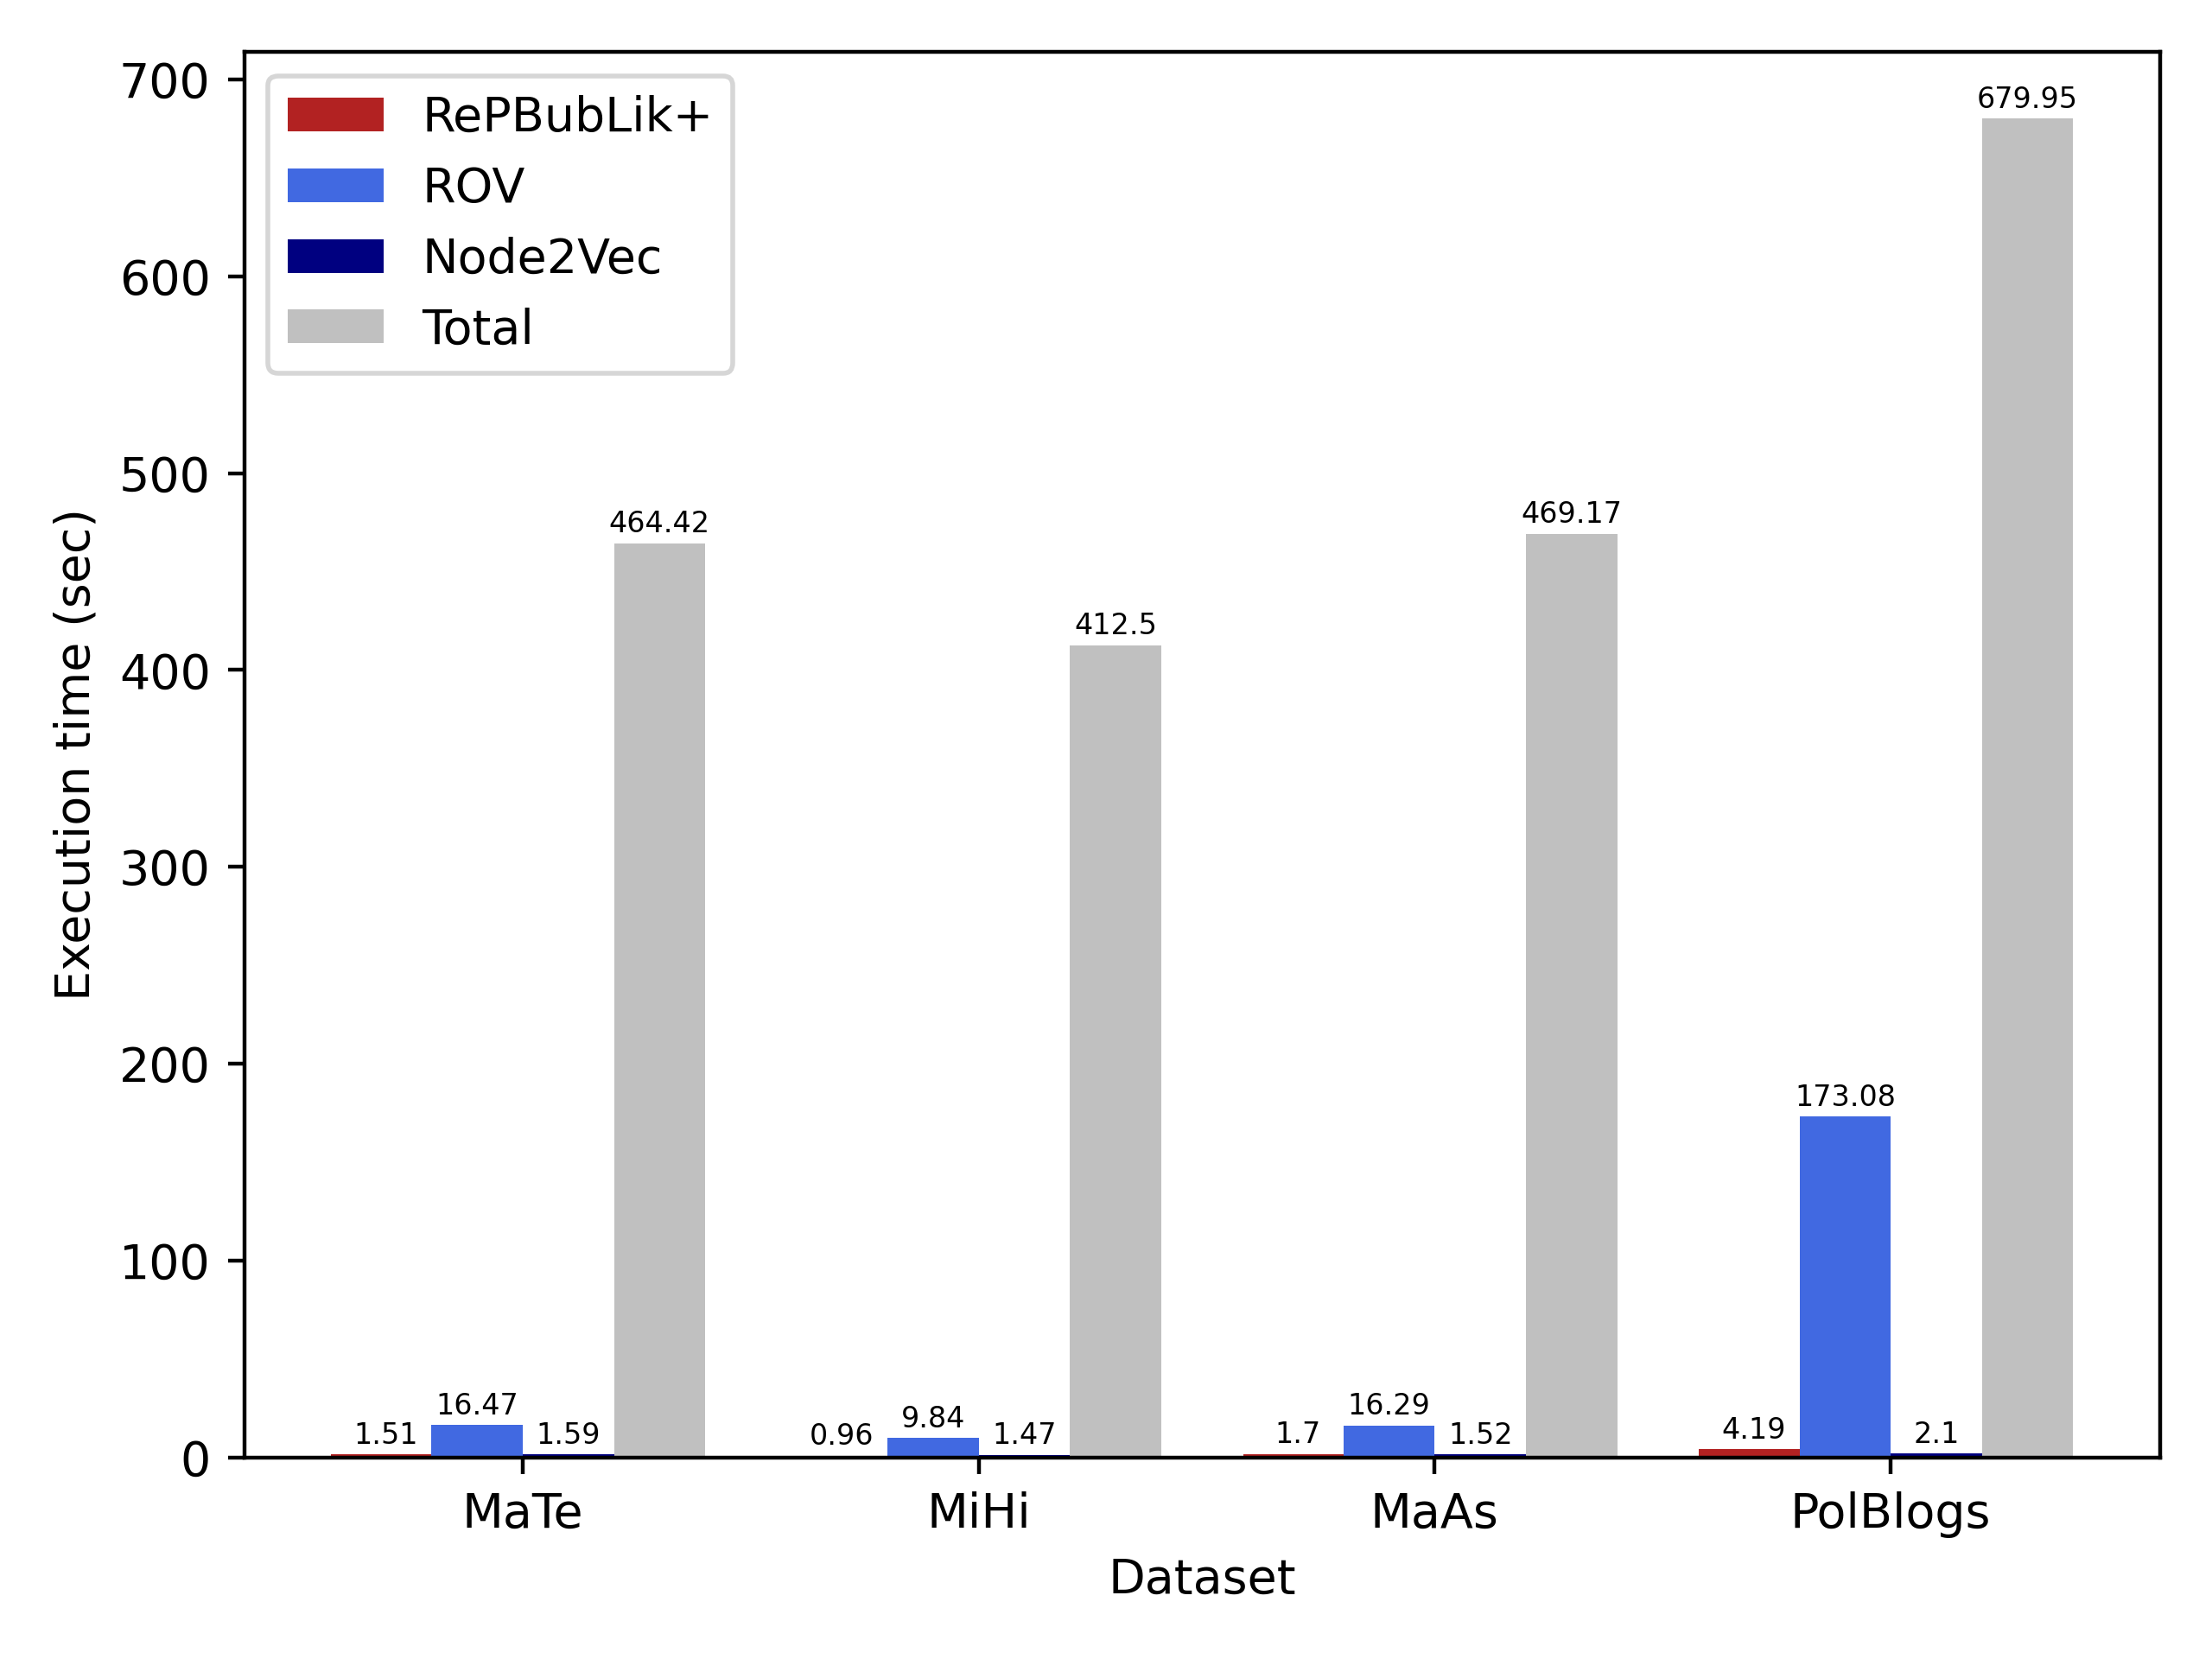
\includegraphics[width=\columnwidth]{5/ex_time_5.png}
    \caption{Parametro $t=5$}\label{fig:mate_e_5}
\end{subfigure}
\begin{subfigure}[h]{0.55\columnwidth}
    \centering
    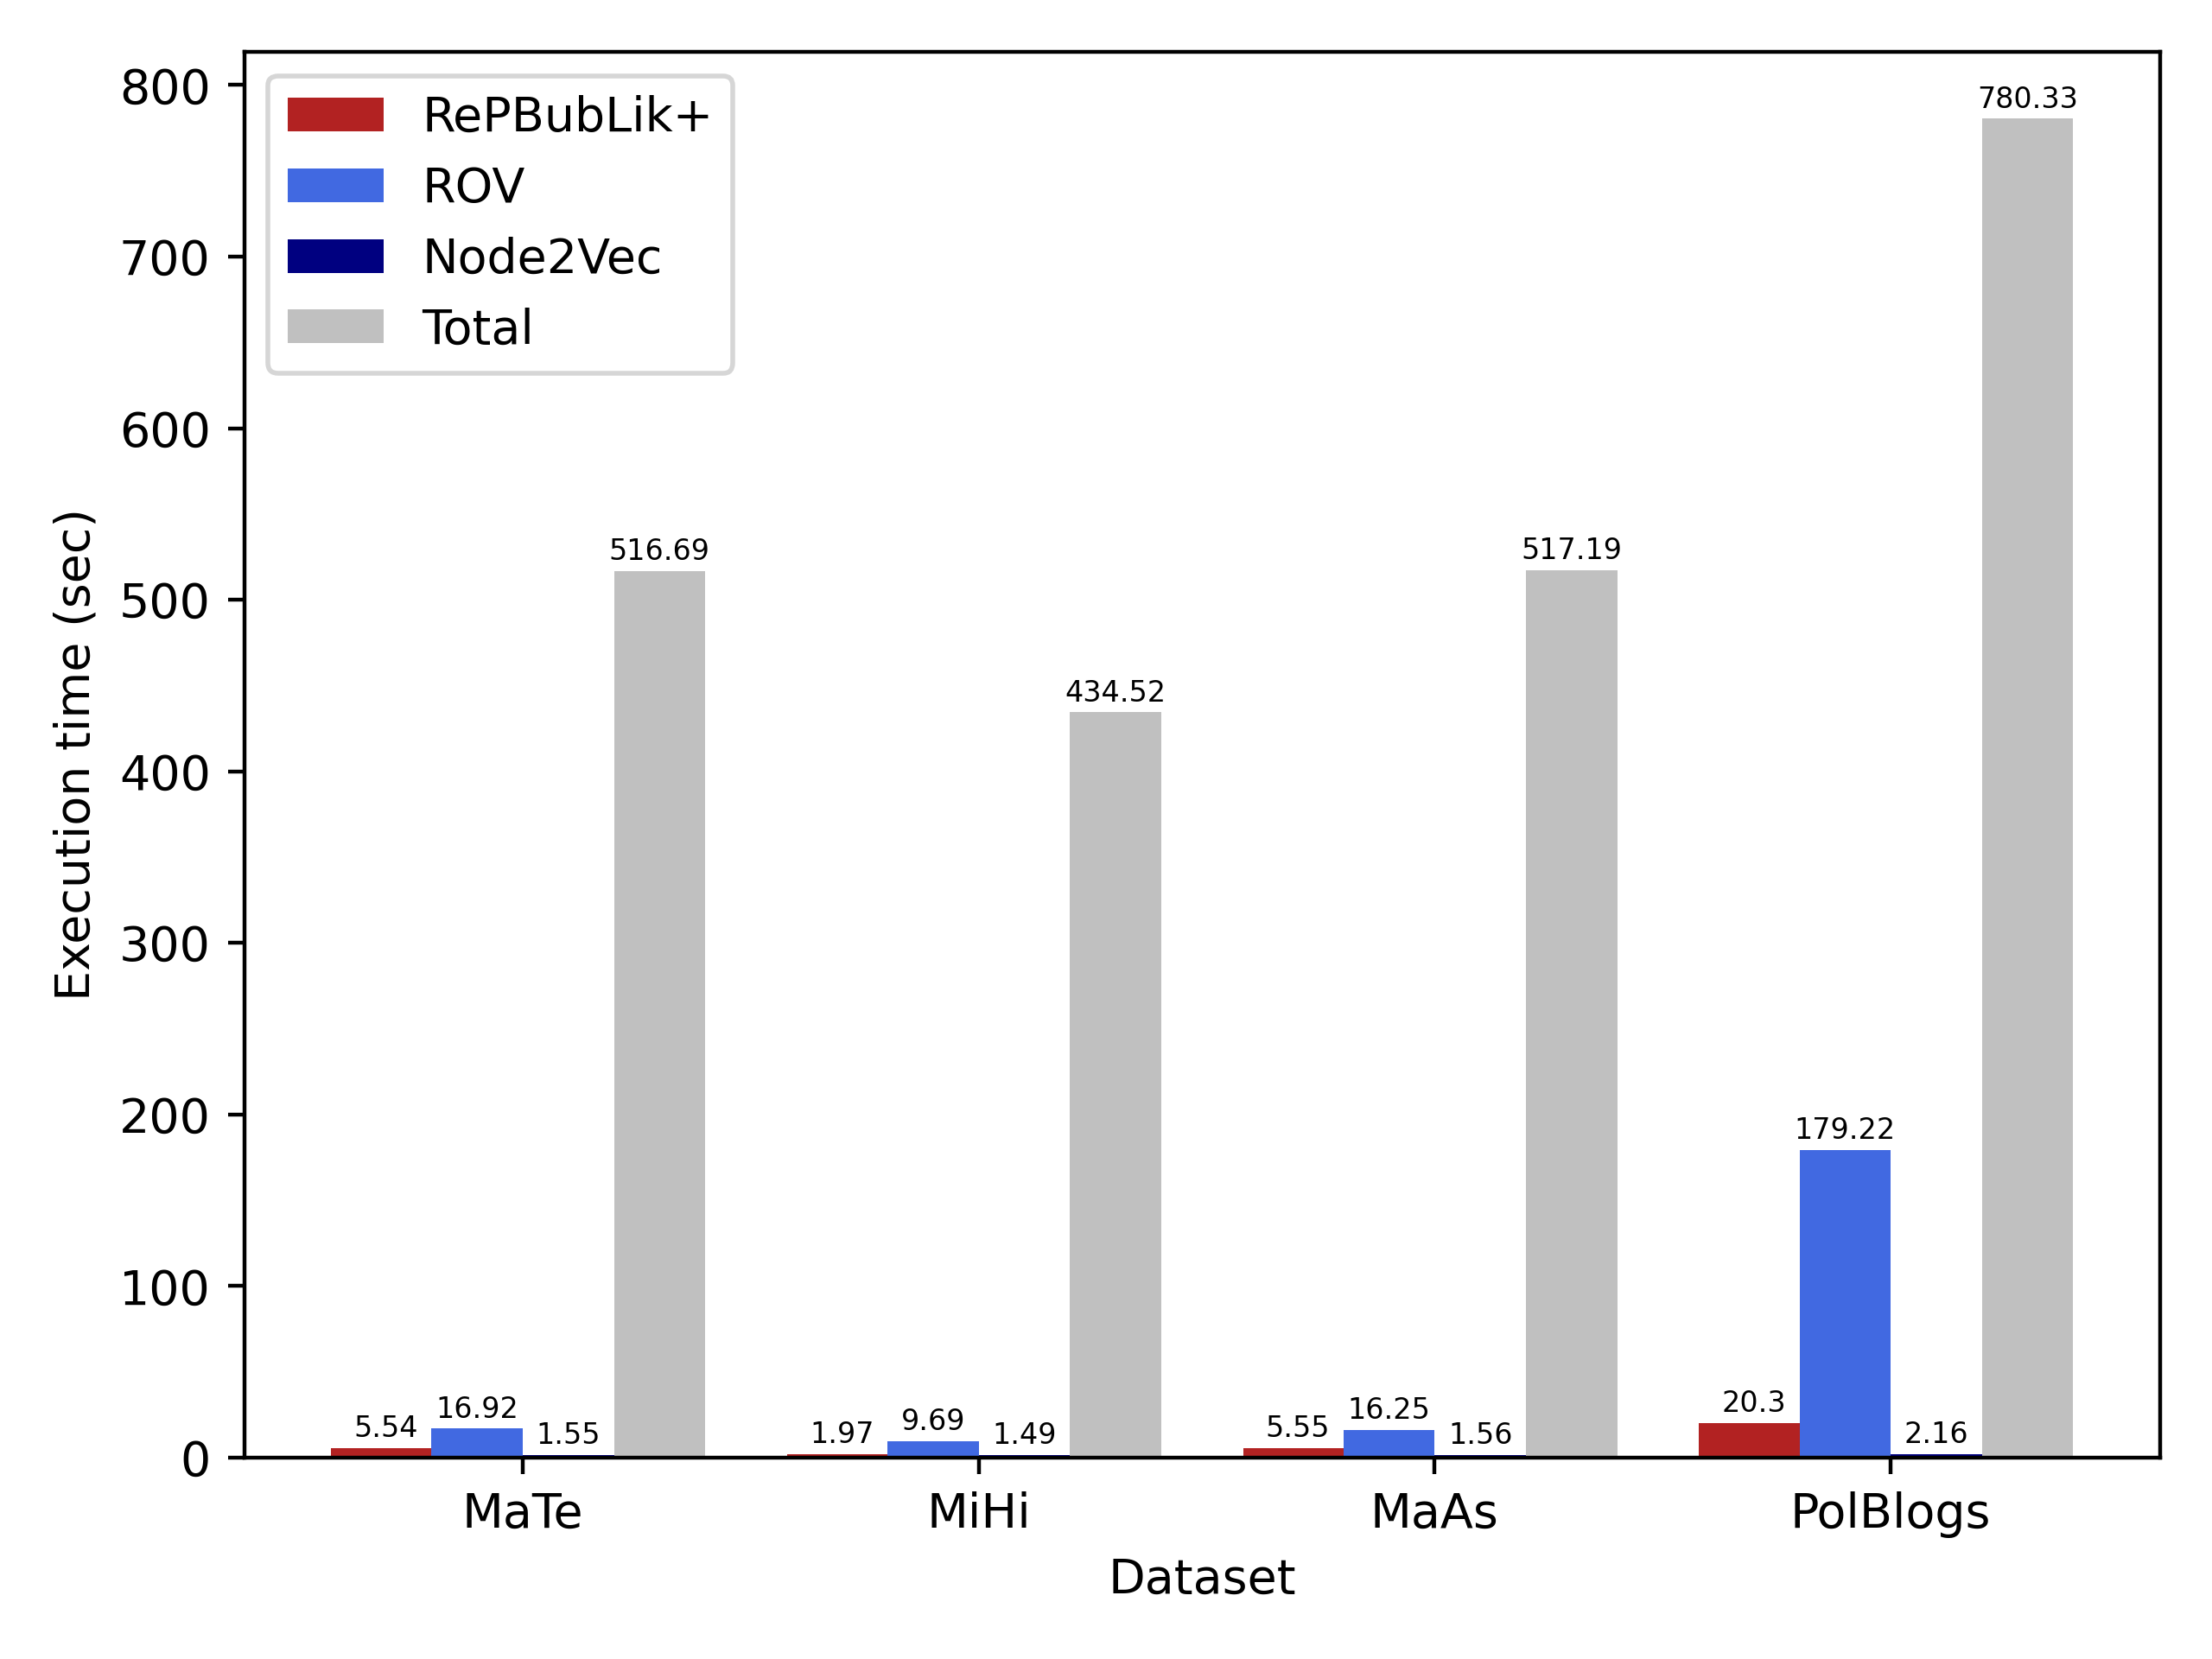
\includegraphics[width=\columnwidth]{10/ex_time_10.png}
    \caption{Parametro $t=10$}\label{fig:mihi_e_10}
\end{subfigure}
   
\end{figure}
\begin{figure}
\ContinuedFloat
\centering
\begin{subfigure}[h]{0.55\columnwidth}
    \centering
    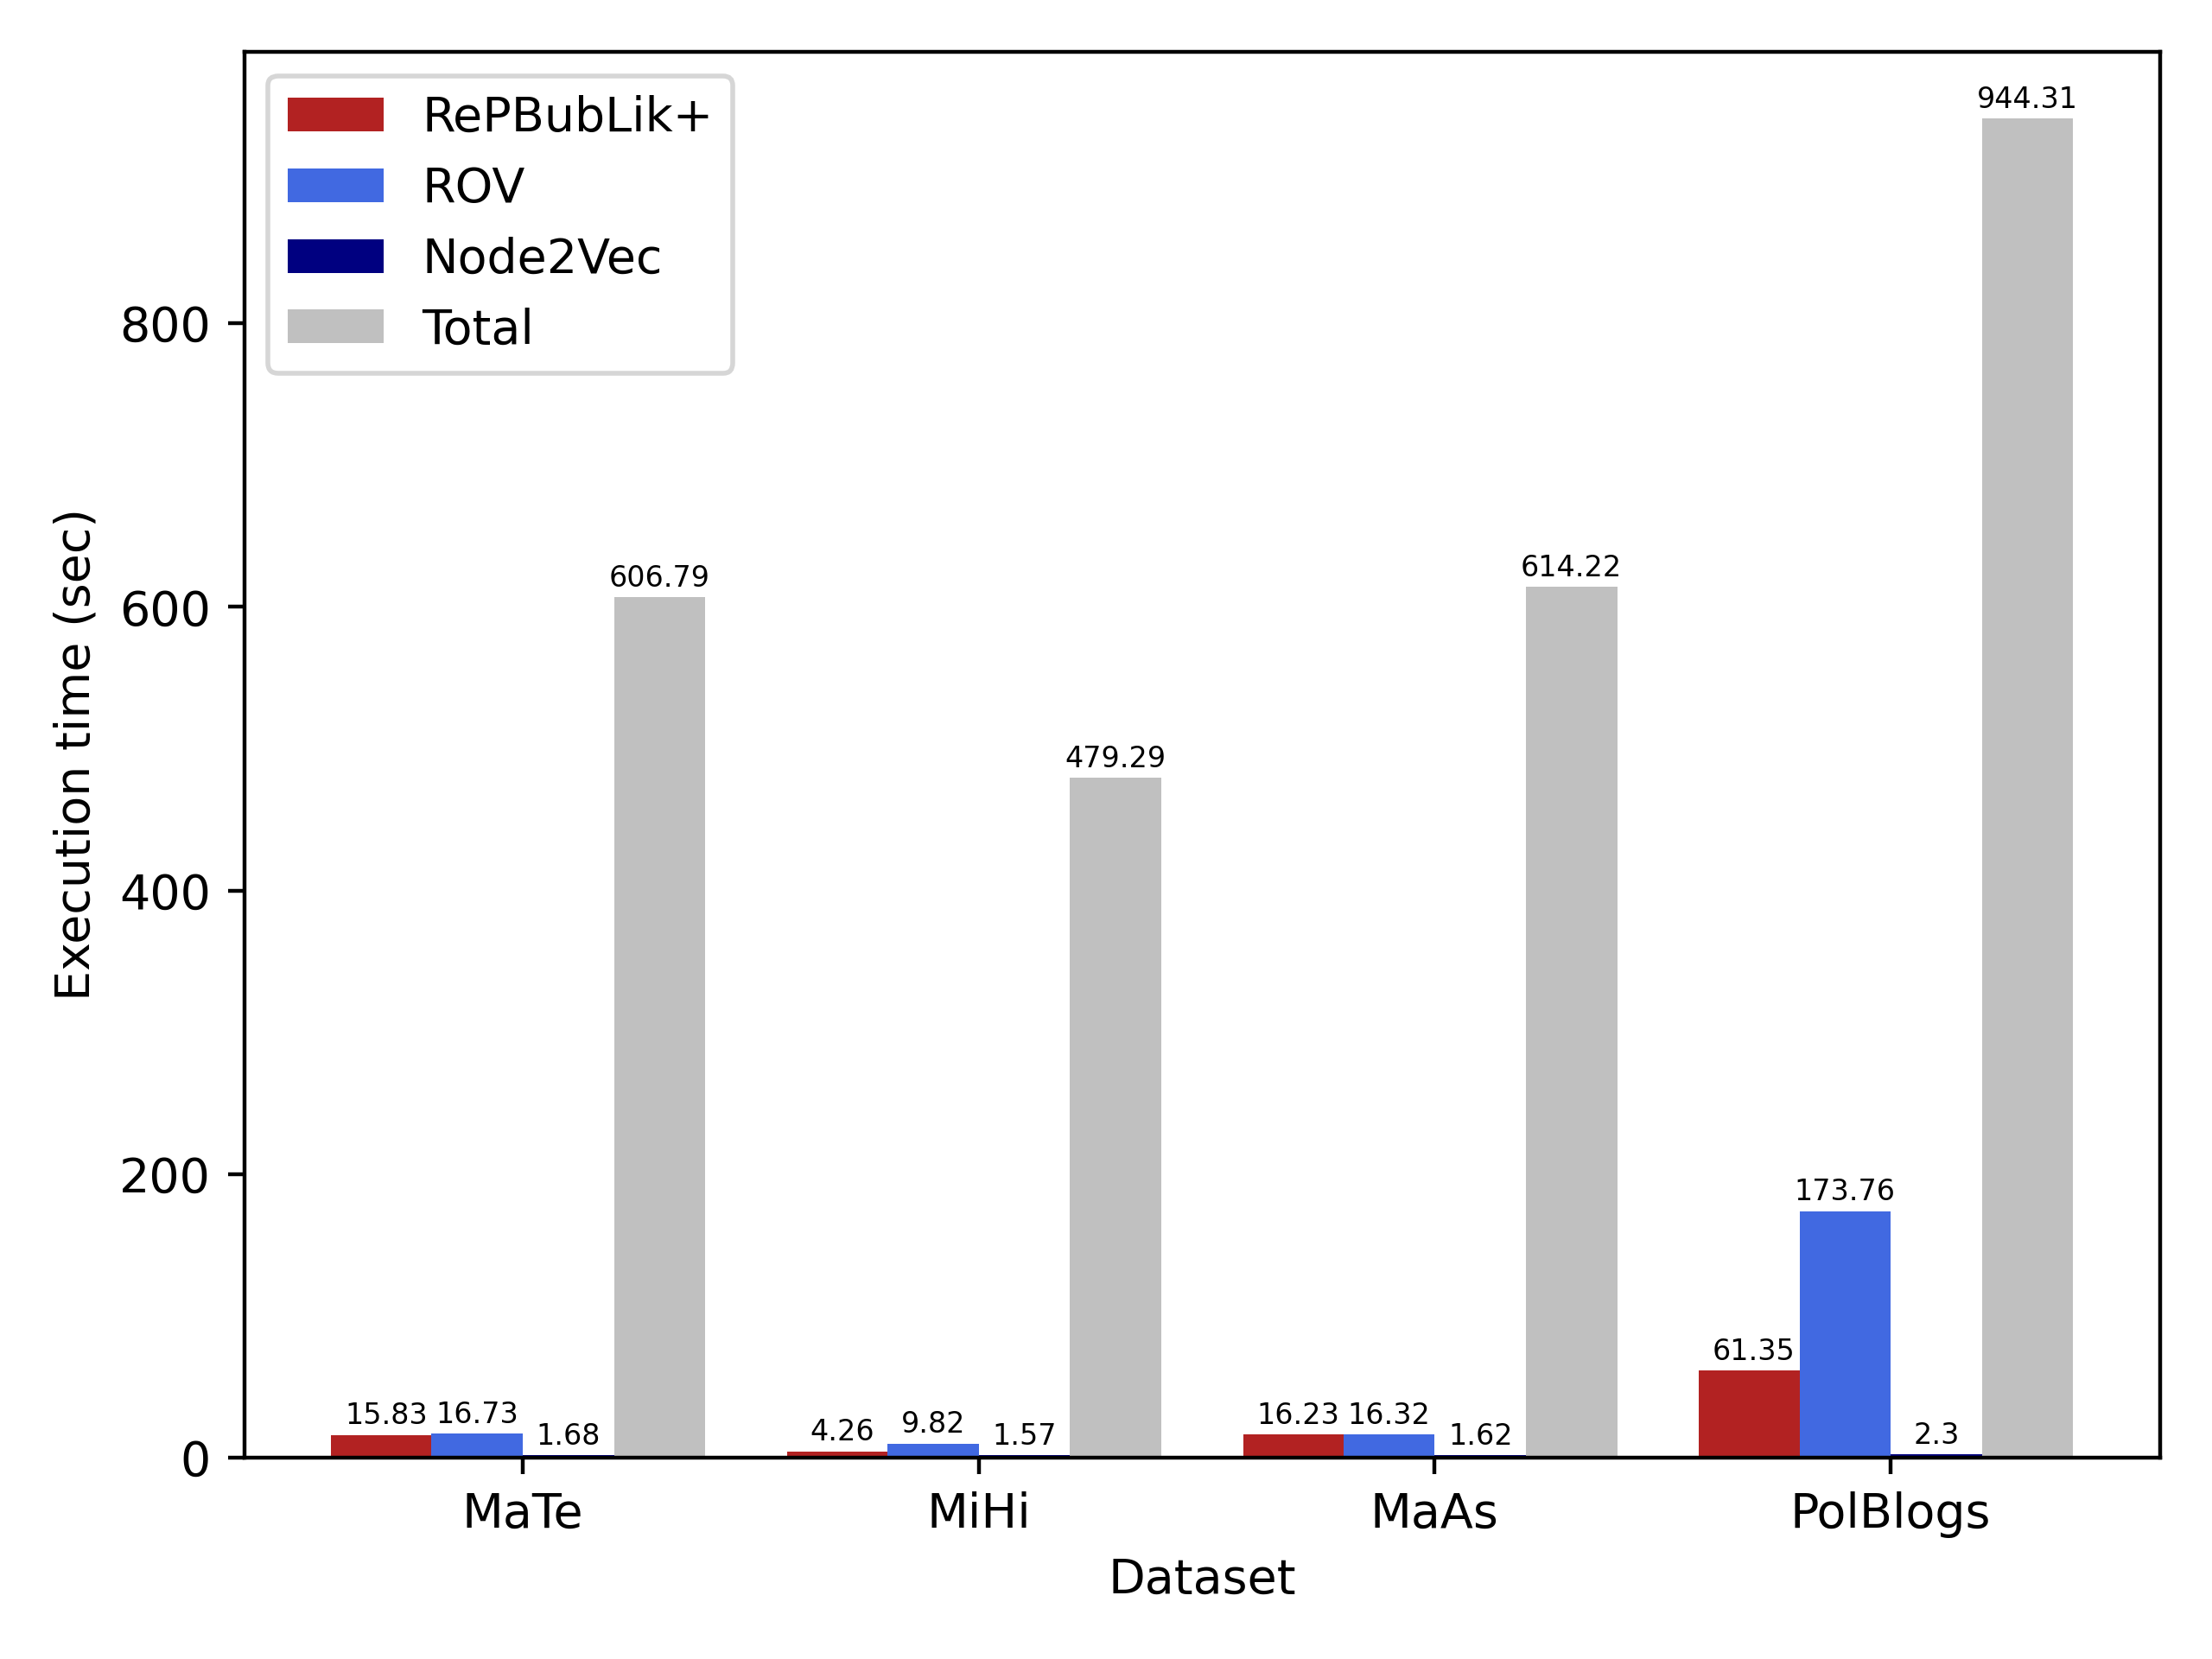
\includegraphics[width=\columnwidth]{15/ex_time_15.png}
    \caption{Parametro $t=15$}\label{fig:maas_e_15}
\end{subfigure}
\caption{Grafici dei tempi d'esecuzione}
\end{figure}
\newpage
Analizzando i grafici dei tempi di esecuzione, si possono trarre le seguenti conclusioni:
\begin{enumerate}
    \item Il tempo impiegato da ciascuna procedura aumenta in relazione alle dimensioni del grafo su cui è applicata.
    \item Node2Vec risulta essere il migliore in termini di tempo d'esecuzione, per ogni grafo e per ogni valore di $t$.
    \item Per ciascun grafo, l'esecuzione di ROV impiega all'incirca lo stesso tempo, indipendentemente dal valore di $t$. 
            Questo è dato dal fatto che ROV utilizza delle metriche differenti dagli altri algoritmi proposti.
    \item RePBubLik+ ha tempistiche intermedie tra quelle di ROV e Node2Vec.
\end{enumerate}
\subsection{Guadagno $\Delta(G,\Sigma)$}
La seconda metrica che viene anlizzata è il il guadagno $\Delta(G,\Sigma)$ (\ref{REP:gain}) in relazione al numero 
degli archi aggiunti al grafo $G$. Lo studio di questa misura è interessante, in quanto permette di valutare il cambiamento medio del Bubble Radius dei vertici parochial $P(G)$.
\\
Nella pagina successiva, i guadagni per ciascun grafo e per ciascun valore di $t$.
\begin{figure}[!h]
    \centering
\begin{subfigure}[h]{0.4\textwidth}
    \centering
    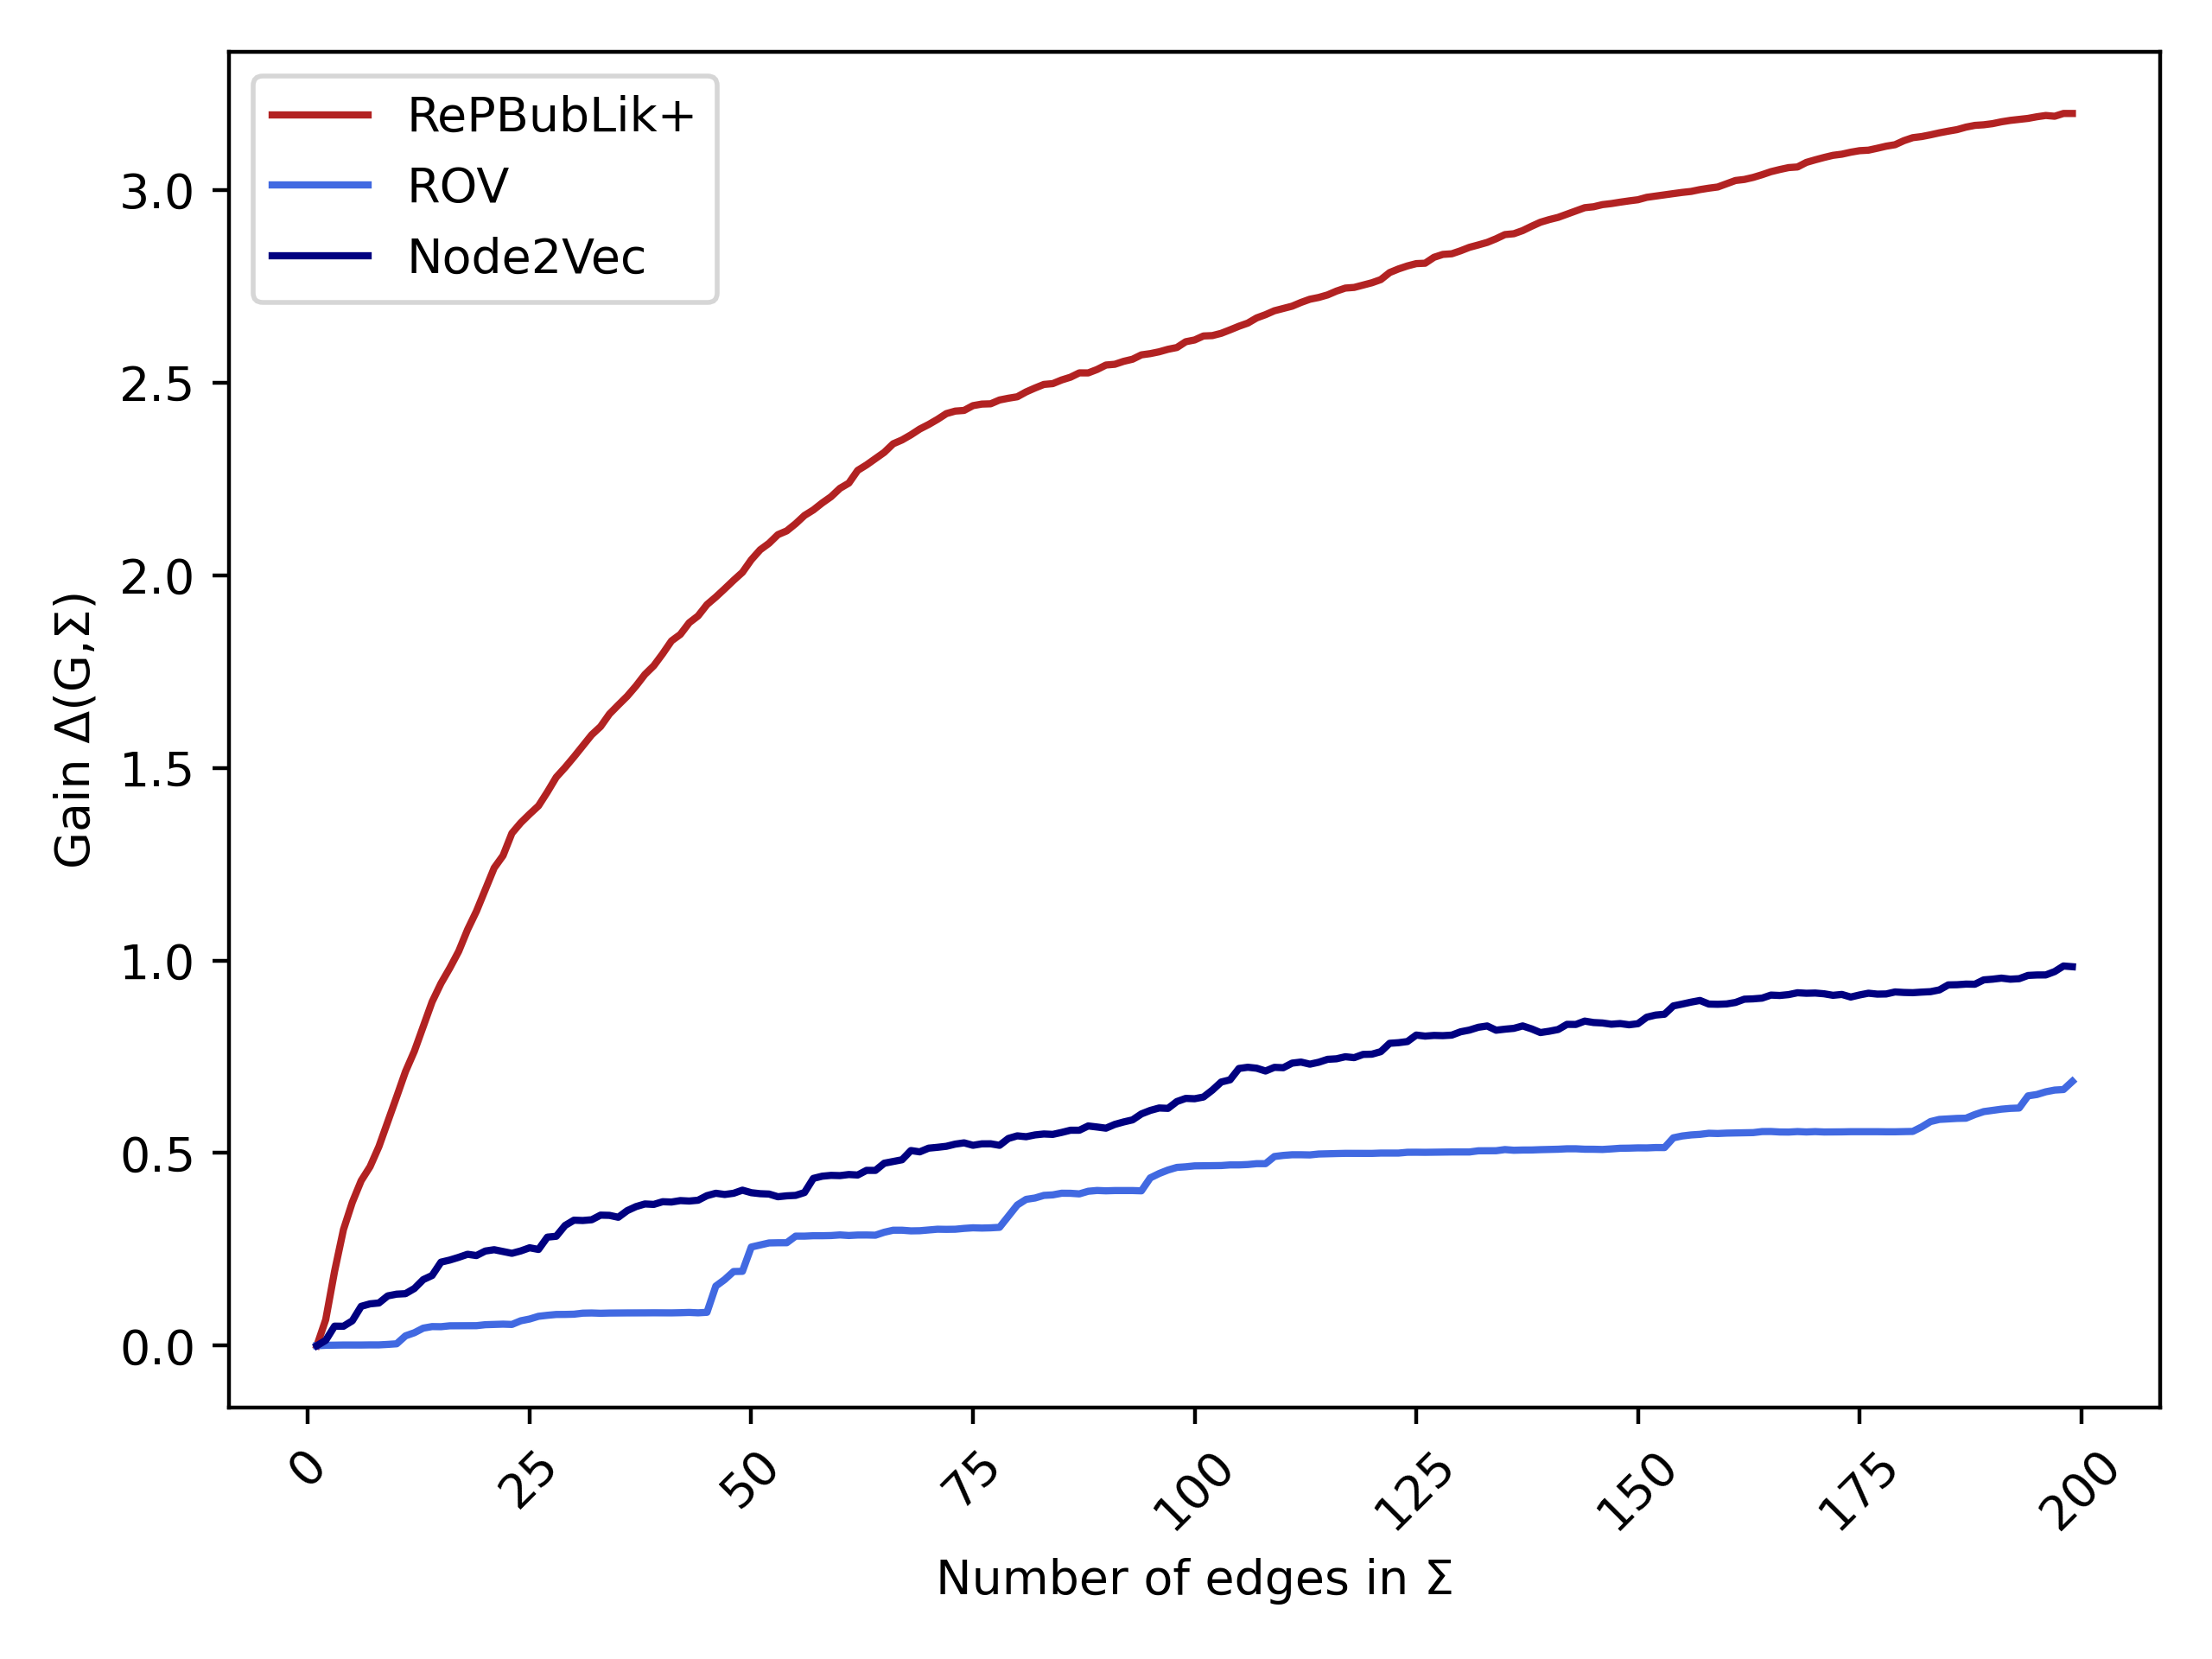
\includegraphics[width=\columnwidth]{5/math_tech_gain_5.png}
    \caption{\emph{MaTe} plot}\label{fig:mate_g_5}
\end{subfigure}
\hspace{0.1\columnwidth}
\begin{subfigure}[h]{0.4\textwidth}
    \centering
    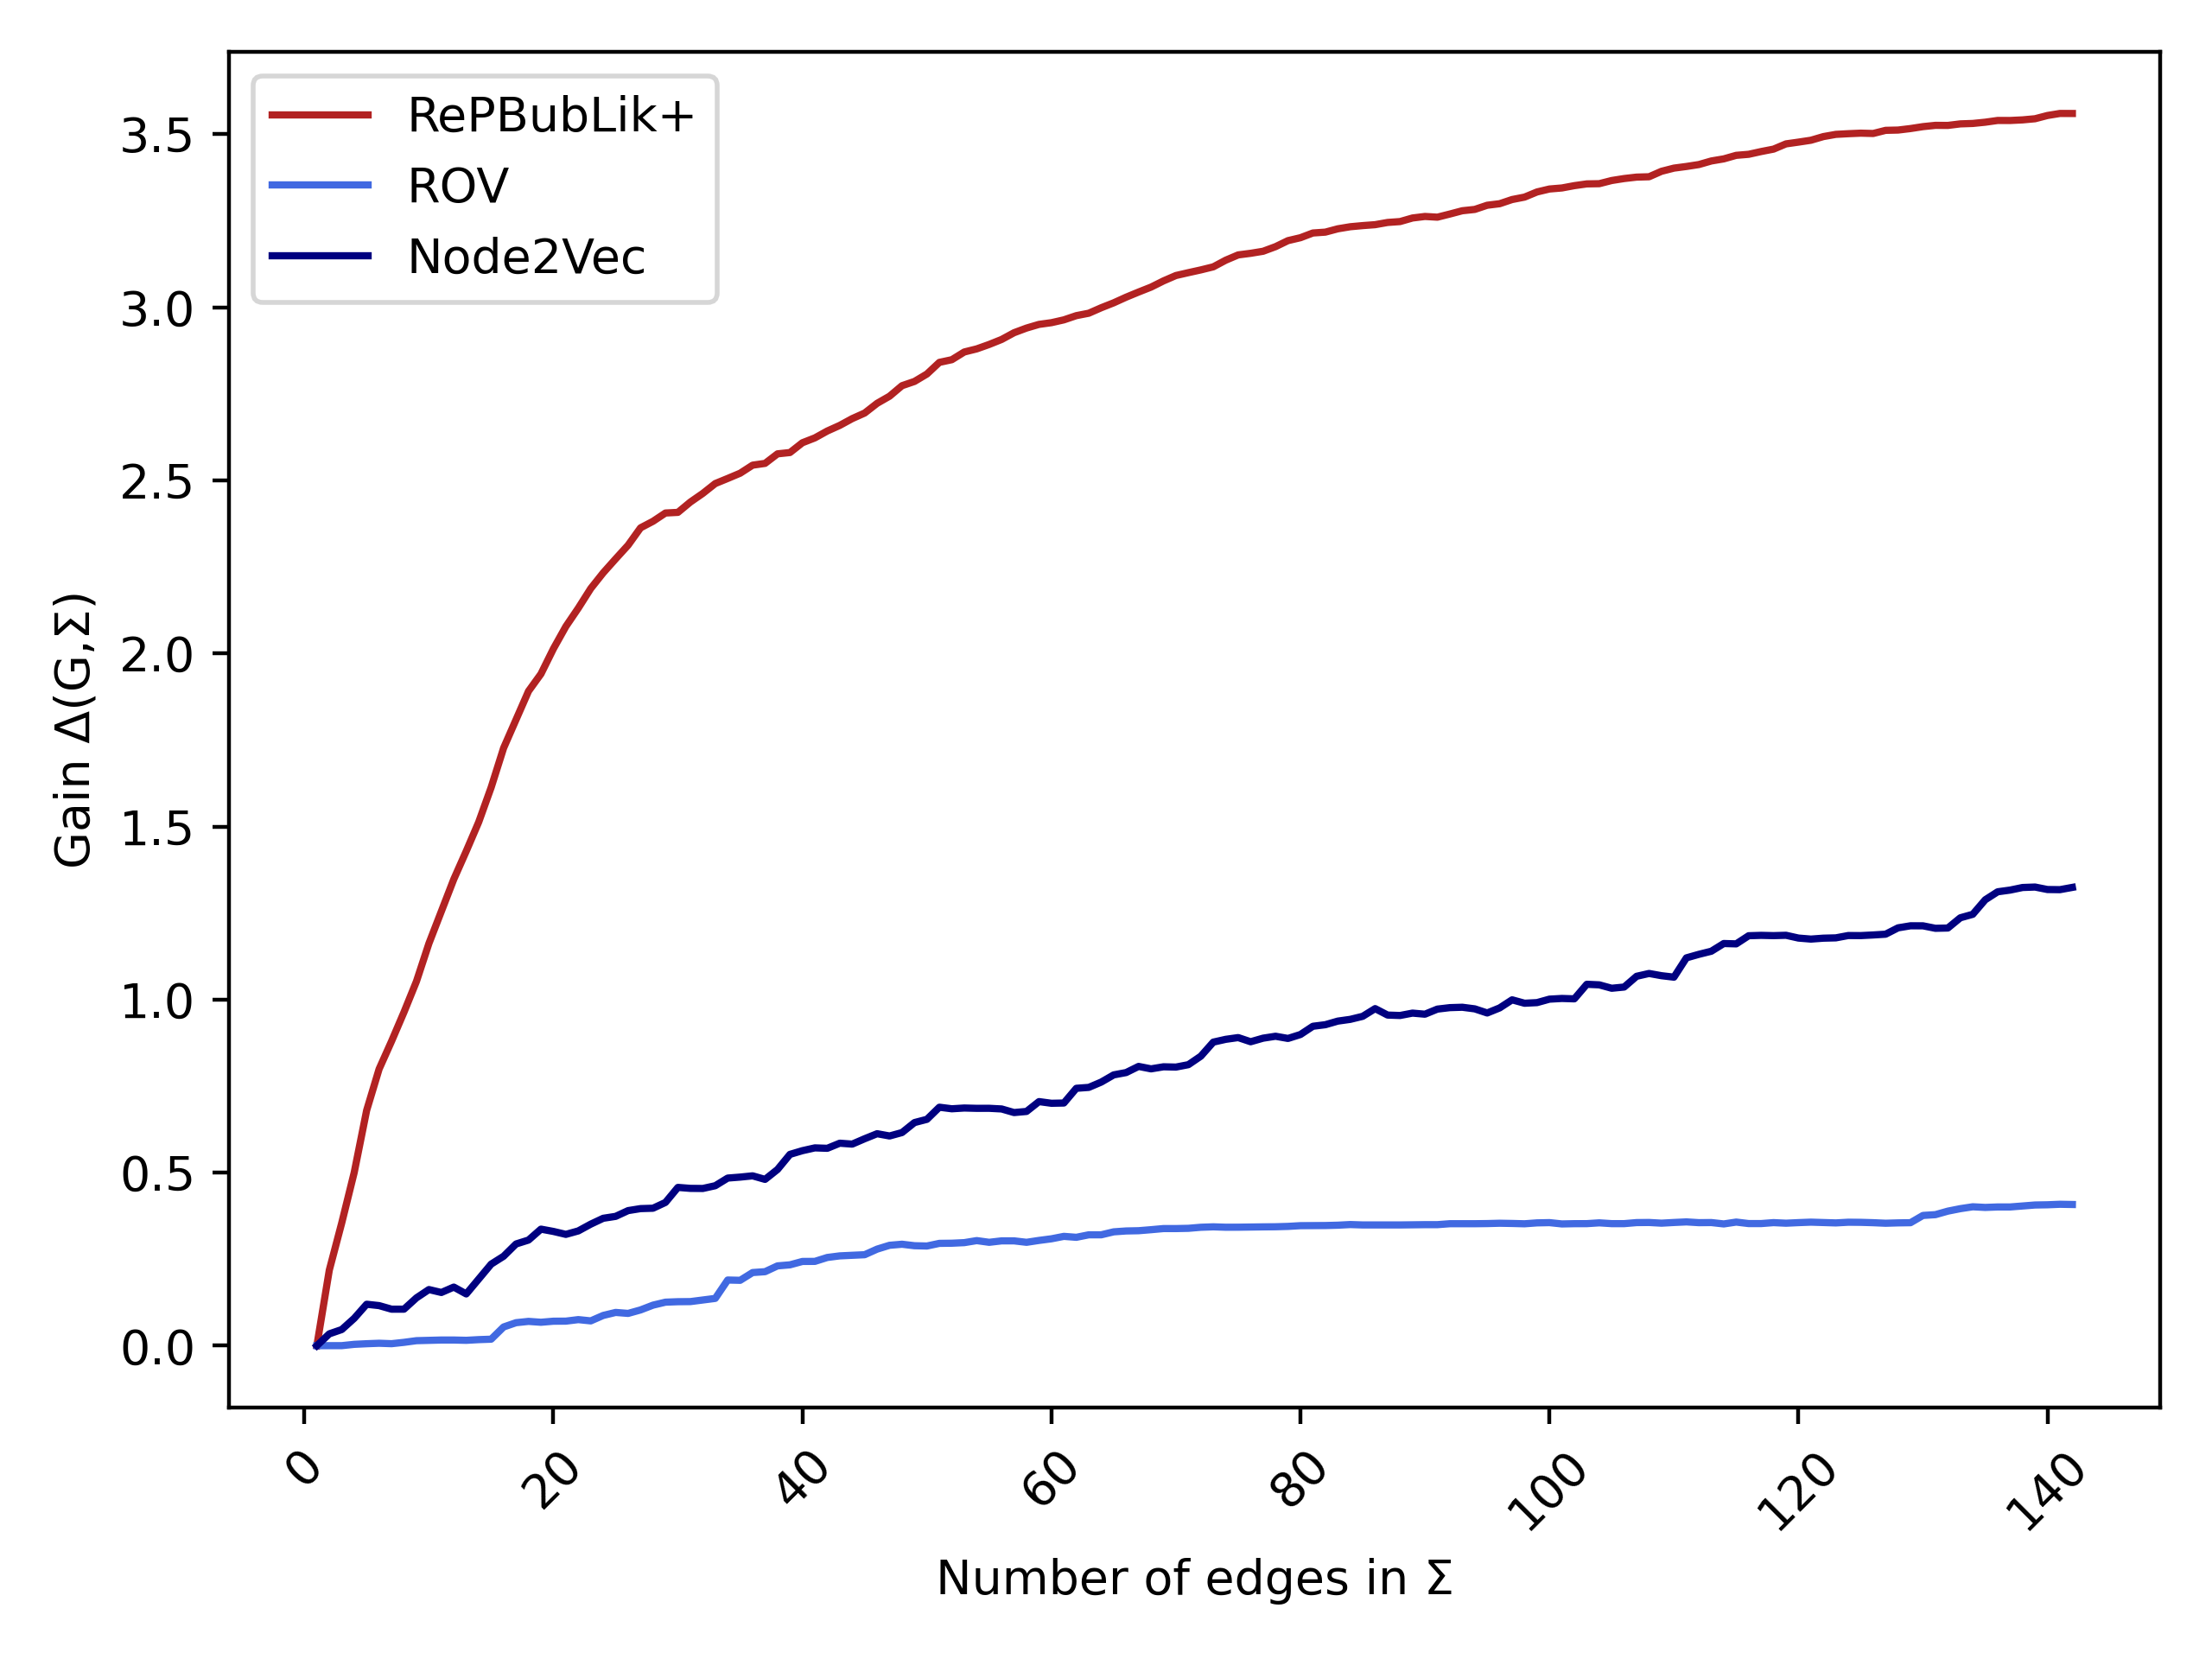
\includegraphics[width=\columnwidth]{5/tech_mil_gain_5.png}
    \caption{\emph{MiHi} plot}\label{fig:mihi_g_5}
\end{subfigure}
\end{figure}
\begin{figure}
    \ContinuedFloat
    \centering
\begin{subfigure}[h]{0.4\textwidth}
    \centering
    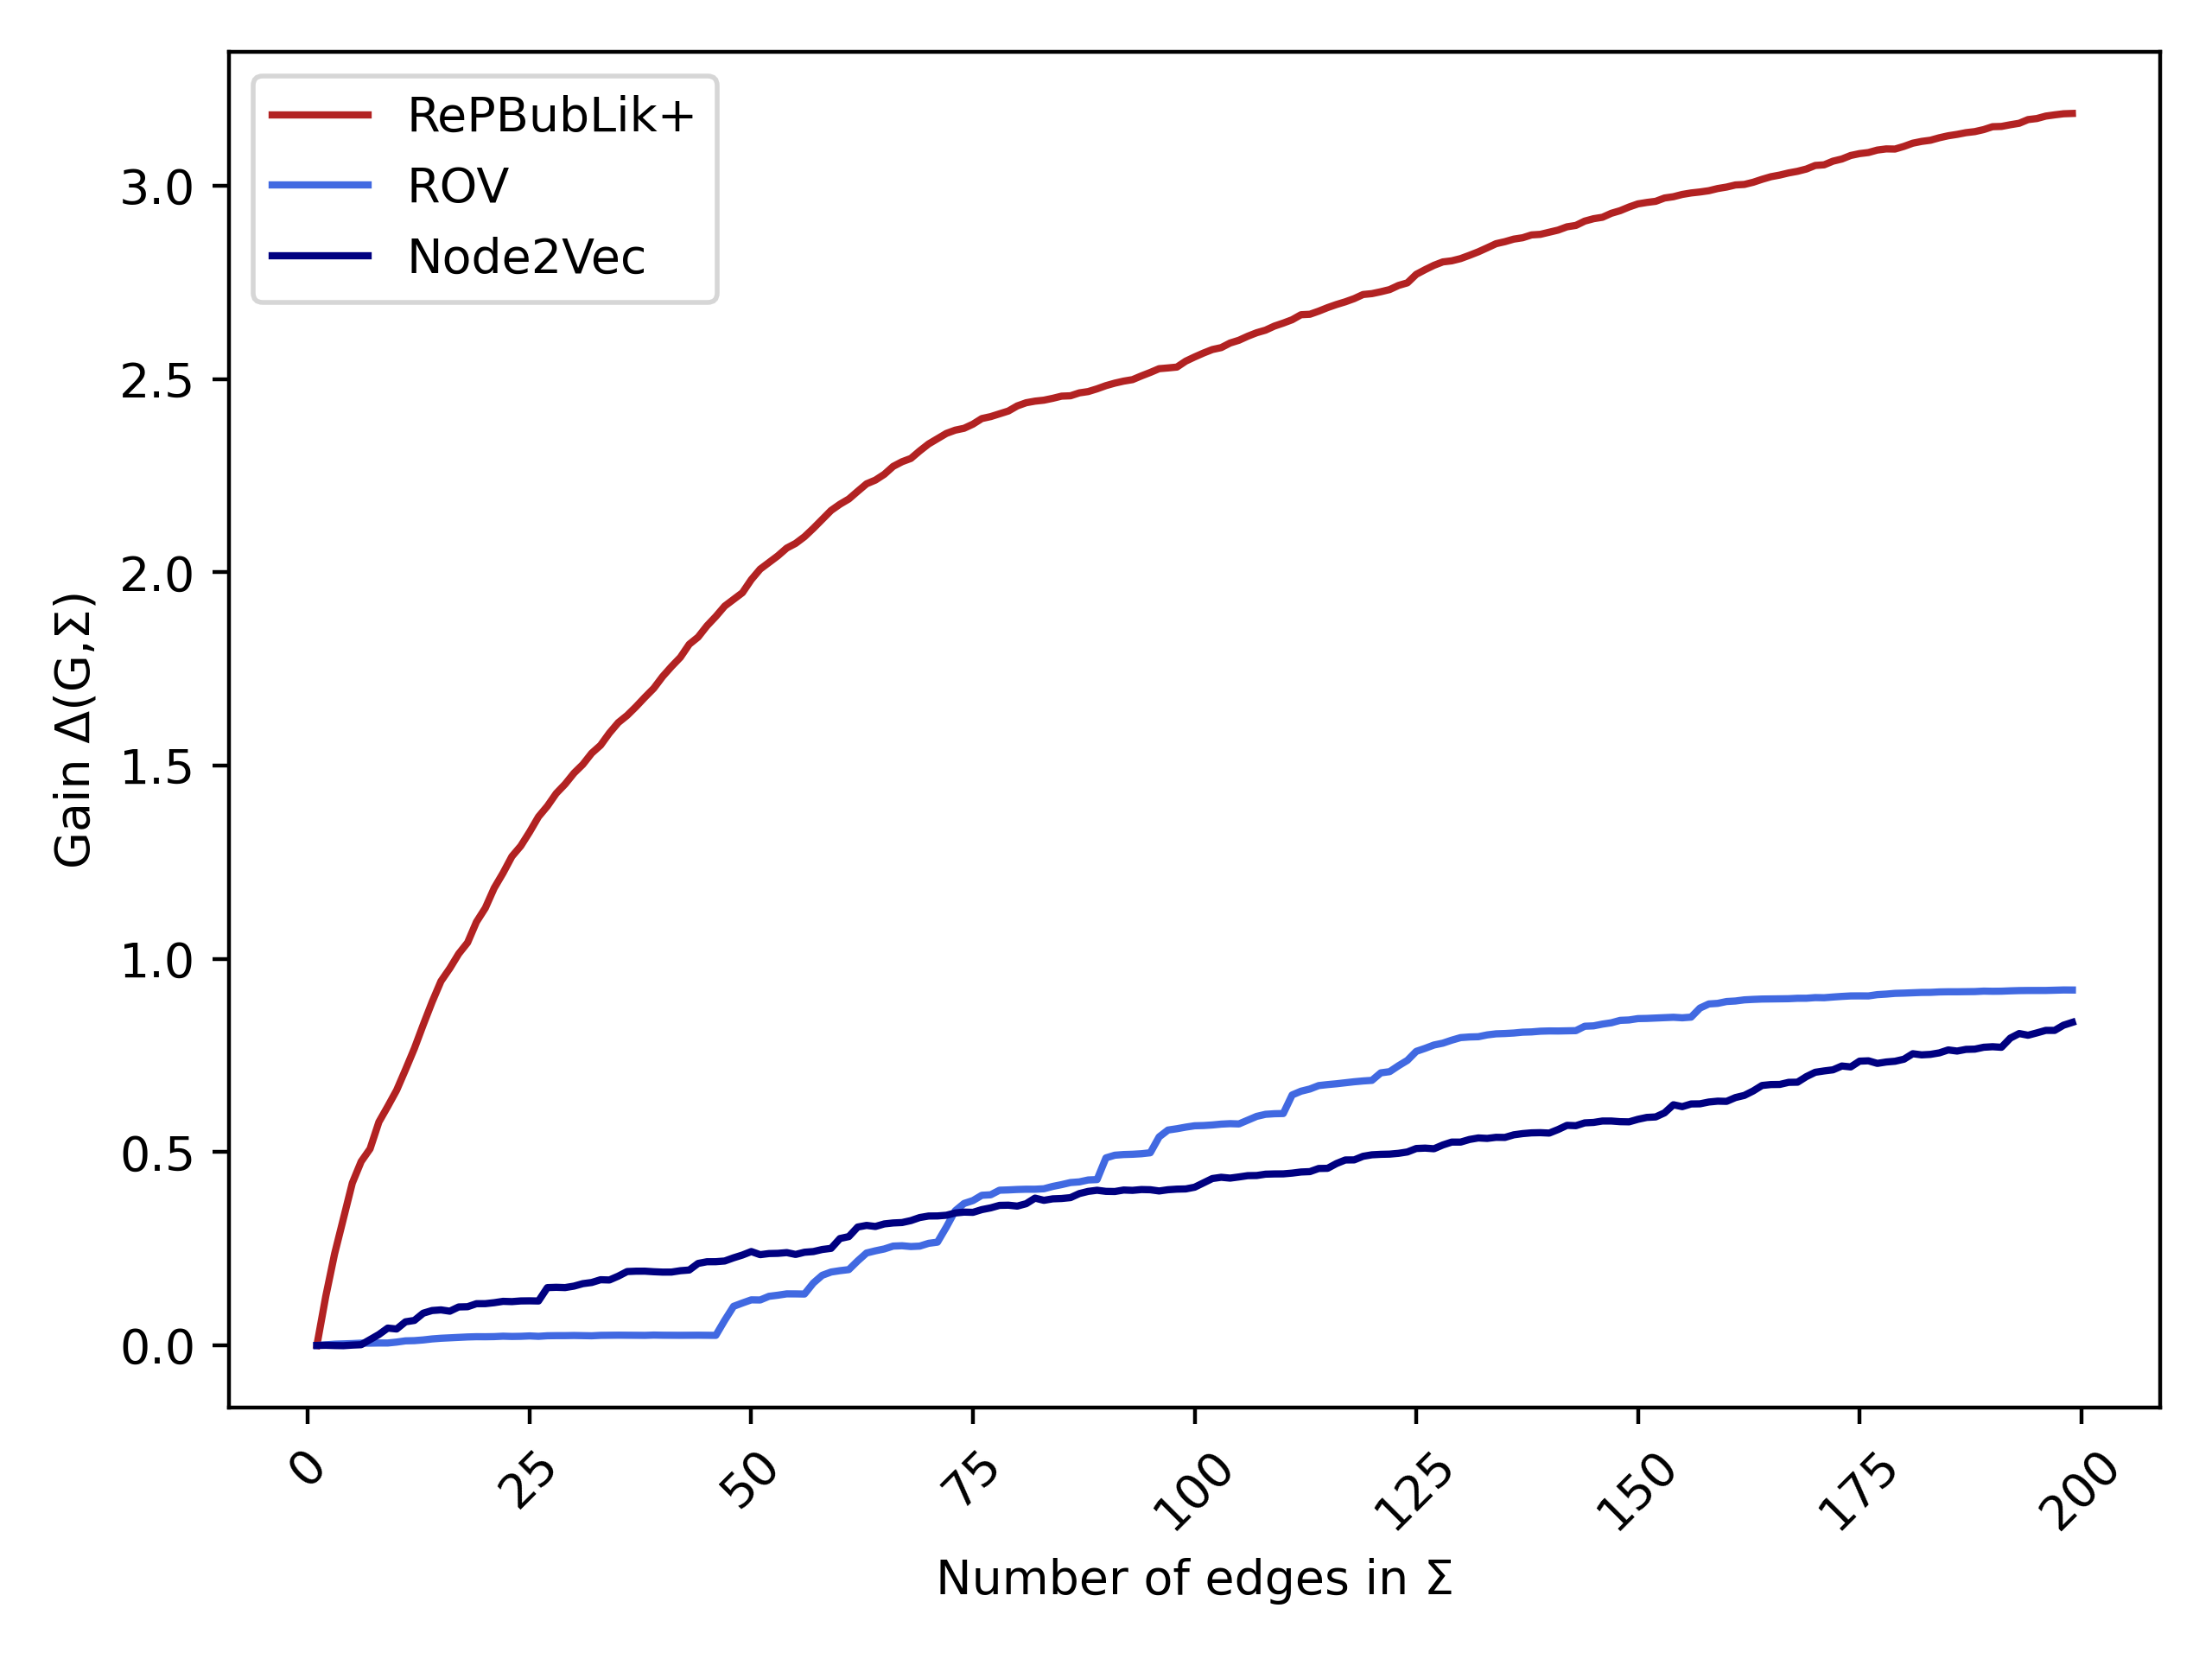
\includegraphics[width=\columnwidth]{5/math_ast_gain_5.png}
    \caption{\emph{MaA}s plot}\label{fig:maas_g_5}
\end{subfigure}
\hspace{0.1\columnwidth}
\begin{subfigure}[h]{0.4\textwidth}
    \centering
    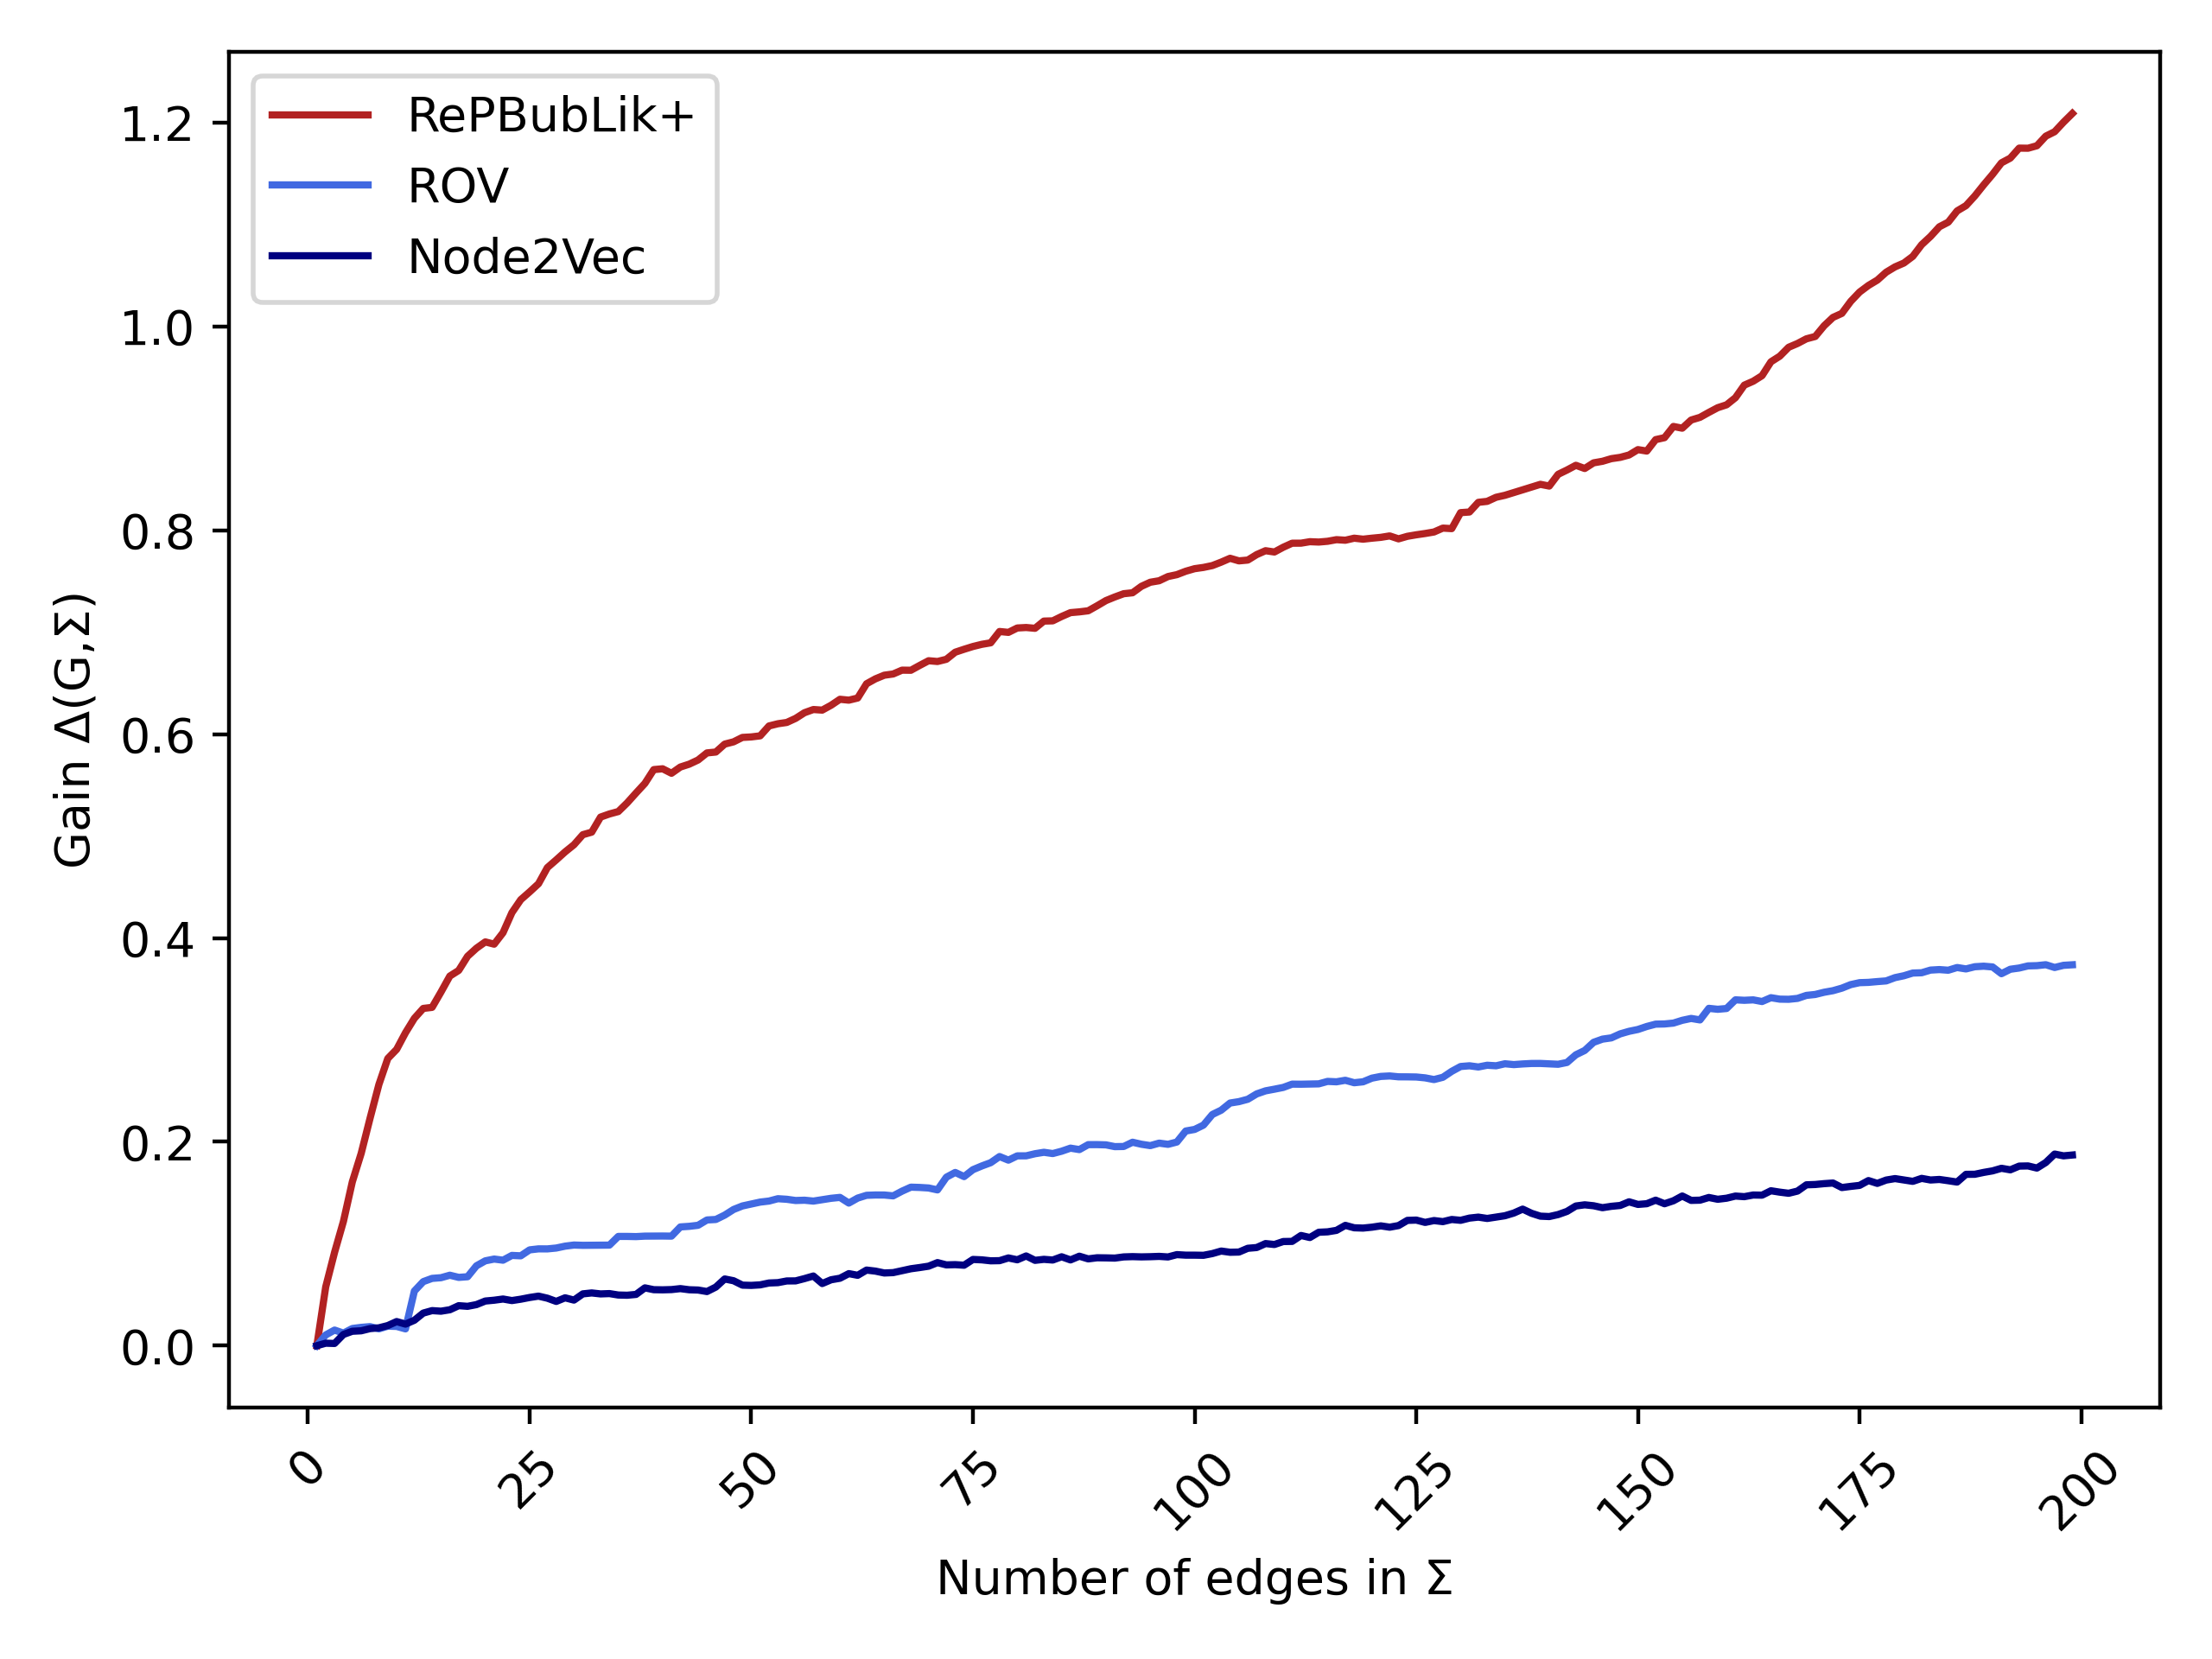
\includegraphics[width=\columnwidth]{5/polblogs_gain_5.png}
    \caption{\emph{PolBlogs} plot}\label{fig:polblogs_g_5}
\end{subfigure}
\caption{Grafici $\Delta(G,\Sigma)$ per $t=5$}
\end{figure}
\begin{figure}[!h]
    \centering
\begin{subfigure}[b]{0.4\textwidth}
    \centering
    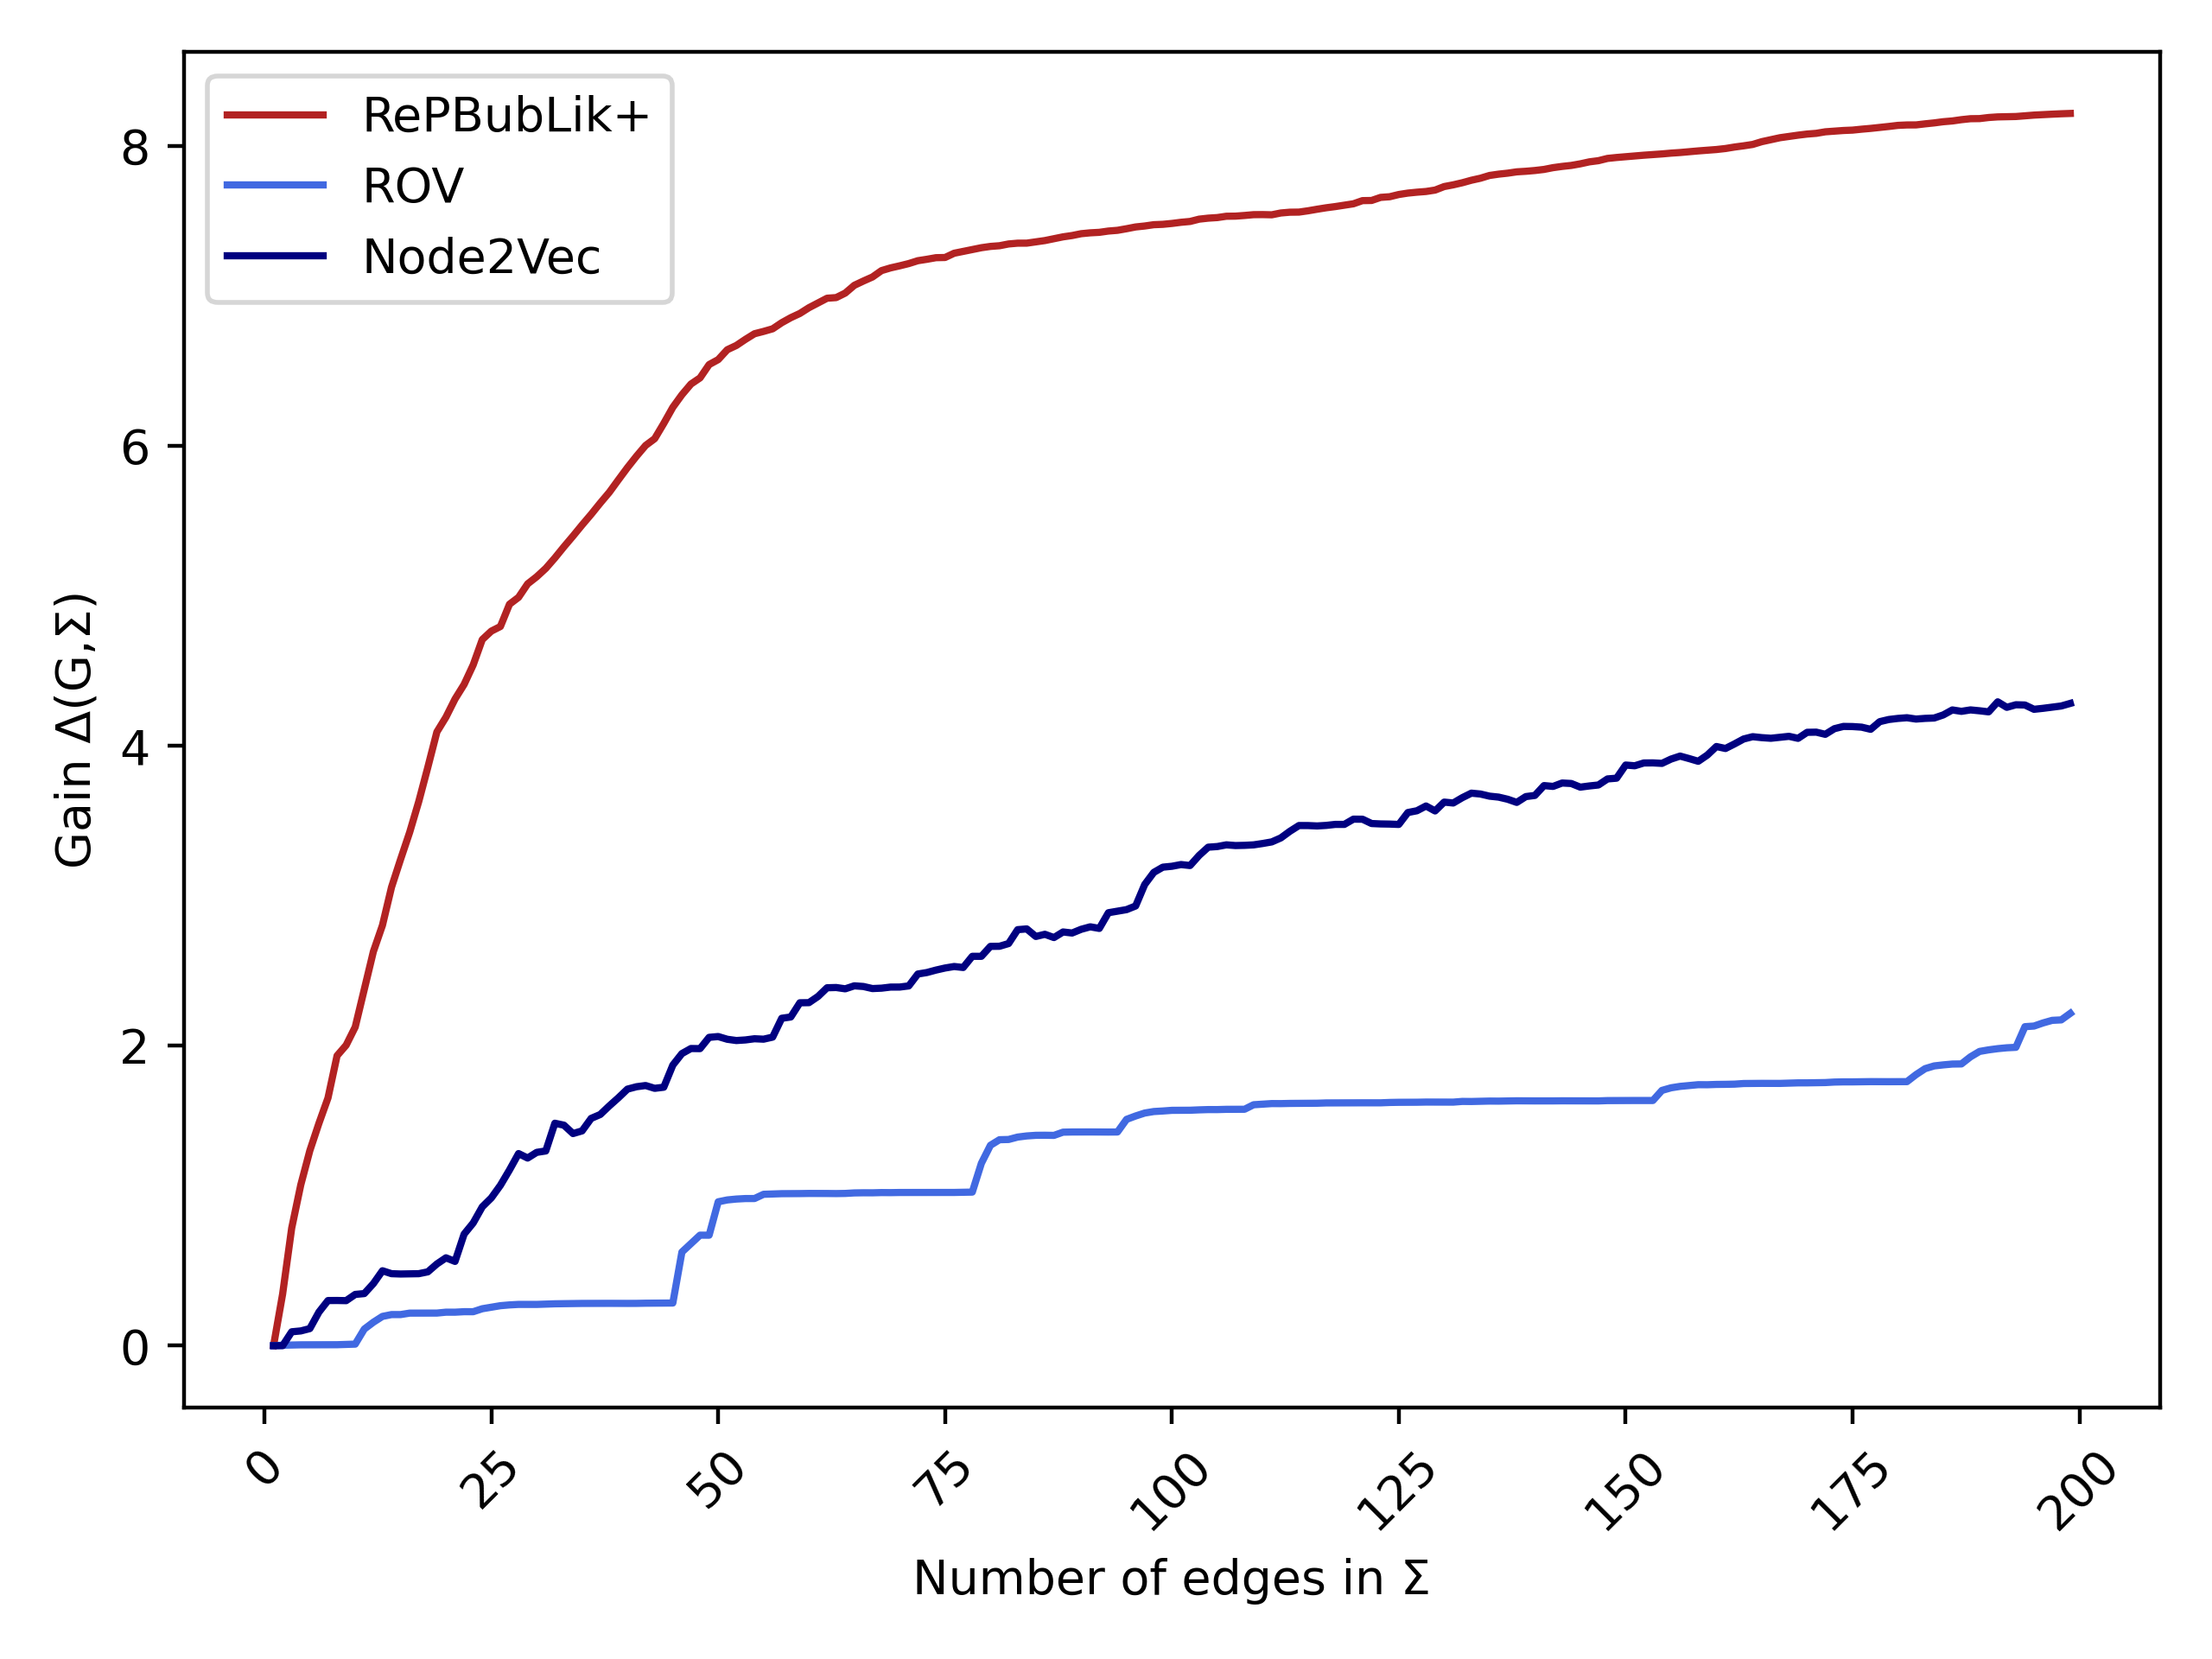
\includegraphics[width=\columnwidth]{10/math_tech_gain_10.png}
    \caption{\emph{MaTe} plot}\label{fig:mate_g_10}
\end{subfigure}
\hspace{0.1\columnwidth}
\begin{subfigure}[b]{0.4\textwidth}
    \centering
    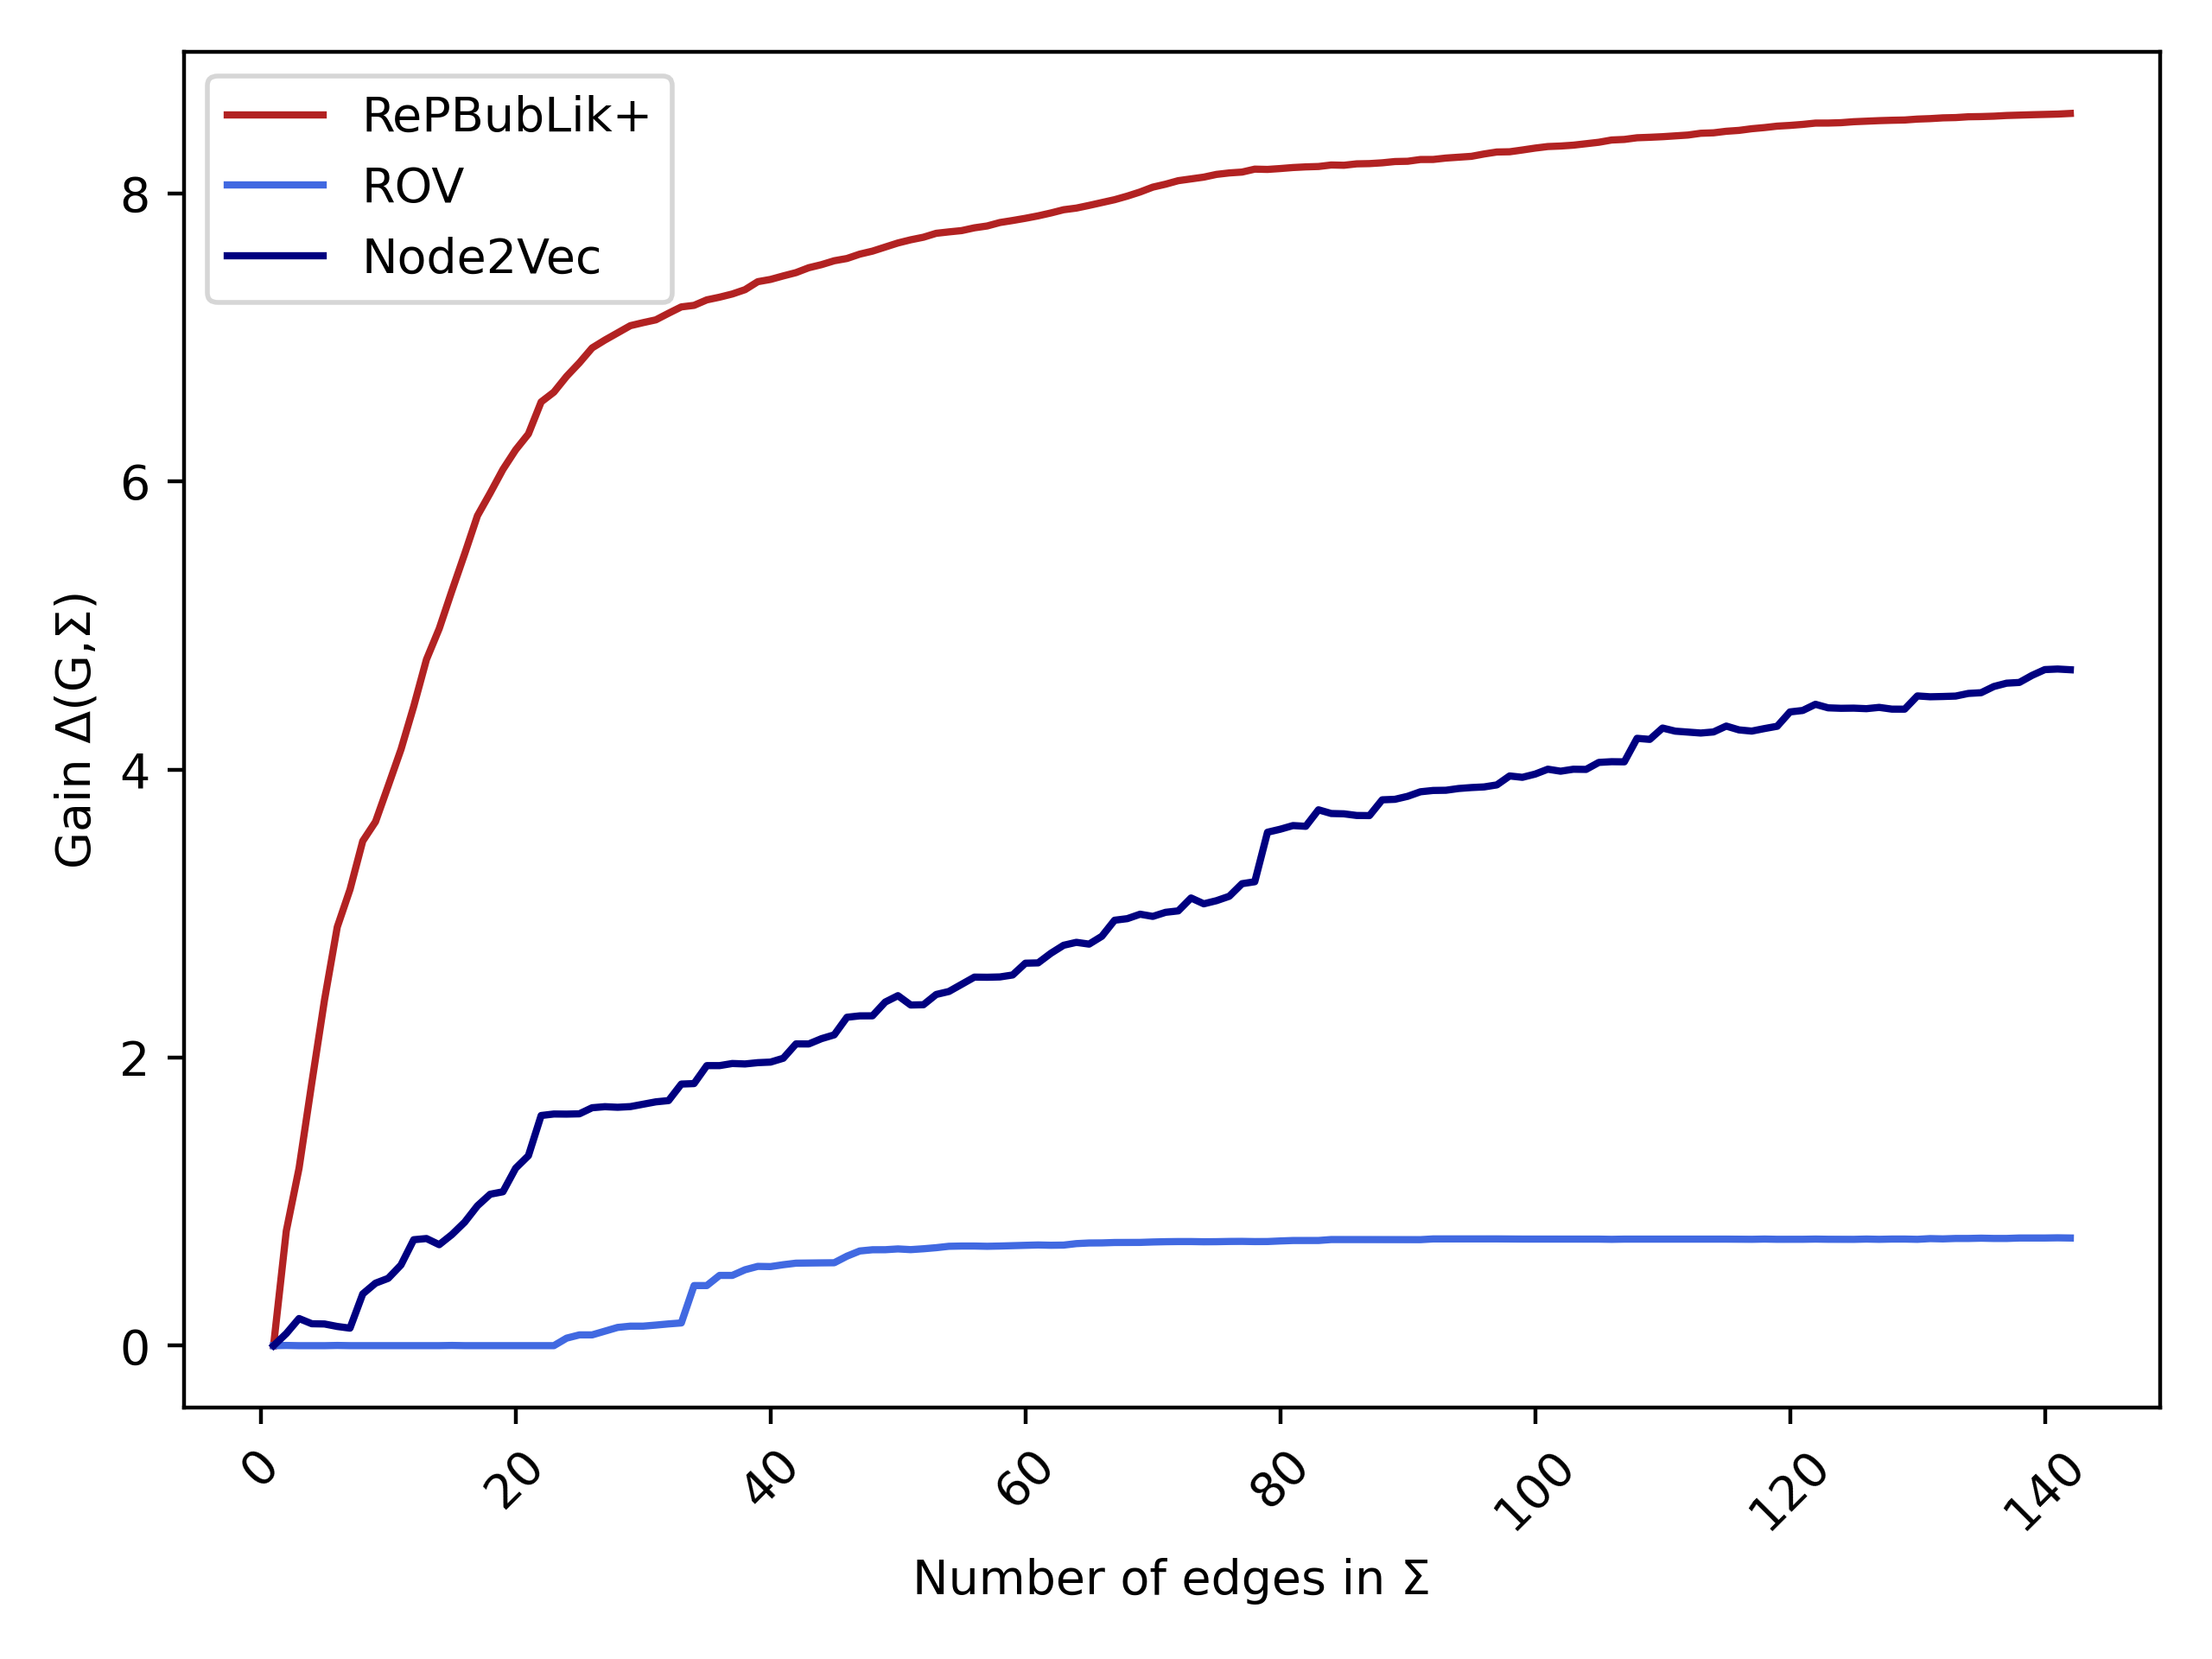
\includegraphics[width=\columnwidth]{10/tech_mil_gain_10.png}
    \caption{\emph{MiHi} plot}\label{fig:mihi_g_10}
\end{subfigure}

\begin{subfigure}[b]{0.4\textwidth}
    \centering
    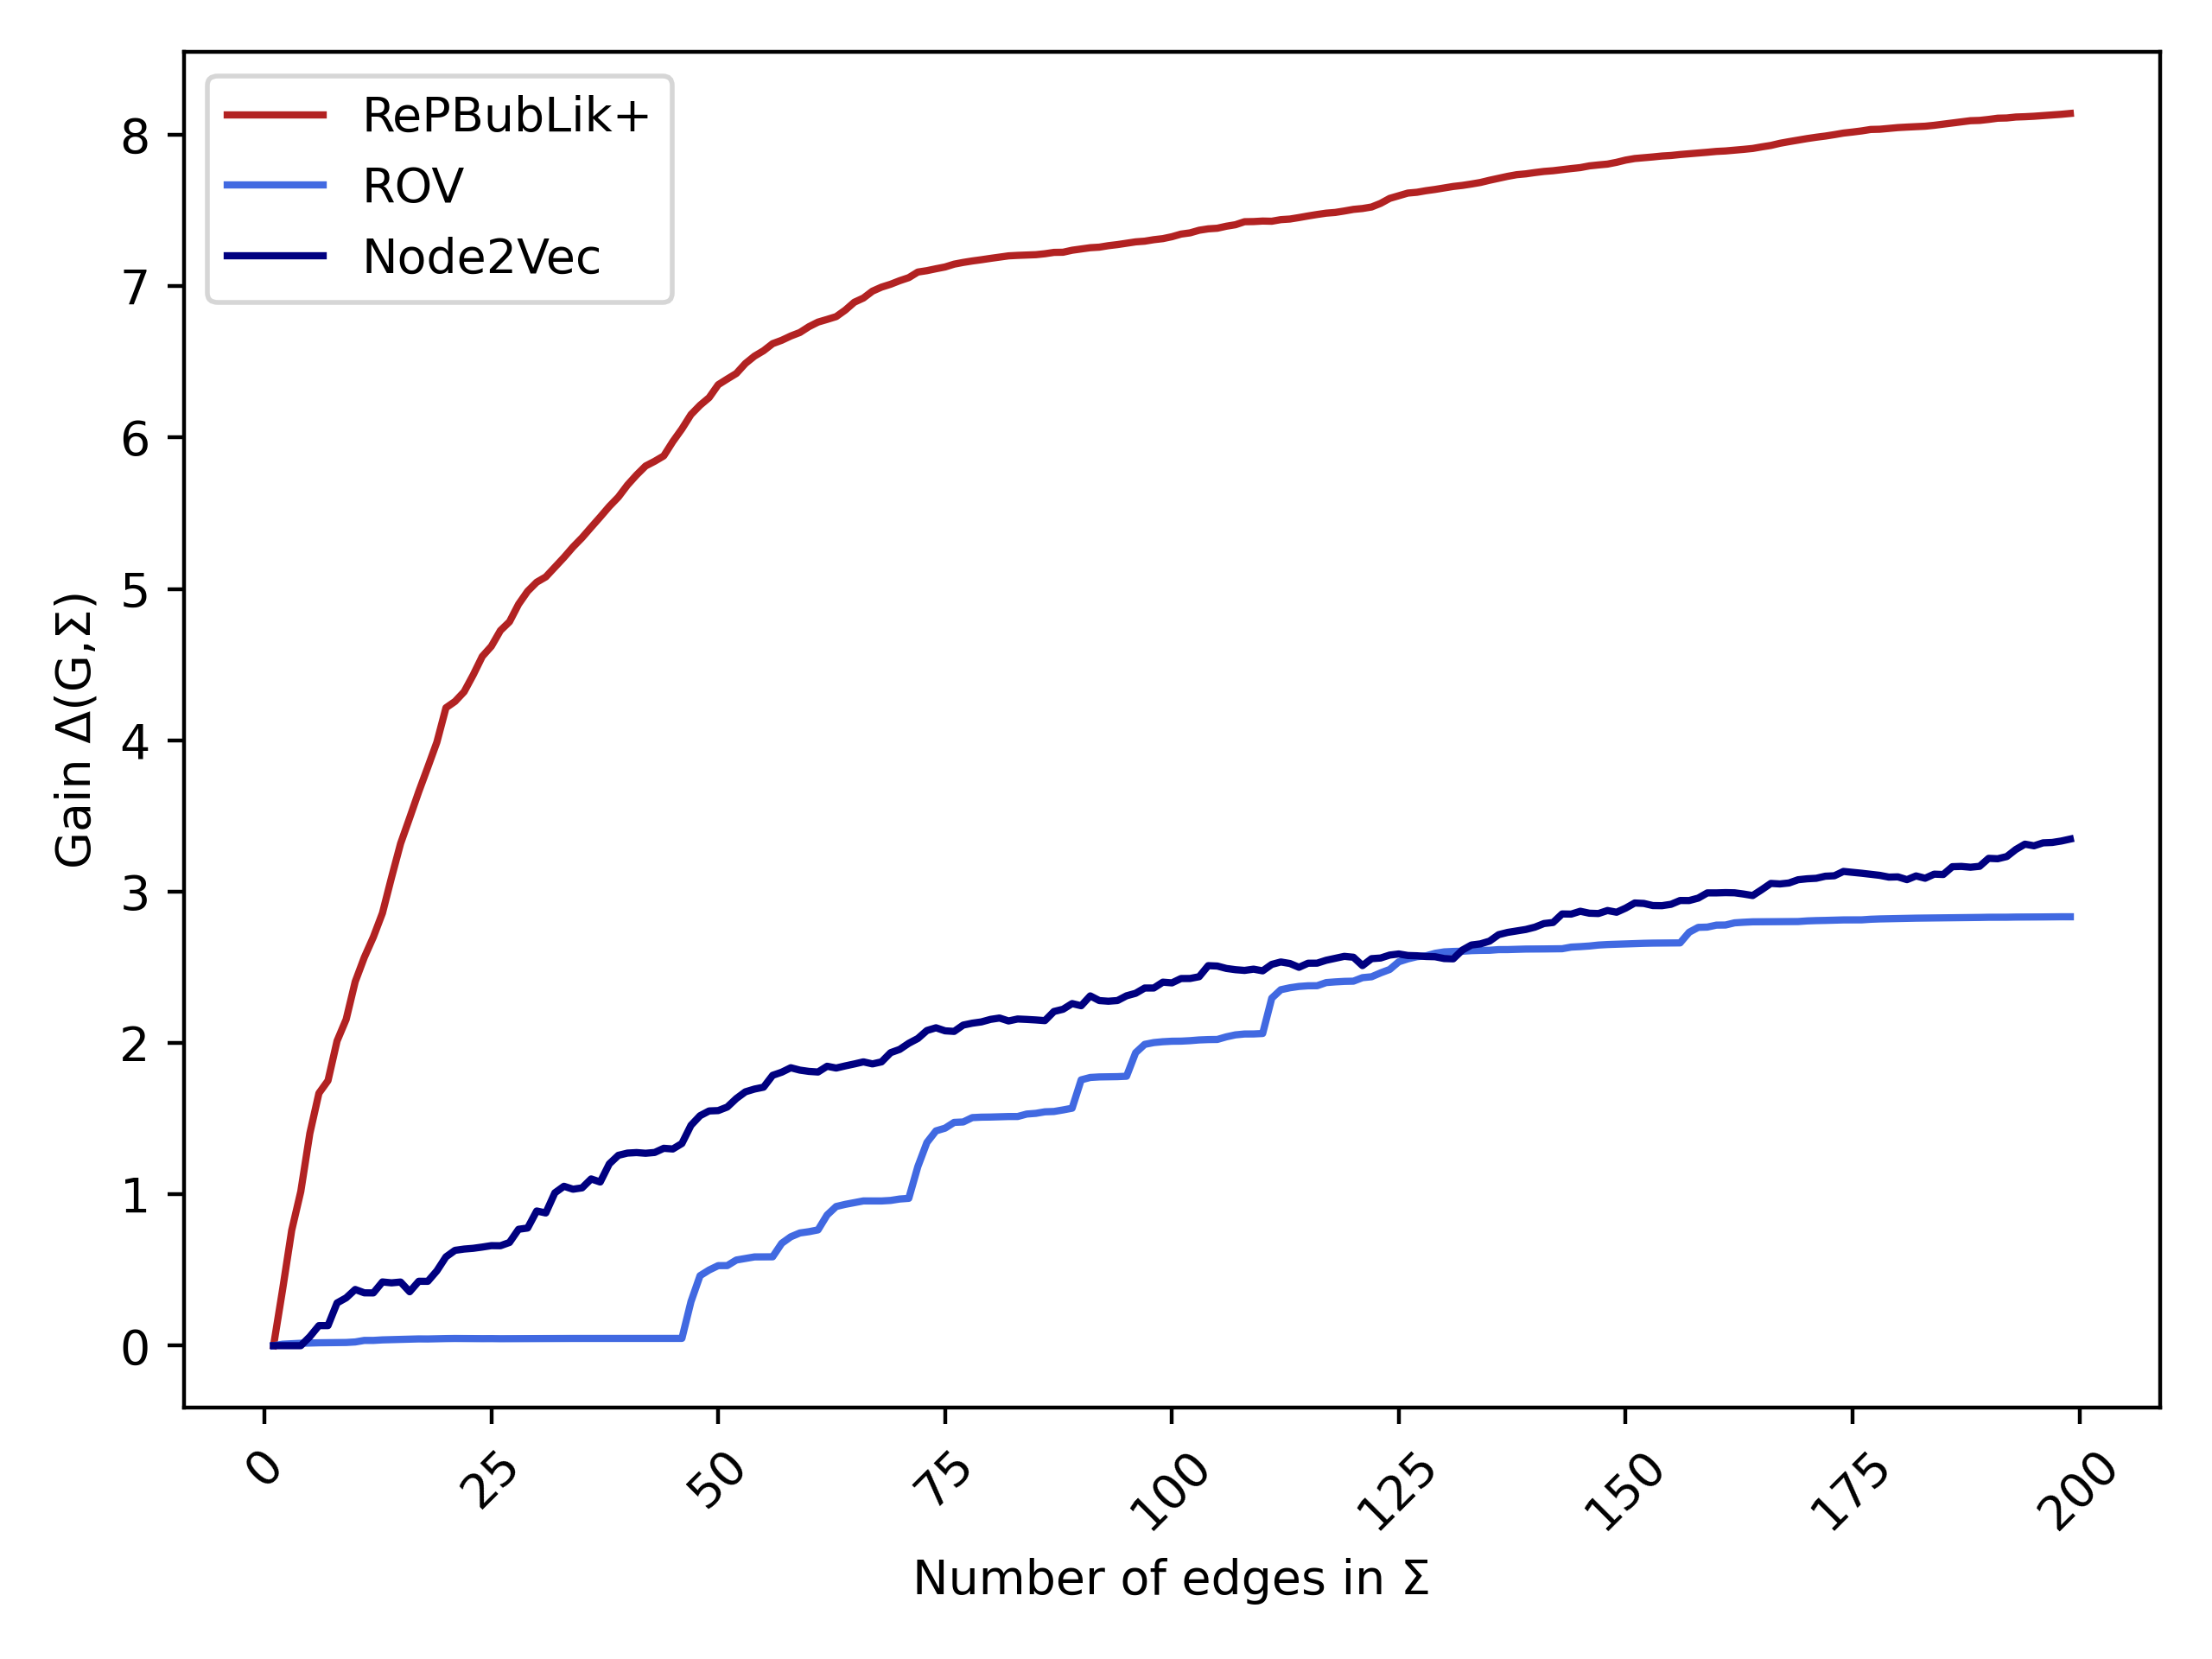
\includegraphics[width=\columnwidth]{10/math_ast_gain_10.png}
    \caption{\emph{MaA}s plot}\label{fig:maas_g_10}
\end{subfigure}
\hspace{0.1\columnwidth}
\begin{subfigure}[b]{0.4\textwidth}
    \centering
    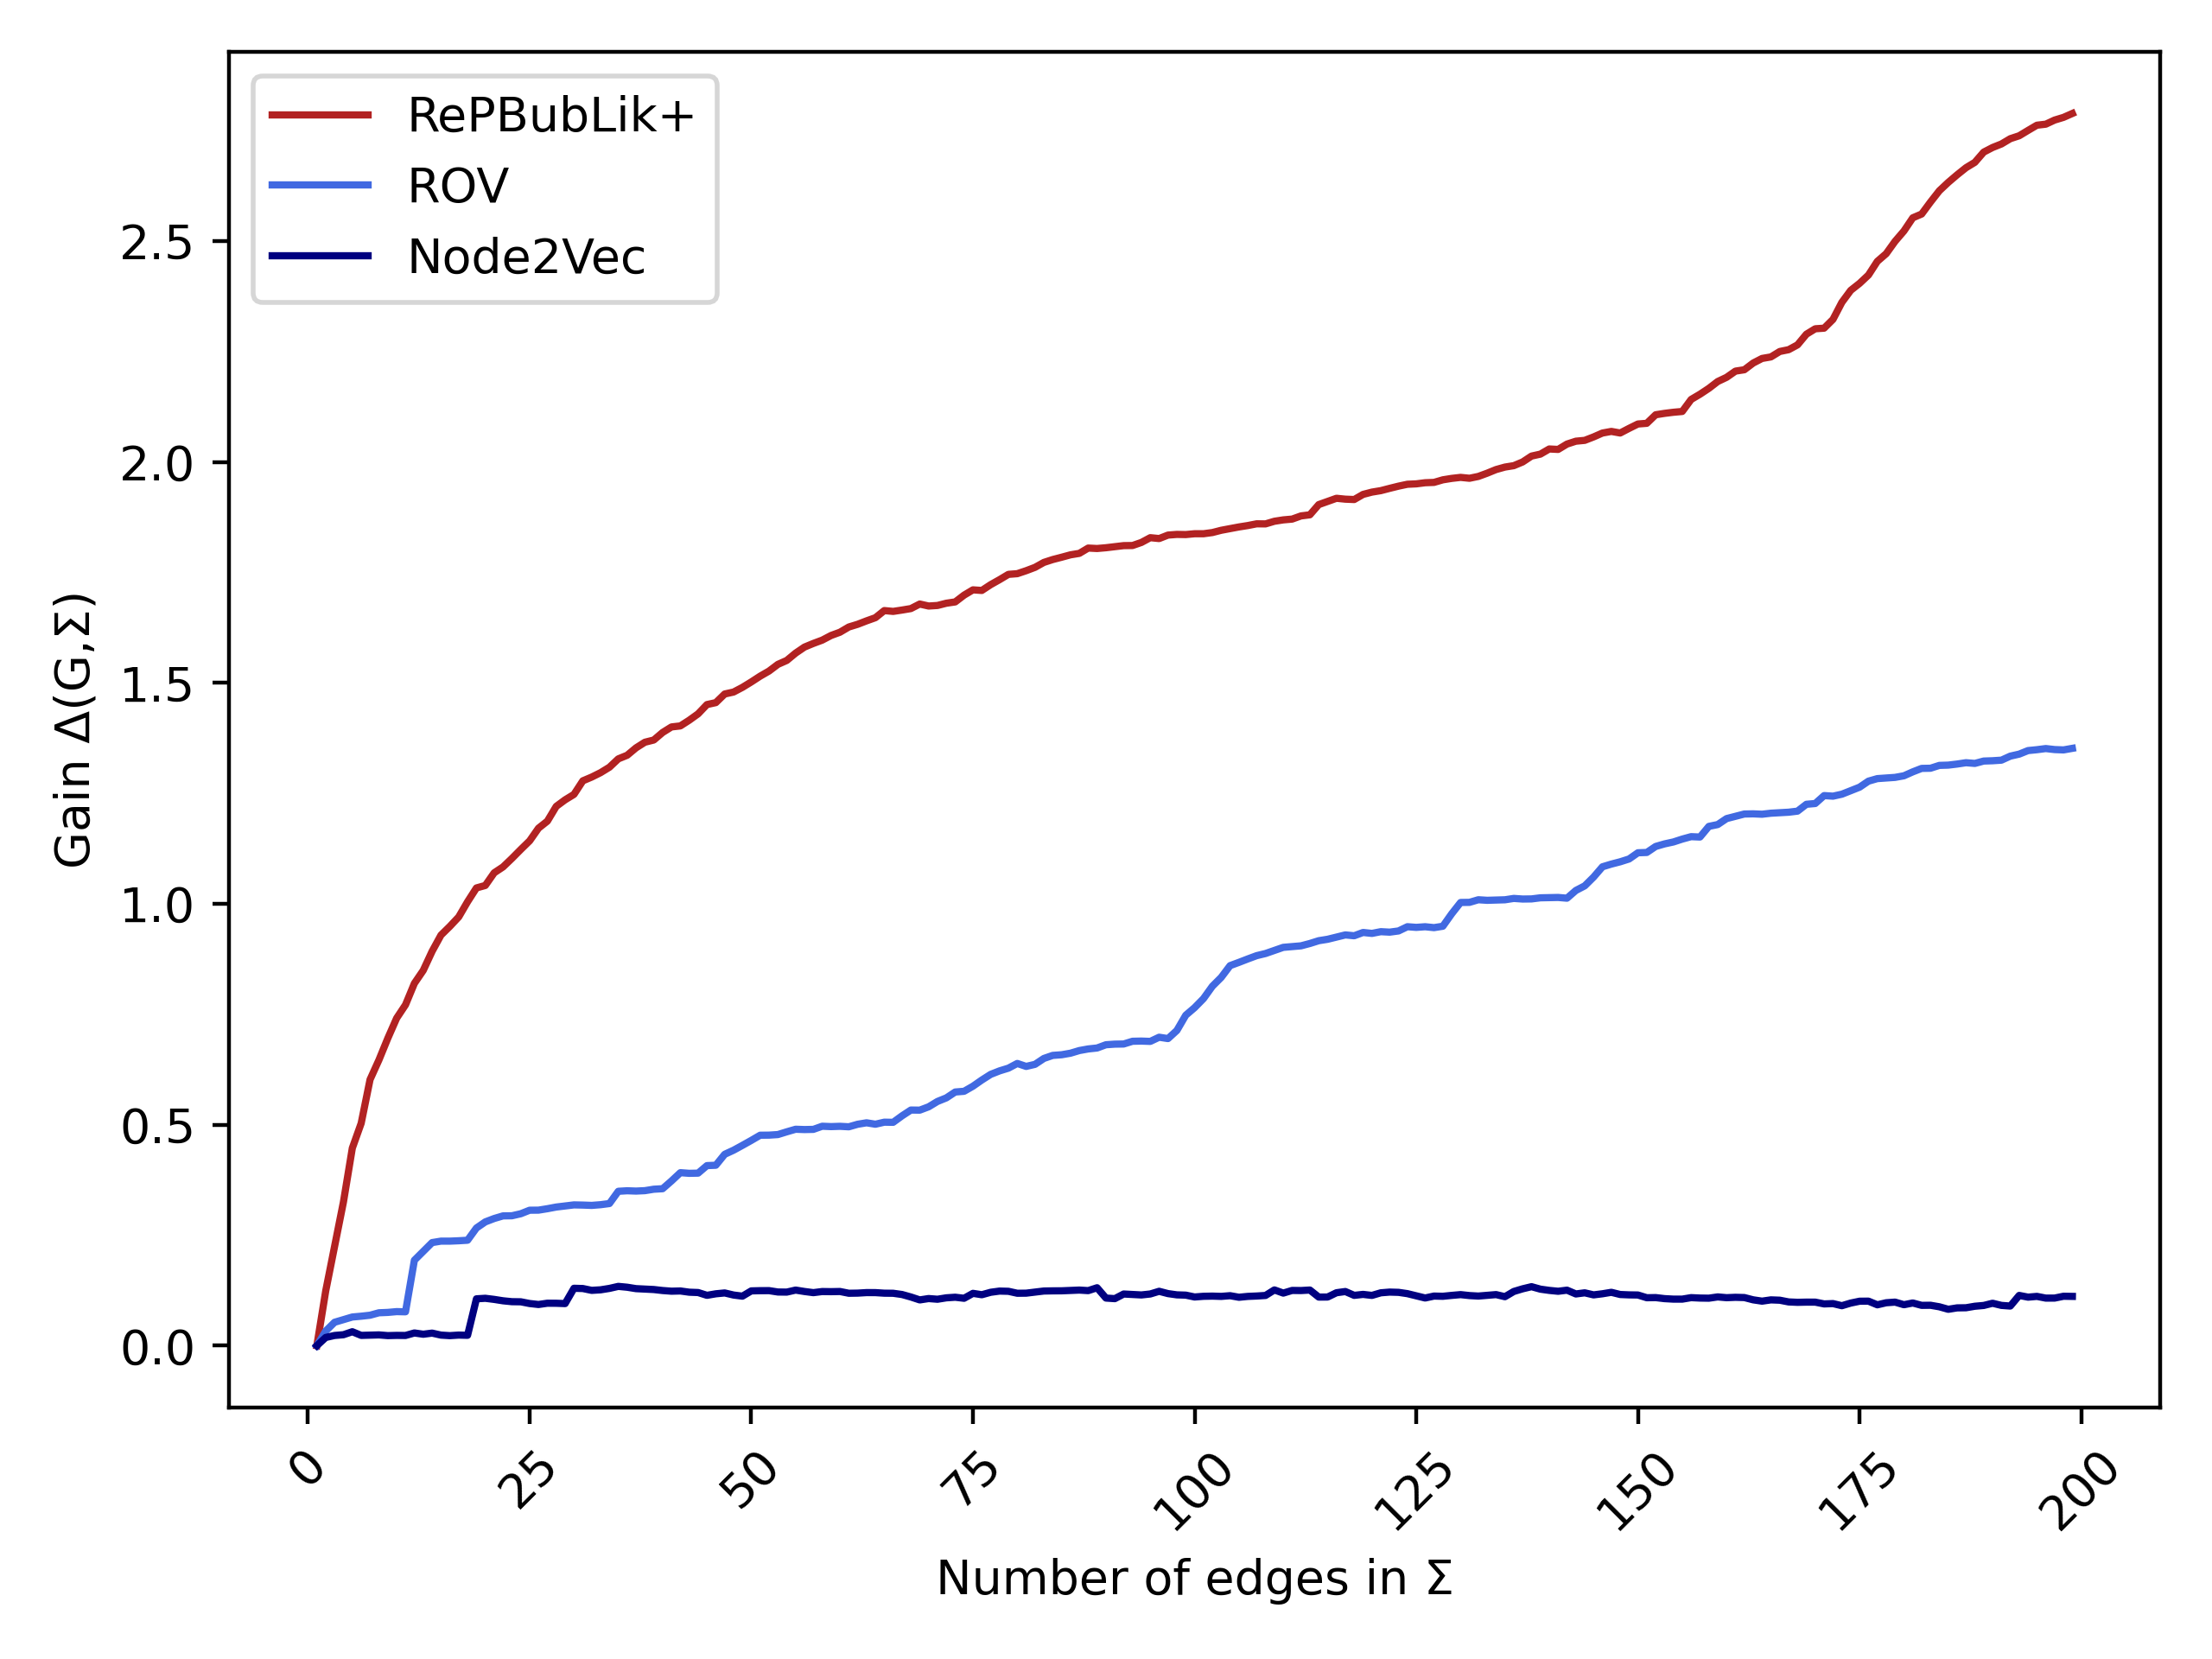
\includegraphics[width=\columnwidth]{10/polblogs_gain_10.png}
    \caption{\emph{PolBlogs} plot}\label{fig:polblogs_g_10}
\end{subfigure}
\caption{Grafici $\Delta(G,\Sigma)$ per $t=10$}
\end{figure}
\newpage
\begin{figure}[!h]
    \centering
\begin{subfigure}[b]{0.4\textwidth}
    \centering
    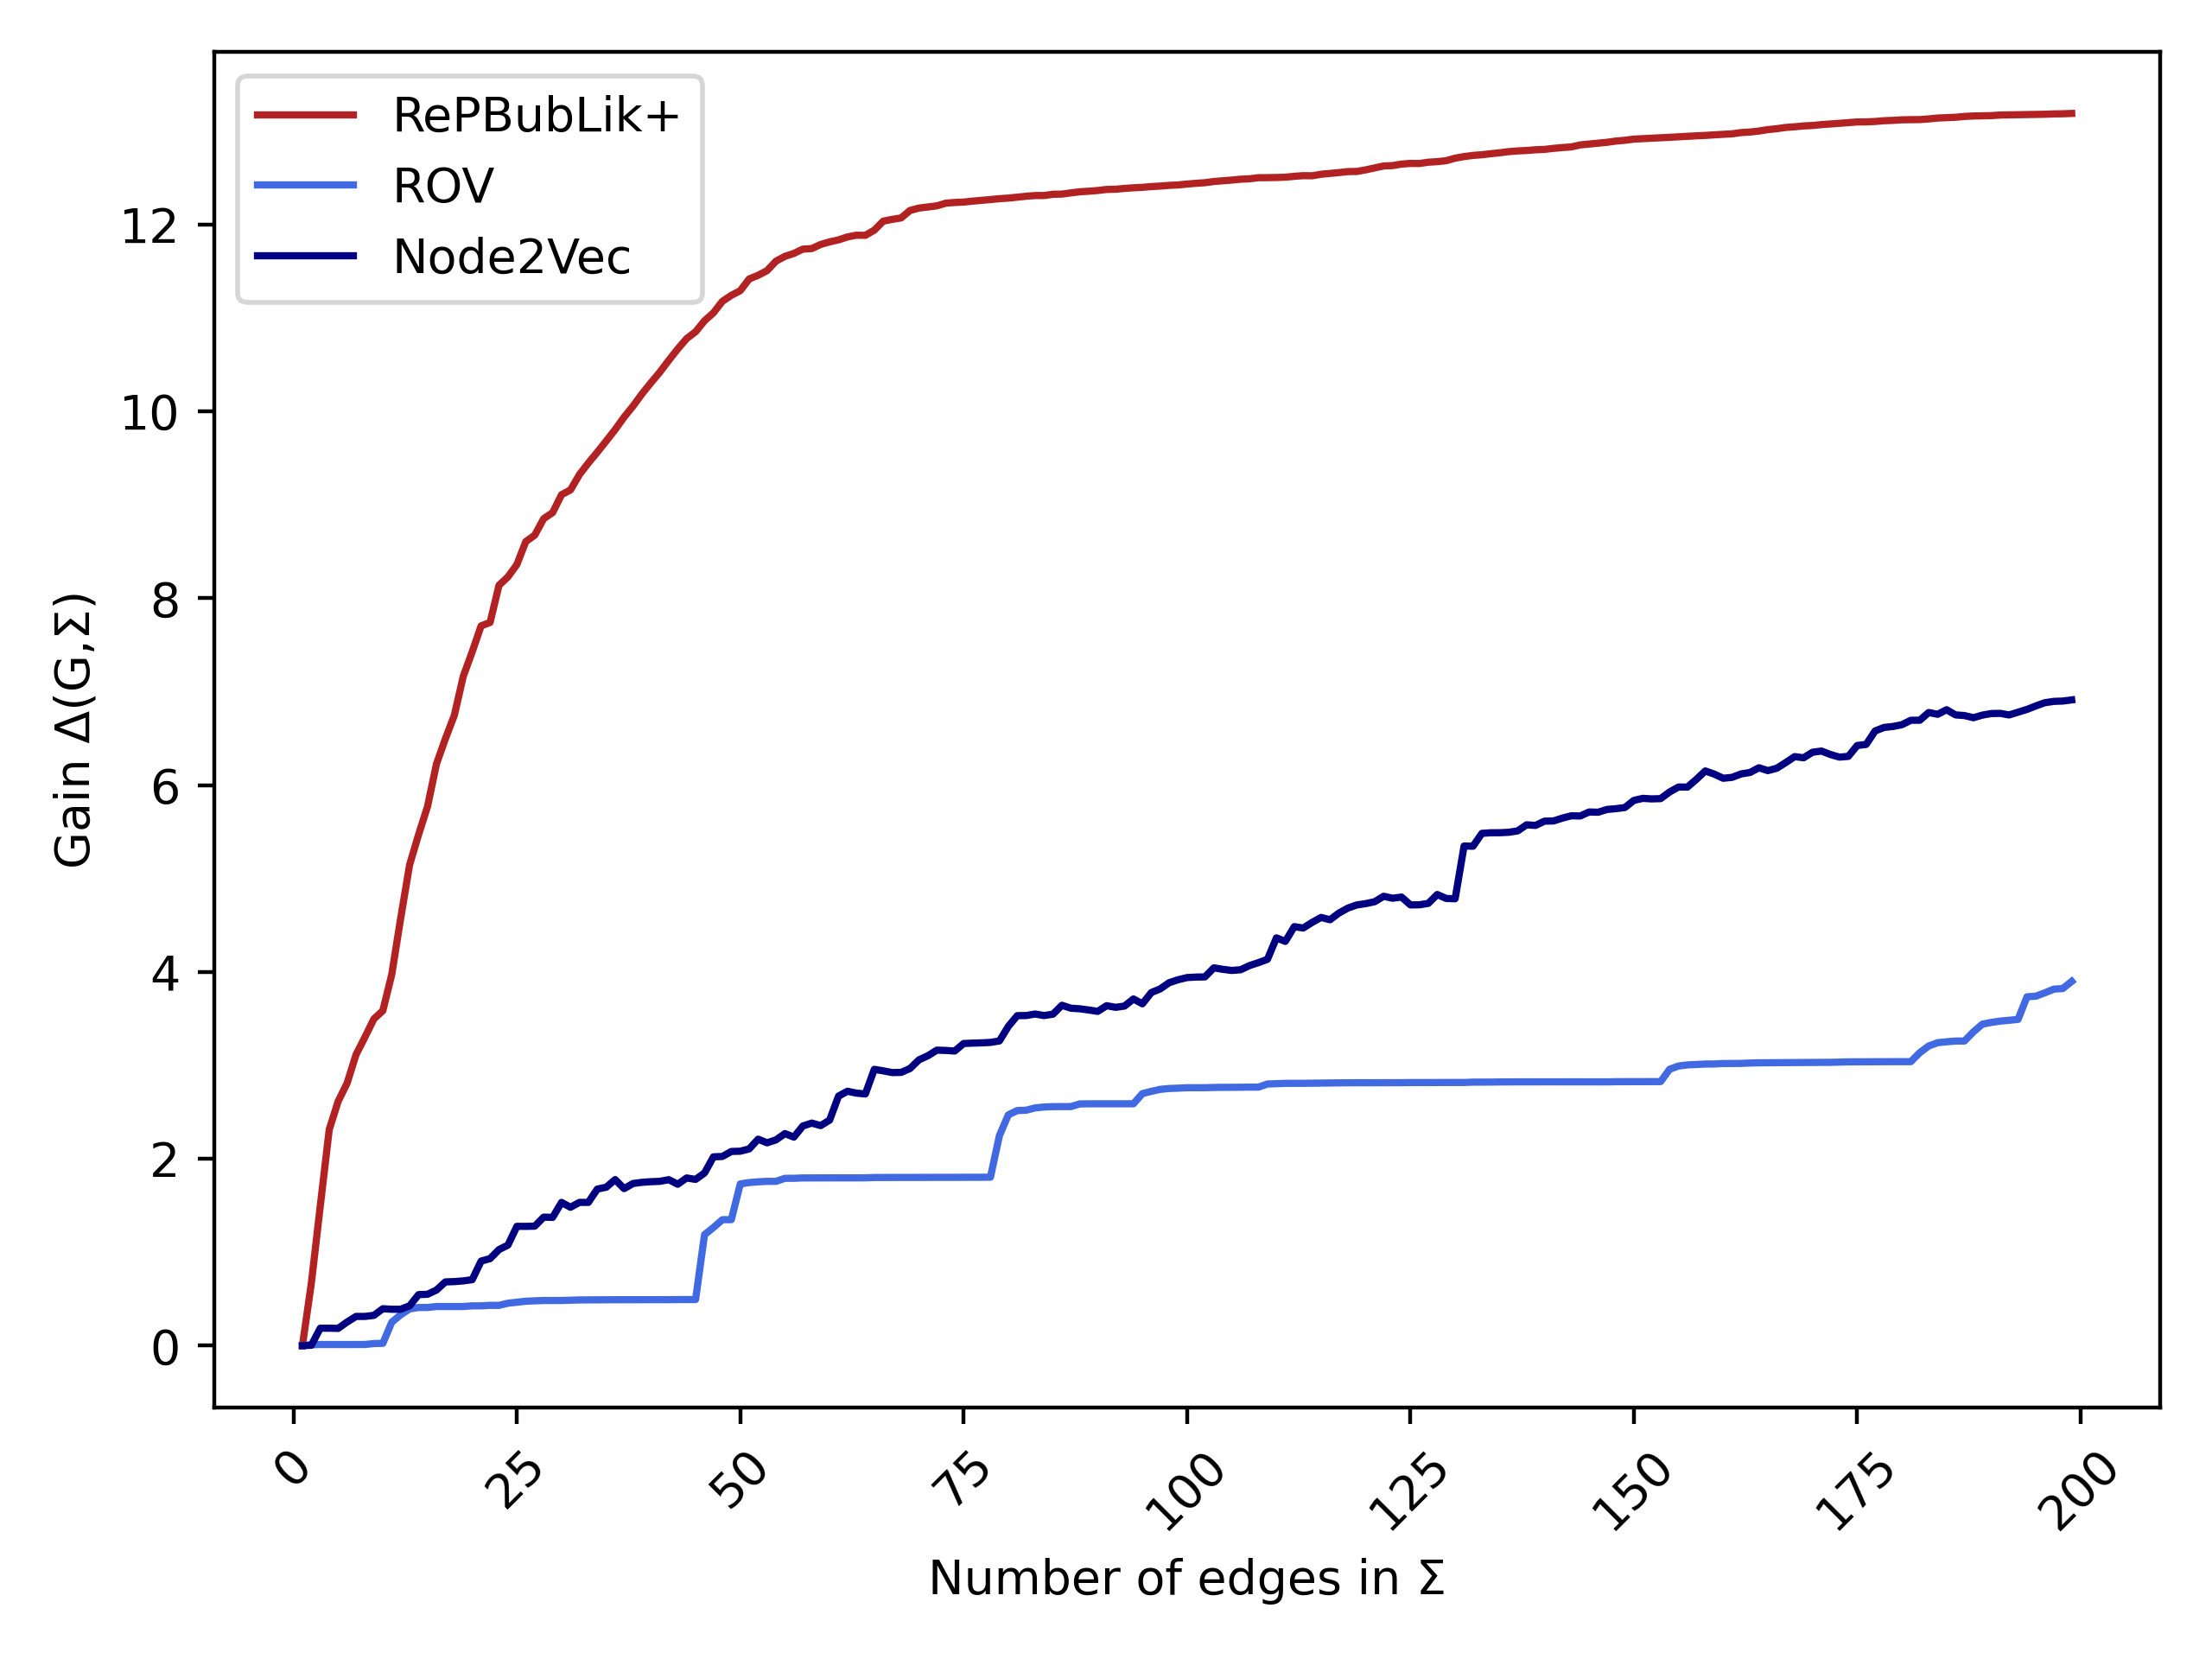
\includegraphics[width=\columnwidth]{15/math_tech_gain_15.png}
    \caption{\emph{MaTe} plot}\label{fig:mate_g_15}
\end{subfigure}
\hspace{0.1\columnwidth}
\begin{subfigure}[b]{0.4\textwidth}
    \centering
    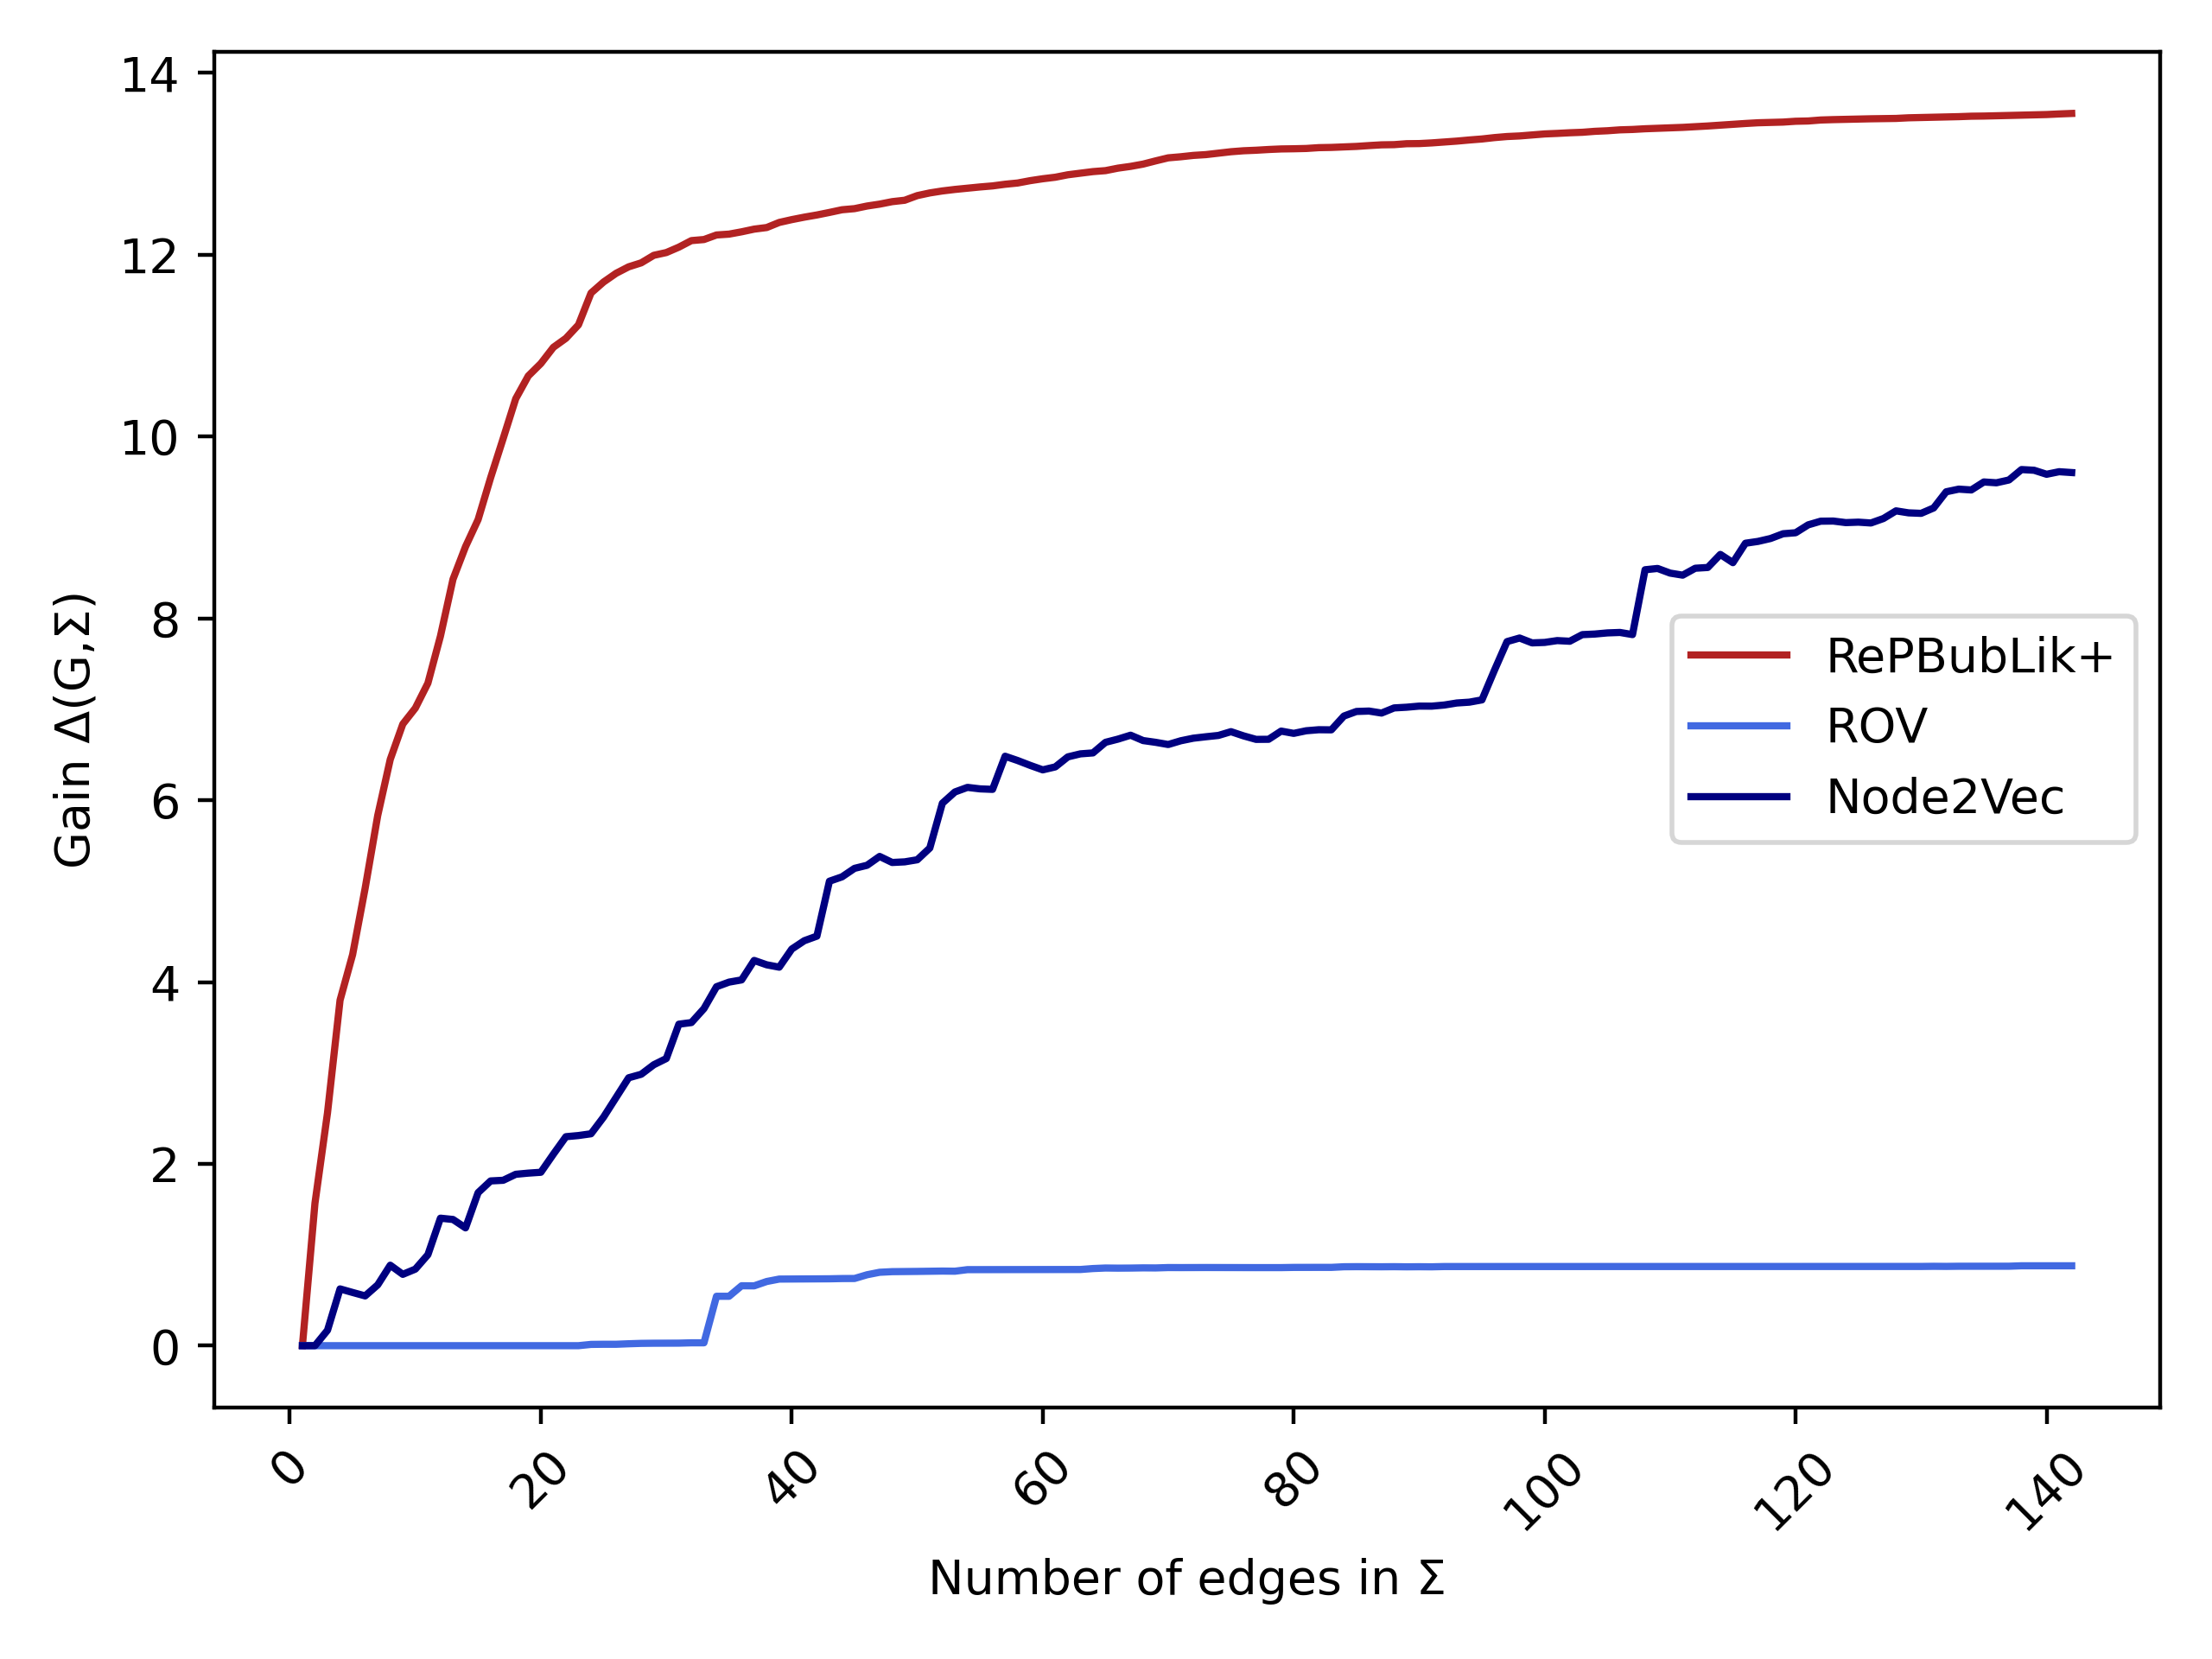
\includegraphics[width=\columnwidth]{15/tech_mil_gain_15.png}
    \caption{\emph{MiHi} plot}\label{fig:mihi_g_15}
\end{subfigure}

\begin{subfigure}[b]{0.4\textwidth}
    \centering
    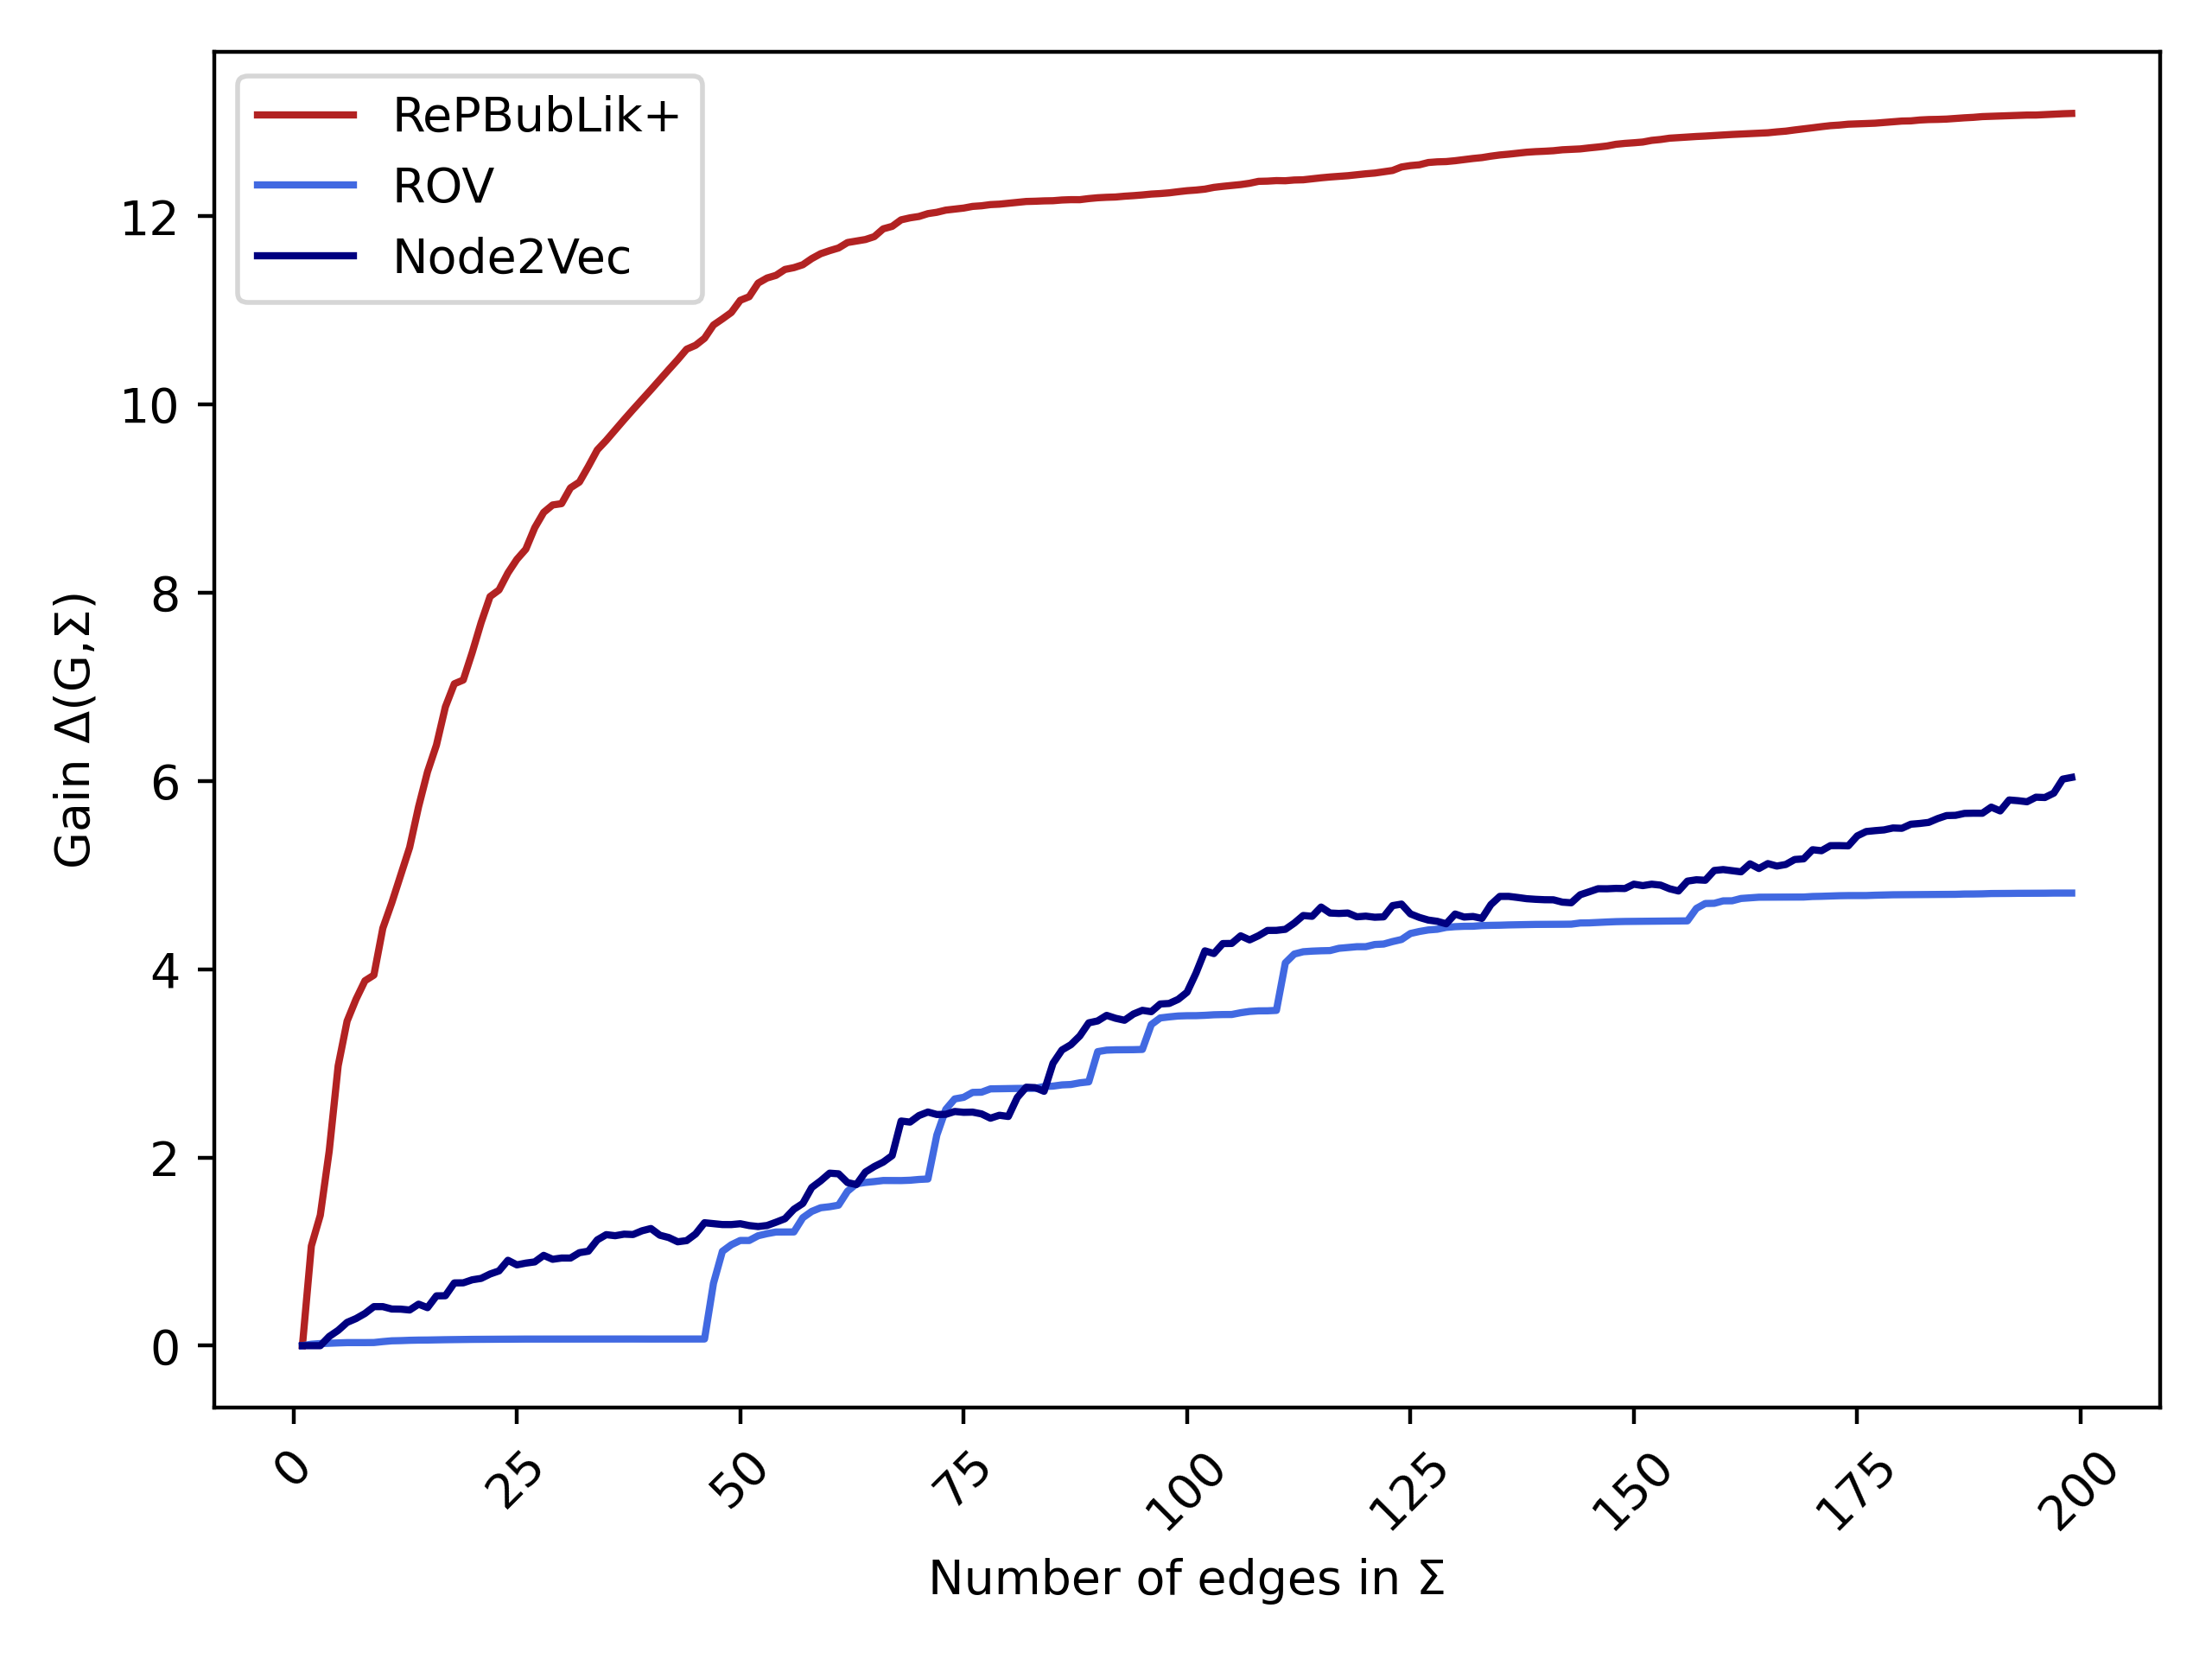
\includegraphics[width=\columnwidth]{15/math_ast_gain_15.png}
    \caption{\emph{MaA}s plot}\label{fig:maas_g_15}
\end{subfigure}
\hspace{0.1\columnwidth}
\begin{subfigure}[b]{0.4\textwidth}
    \centering
    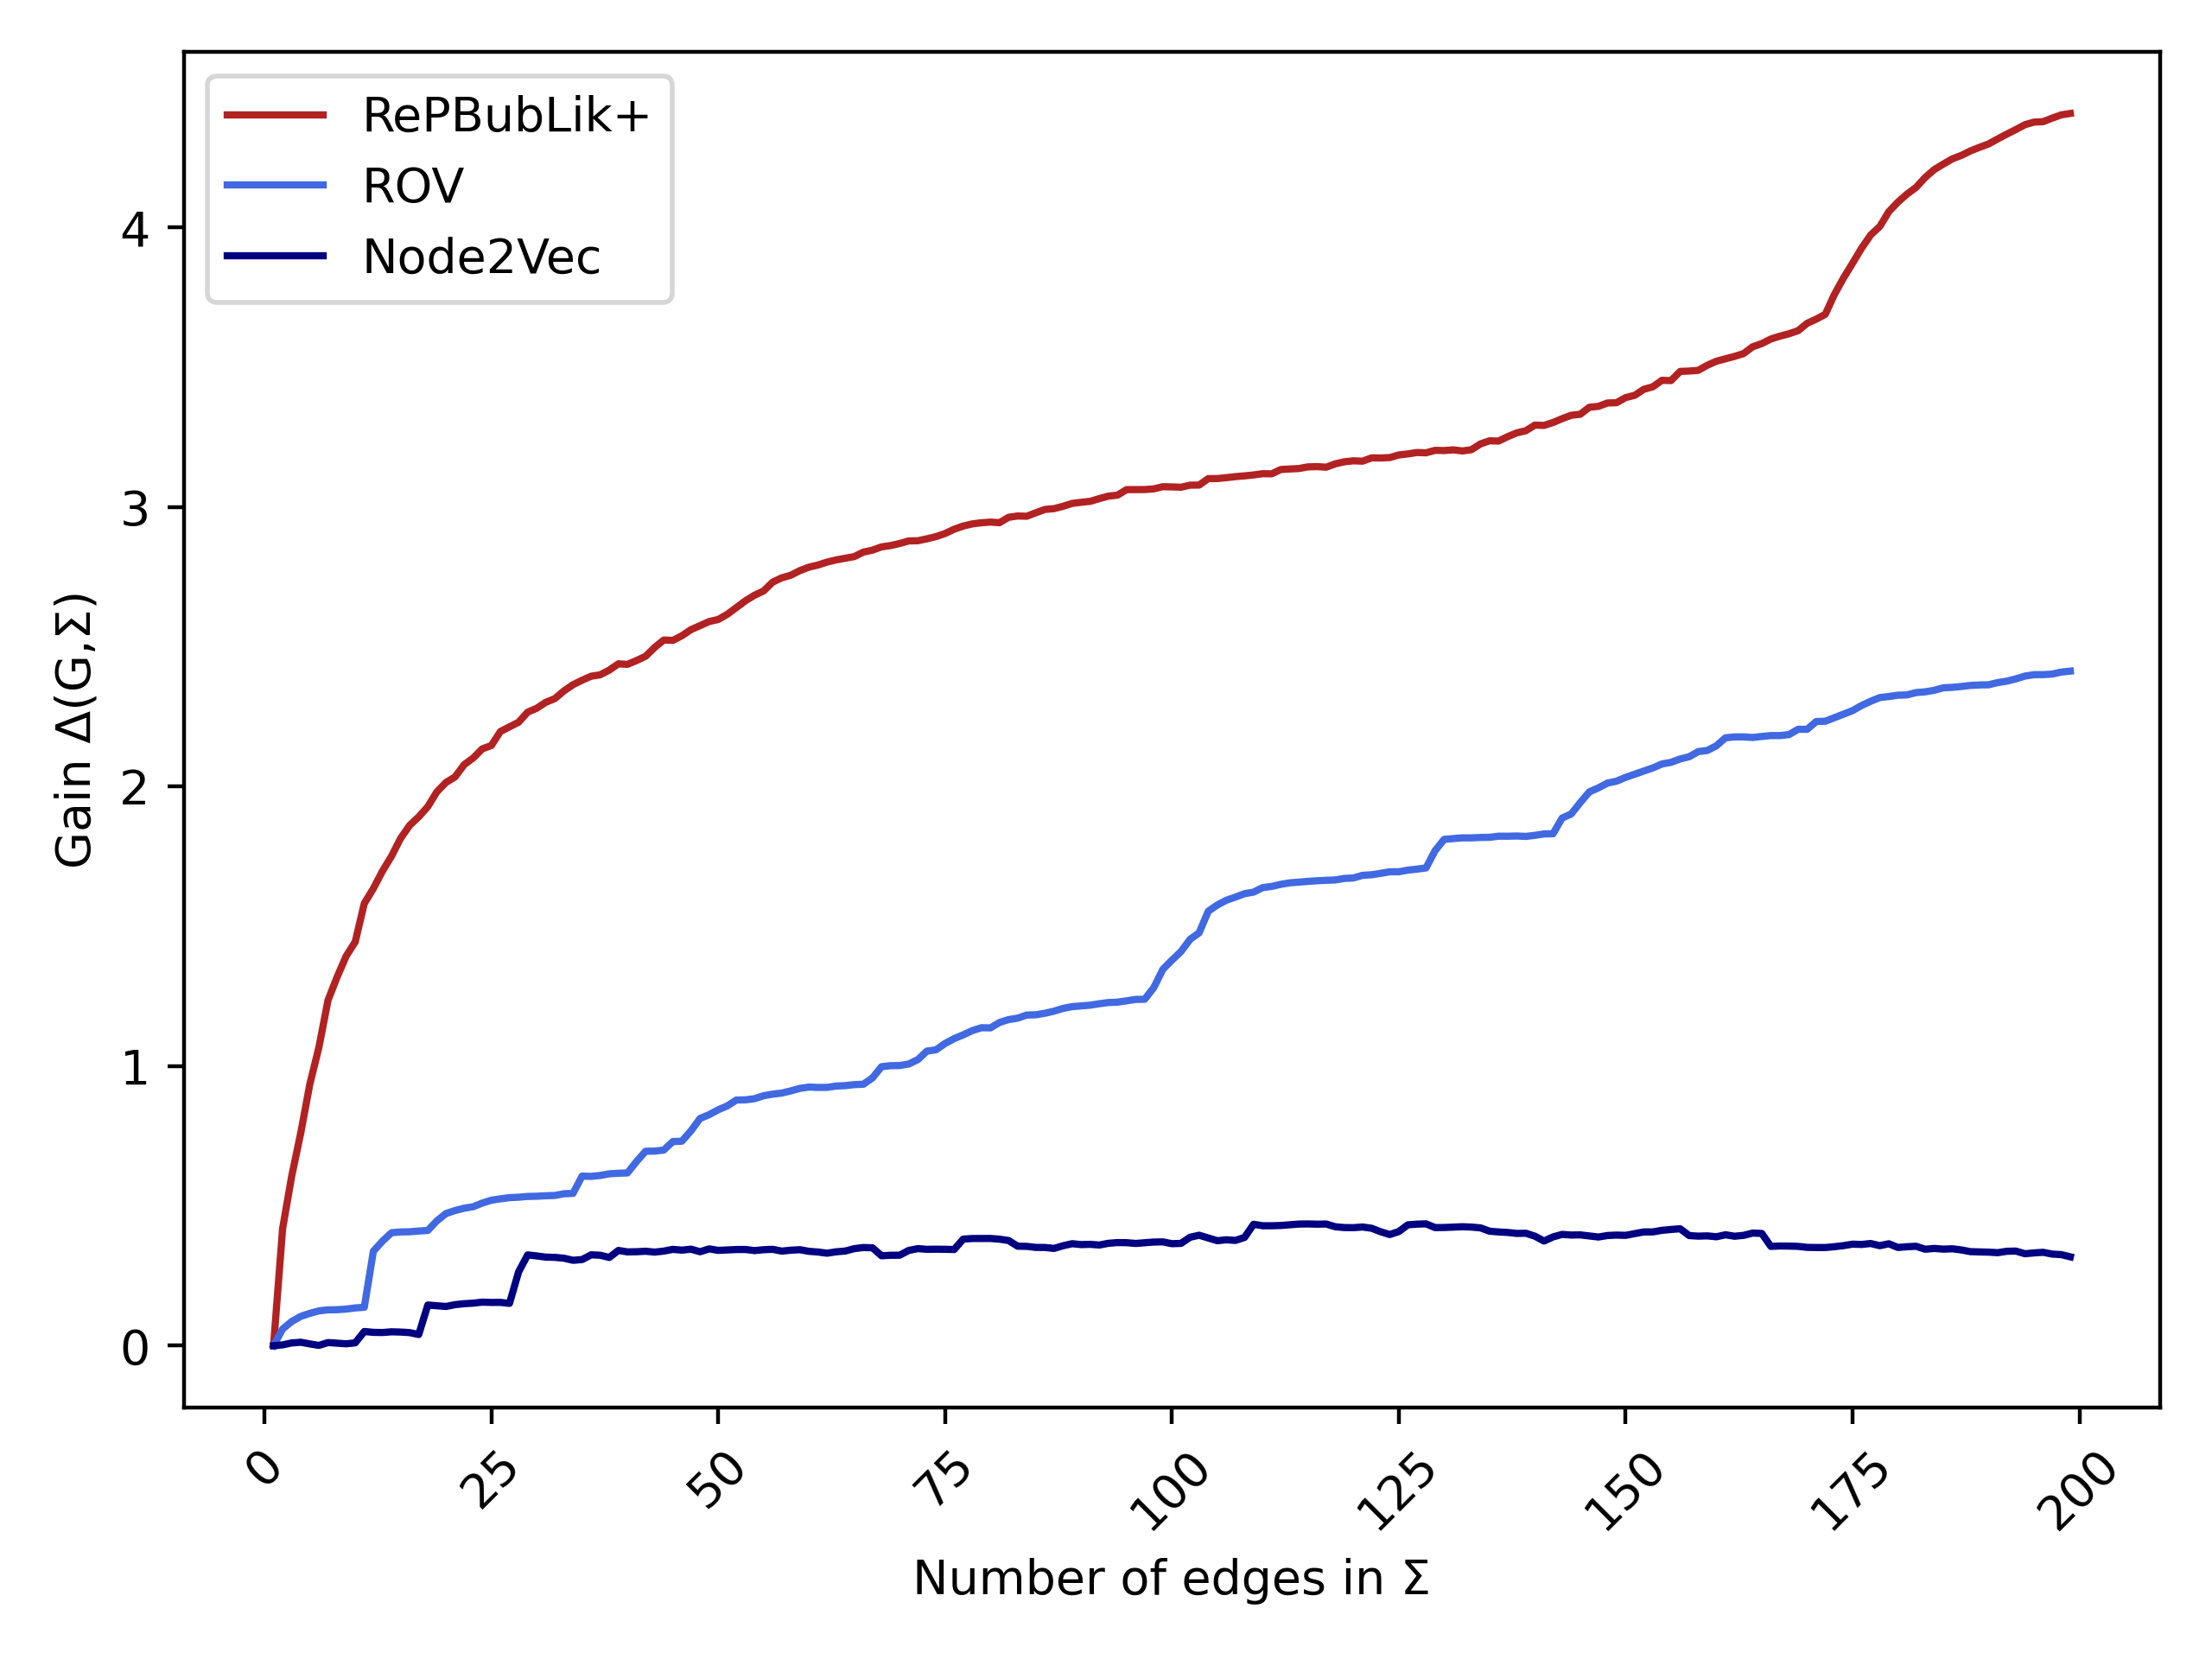
\includegraphics[width=\columnwidth]{15/polblogs_gain_15.png}
    \caption{\emph{PolBlogs} plot}\label{fig:polblogs_g_15}
\end{subfigure}
\caption{Grafici $\Delta(G,\Sigma)$ per $t=15$}
\end{figure}

Dai grafici dei guadagni, si evince che:
\begin{enumerate}
    \item RePBubLik+ è il migliore tra gli algoritmi proposti, in termini di guadagno $\Delta(G,\Sigma)$ rispetto al numero di archi in $\Sigma$.
    \item L'applicazione di RePBubLik+ a grafi di piccole dimensioni (\emph{MaTe}, \emph{MaAs}, \emph{MiHi}) porta ad un guadagno massimo maggiore rispetto a quello ottenuto mediante gli algoritmi ROV e Node2Vec (es. (\emph{MaAs}) ${\Delta_{R+}\over{\Delta_{ROV}}}=2.93$, ${\Delta_{R+}\over{\Delta_{Node2Vec}}}=2.56$ per $k=200,t=10$).
    \item L'applicazione di RePBubLik+ a grafi di medie dimensioni (\emph{PolBlogs}) porta ad un guadagno massimo maggiore rispetto a quello ottenuto mediante gli algoritmi ROV e Node2Vec (es. (\emph{PolBlogs}) ${\Delta_{R+}\over{\Delta_{ROV}}}=2.34$, ${\Delta_{R+}\over{\Delta_{Node2Vec}}}=18.67$ per  $k=200,t=10$).
    \item RePBubLik+ risulta essere il miglior algoritmo in quanto per un numero ridotto di archi riporta un notevole guadagno: nei grafici sovrastanti, la curva dell'algoritmo RePBubLik+ cresce molto rapidamente per valori piccoli di $k$, raggiungendo una plateau per un certo valore di $\Delta(G,\Sigma)$.
            Questo, dal punto di vista pratico, è molto interessante perchè permette con pochi archi aggiuntivi di ridurre notevolmente la polarizzazione in grafi simili a quelli presi in esame (es. (\emph{MaTe}) ${\Delta_{R+}\over{\Delta_{ROV}}}=7.45$, ${\Delta_{R+}\over{\Delta_{Node2Vec}}}=3.35$ per $k=50,t=10$).
    \item Le considerazioni fatte nei punti precedenti sono generalmente valide, per qualsiasi valore di $t$ e qualsiasi grafo. Valutando i guadagni dei grafi anche in termini di RW massimo, si può notare che per valori di $t$ maggiori, RePBubLik+ raggiunge il plateau con un numero inferiore d'archi (es. (\emph{MaTe}) $\Delta_{R+}=2$ per $k=50, t=5$,  $\Delta_{R+}=6.75$ per $k=50,t=10$, $\Delta_{R+}=11.5$ per $k=50,t=15$).
\end{enumerate}
\subsection{Bias strutturale $\rho(G)$}
L'ultima metrica che viene anlizzata è il il bias $\rho(G)$ (\ref{REP:bias}) in relazione al numero 
degli archi aggiunti al grafo $G$. Lo studio di questa misura è interessante, in quanto permette di valutare il cambiamento della polarizzazione del grafo $G$.
\\
Di seguito i bias per ciascun grafo e per ciascun valore di $t$.

\begin{figure}[!h]
    \centering
\begin{subfigure}[b]{0.4\textwidth}
    \centering
    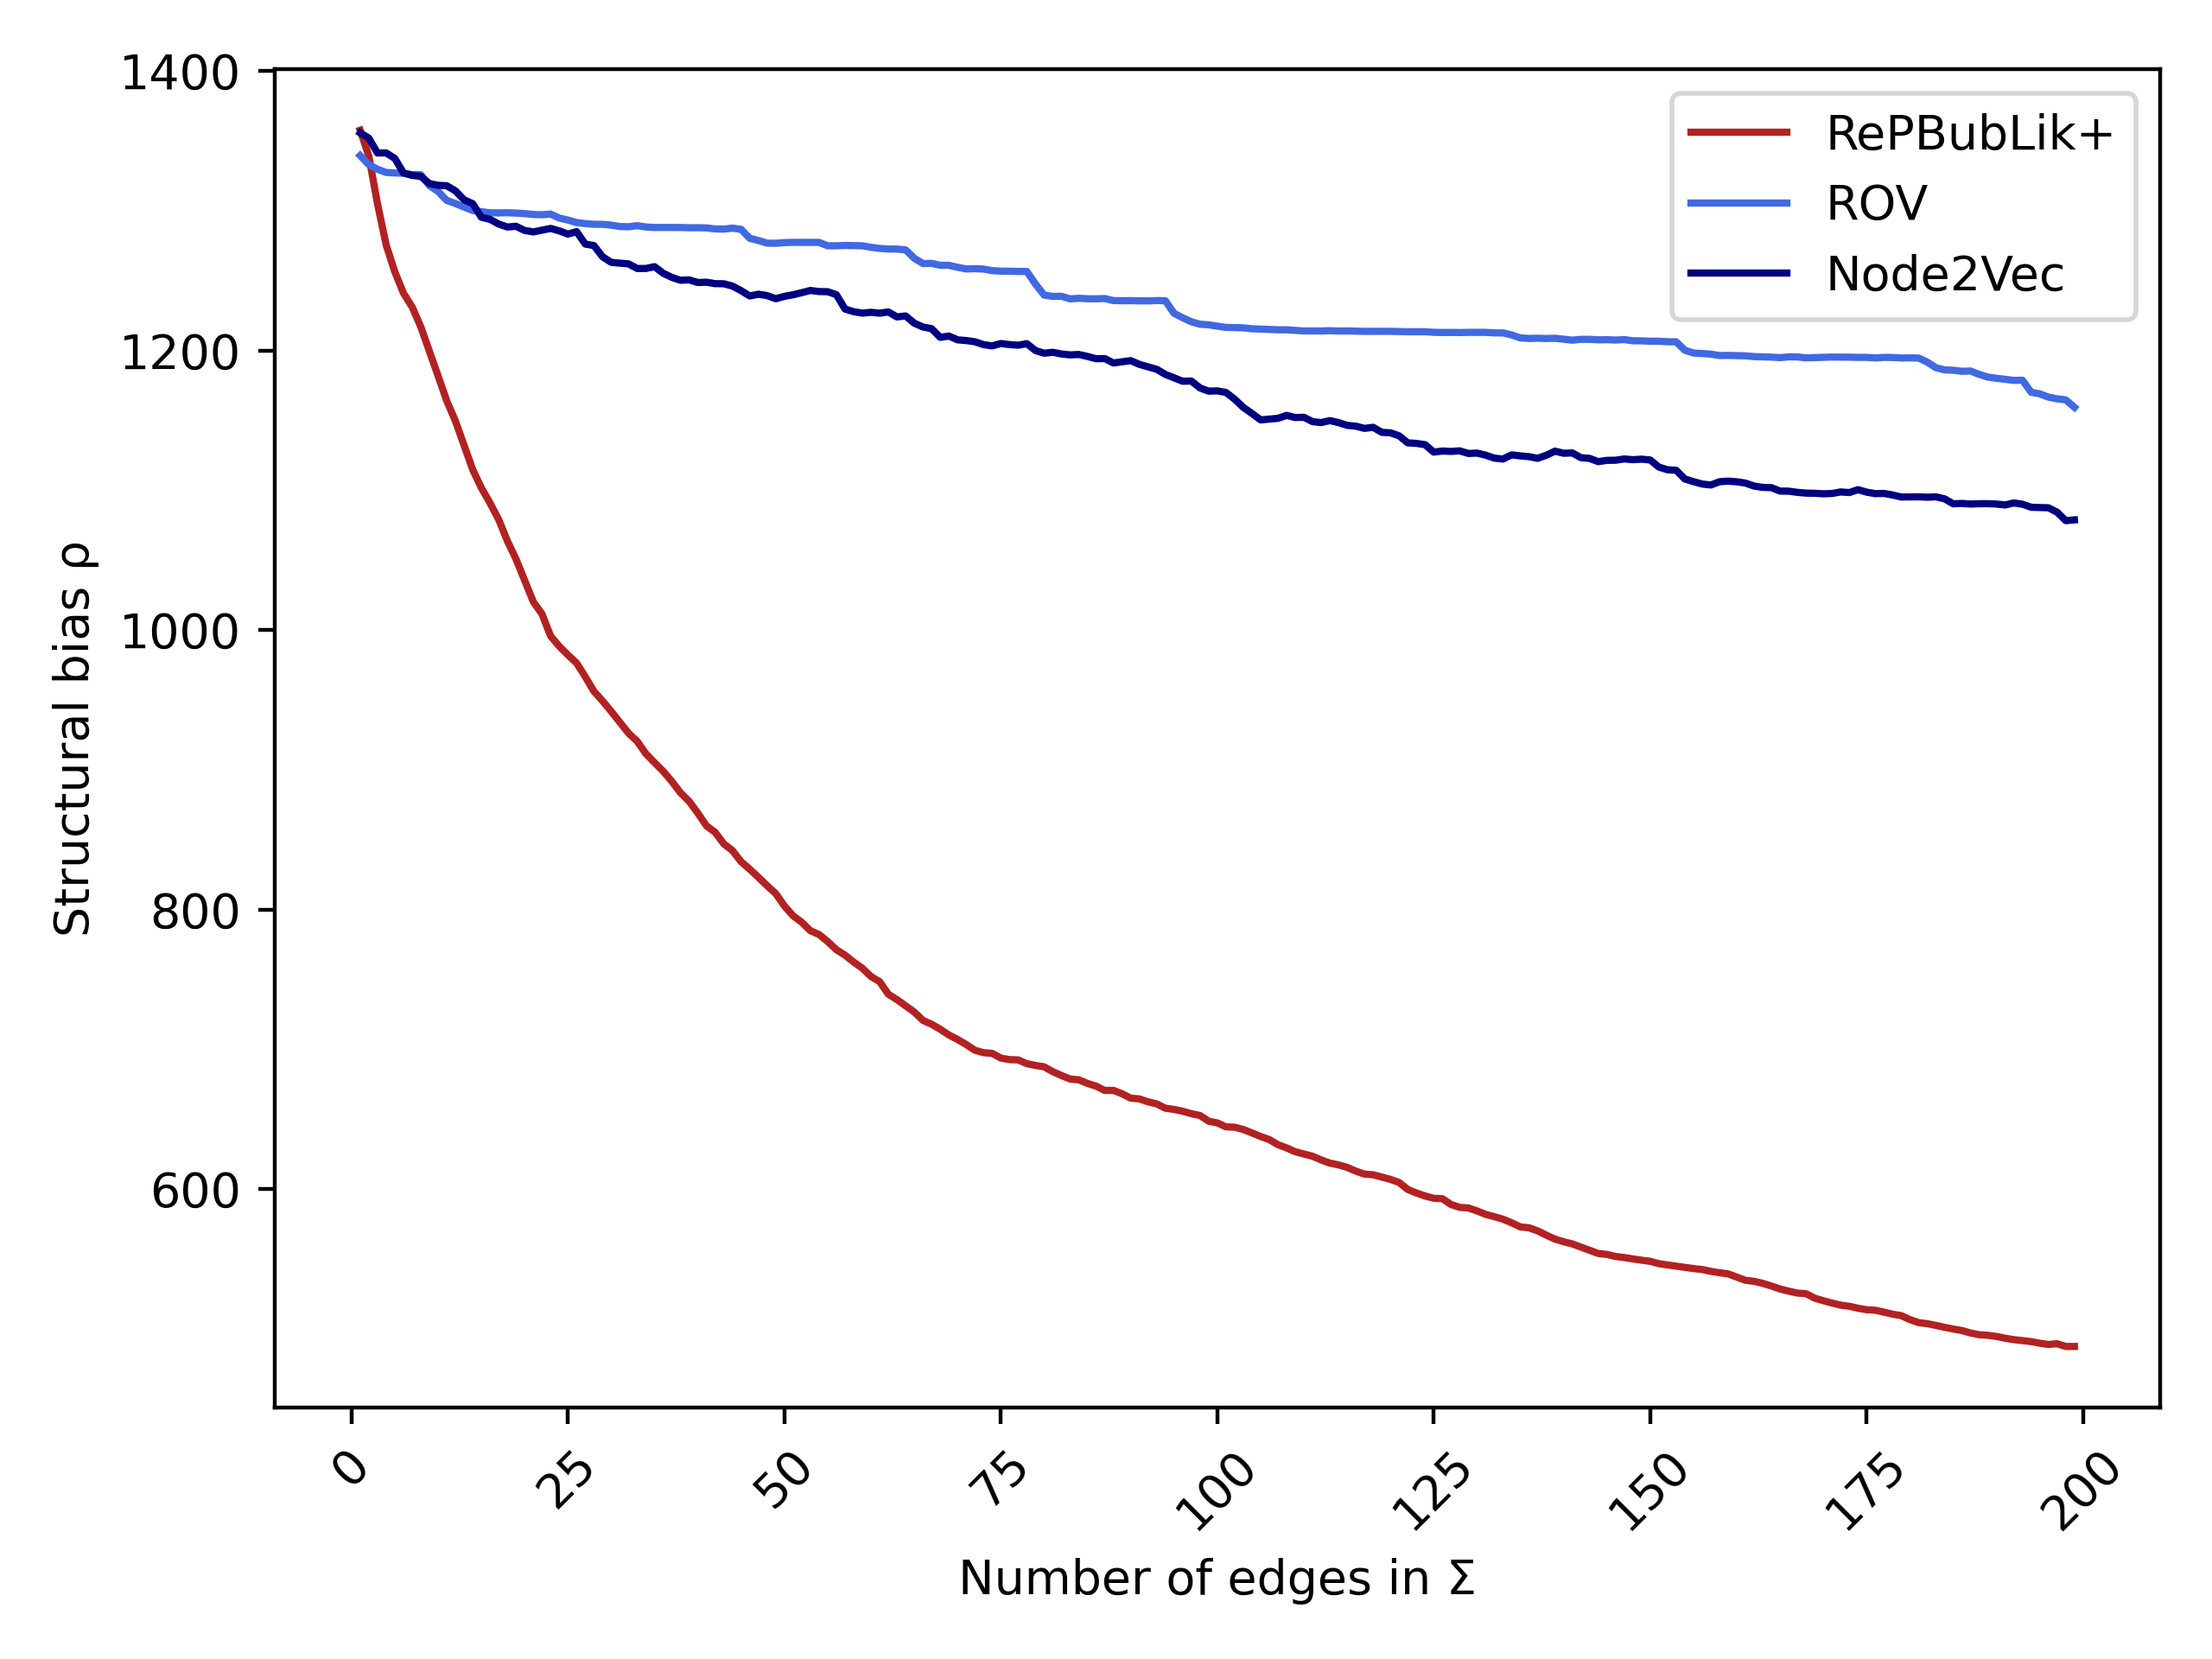
\includegraphics[width=\columnwidth]{5/math_tech_bias_5.png}
    \caption{\emph{MaTe} plot}\label{fig:mate_b_5}
\end{subfigure}
\hspace{0.1\columnwidth}
\begin{subfigure}[b]{0.4\textwidth}
    \centering
    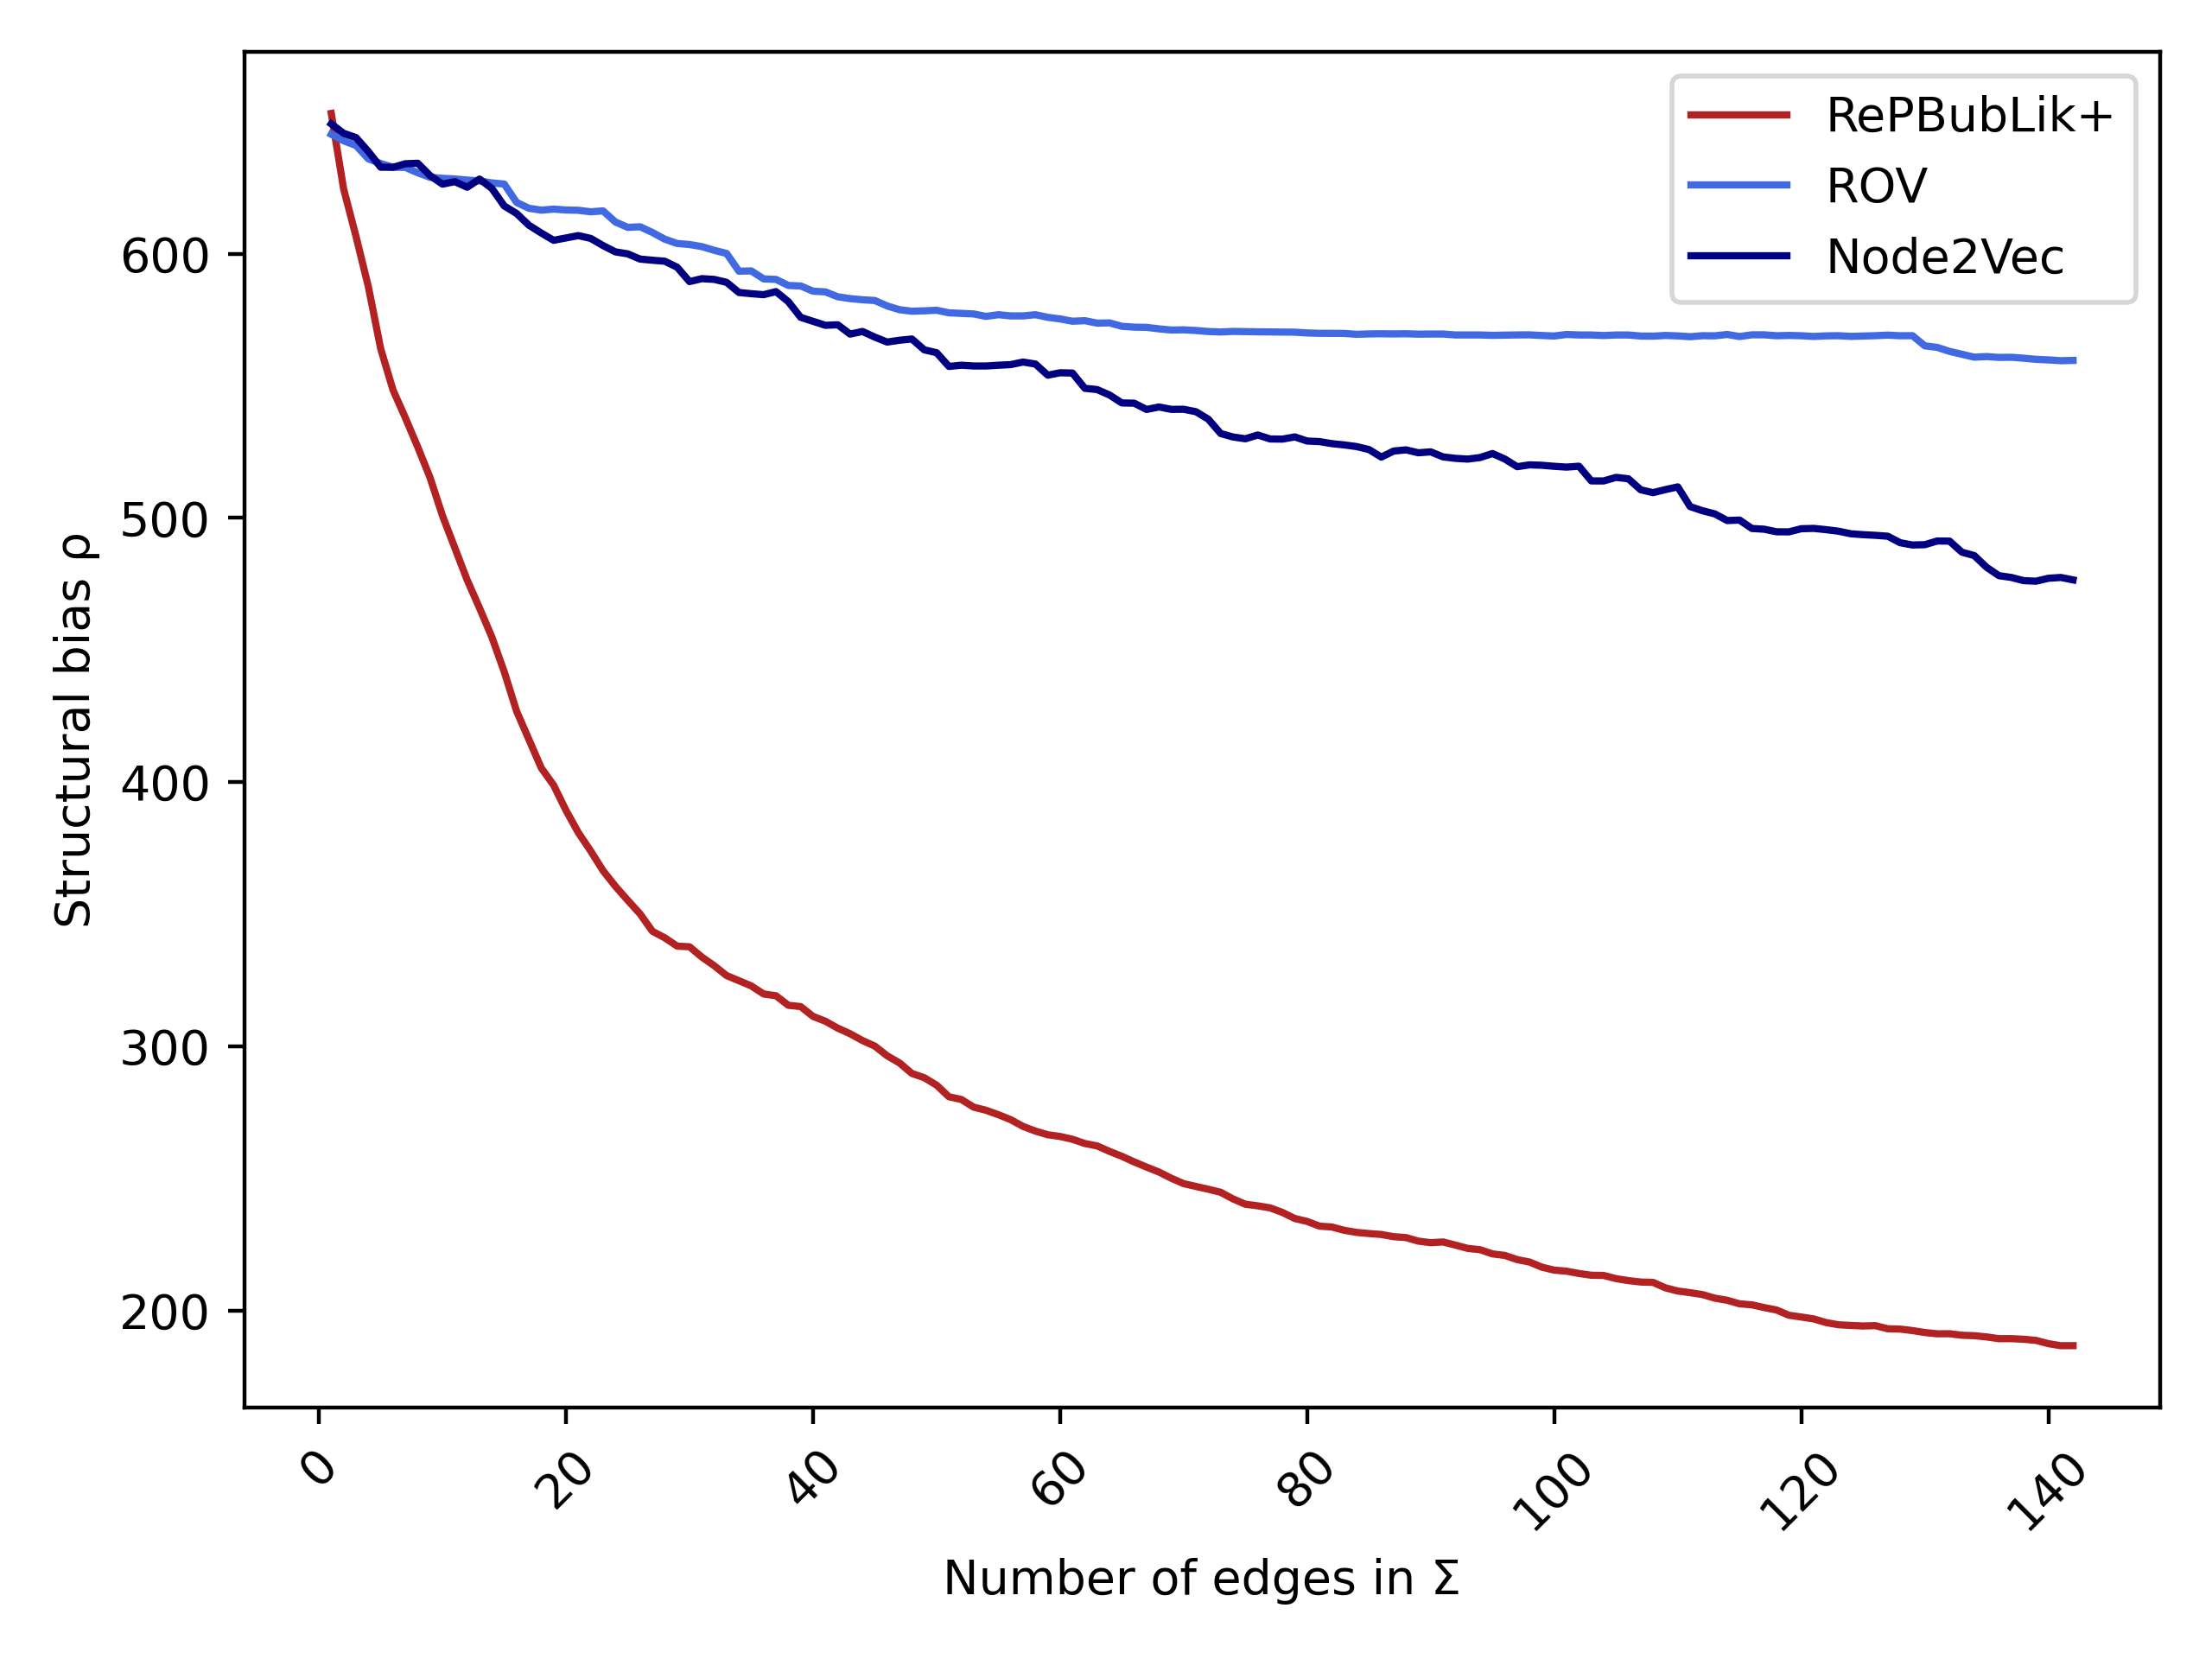
\includegraphics[width=\columnwidth]{5/tech_mil_bias_5.png}
    \caption{\emph{MiHi} plot}\label{fig:mihi_b_5}
\end{subfigure}

\begin{subfigure}[b]{0.4\textwidth}
    \centering
    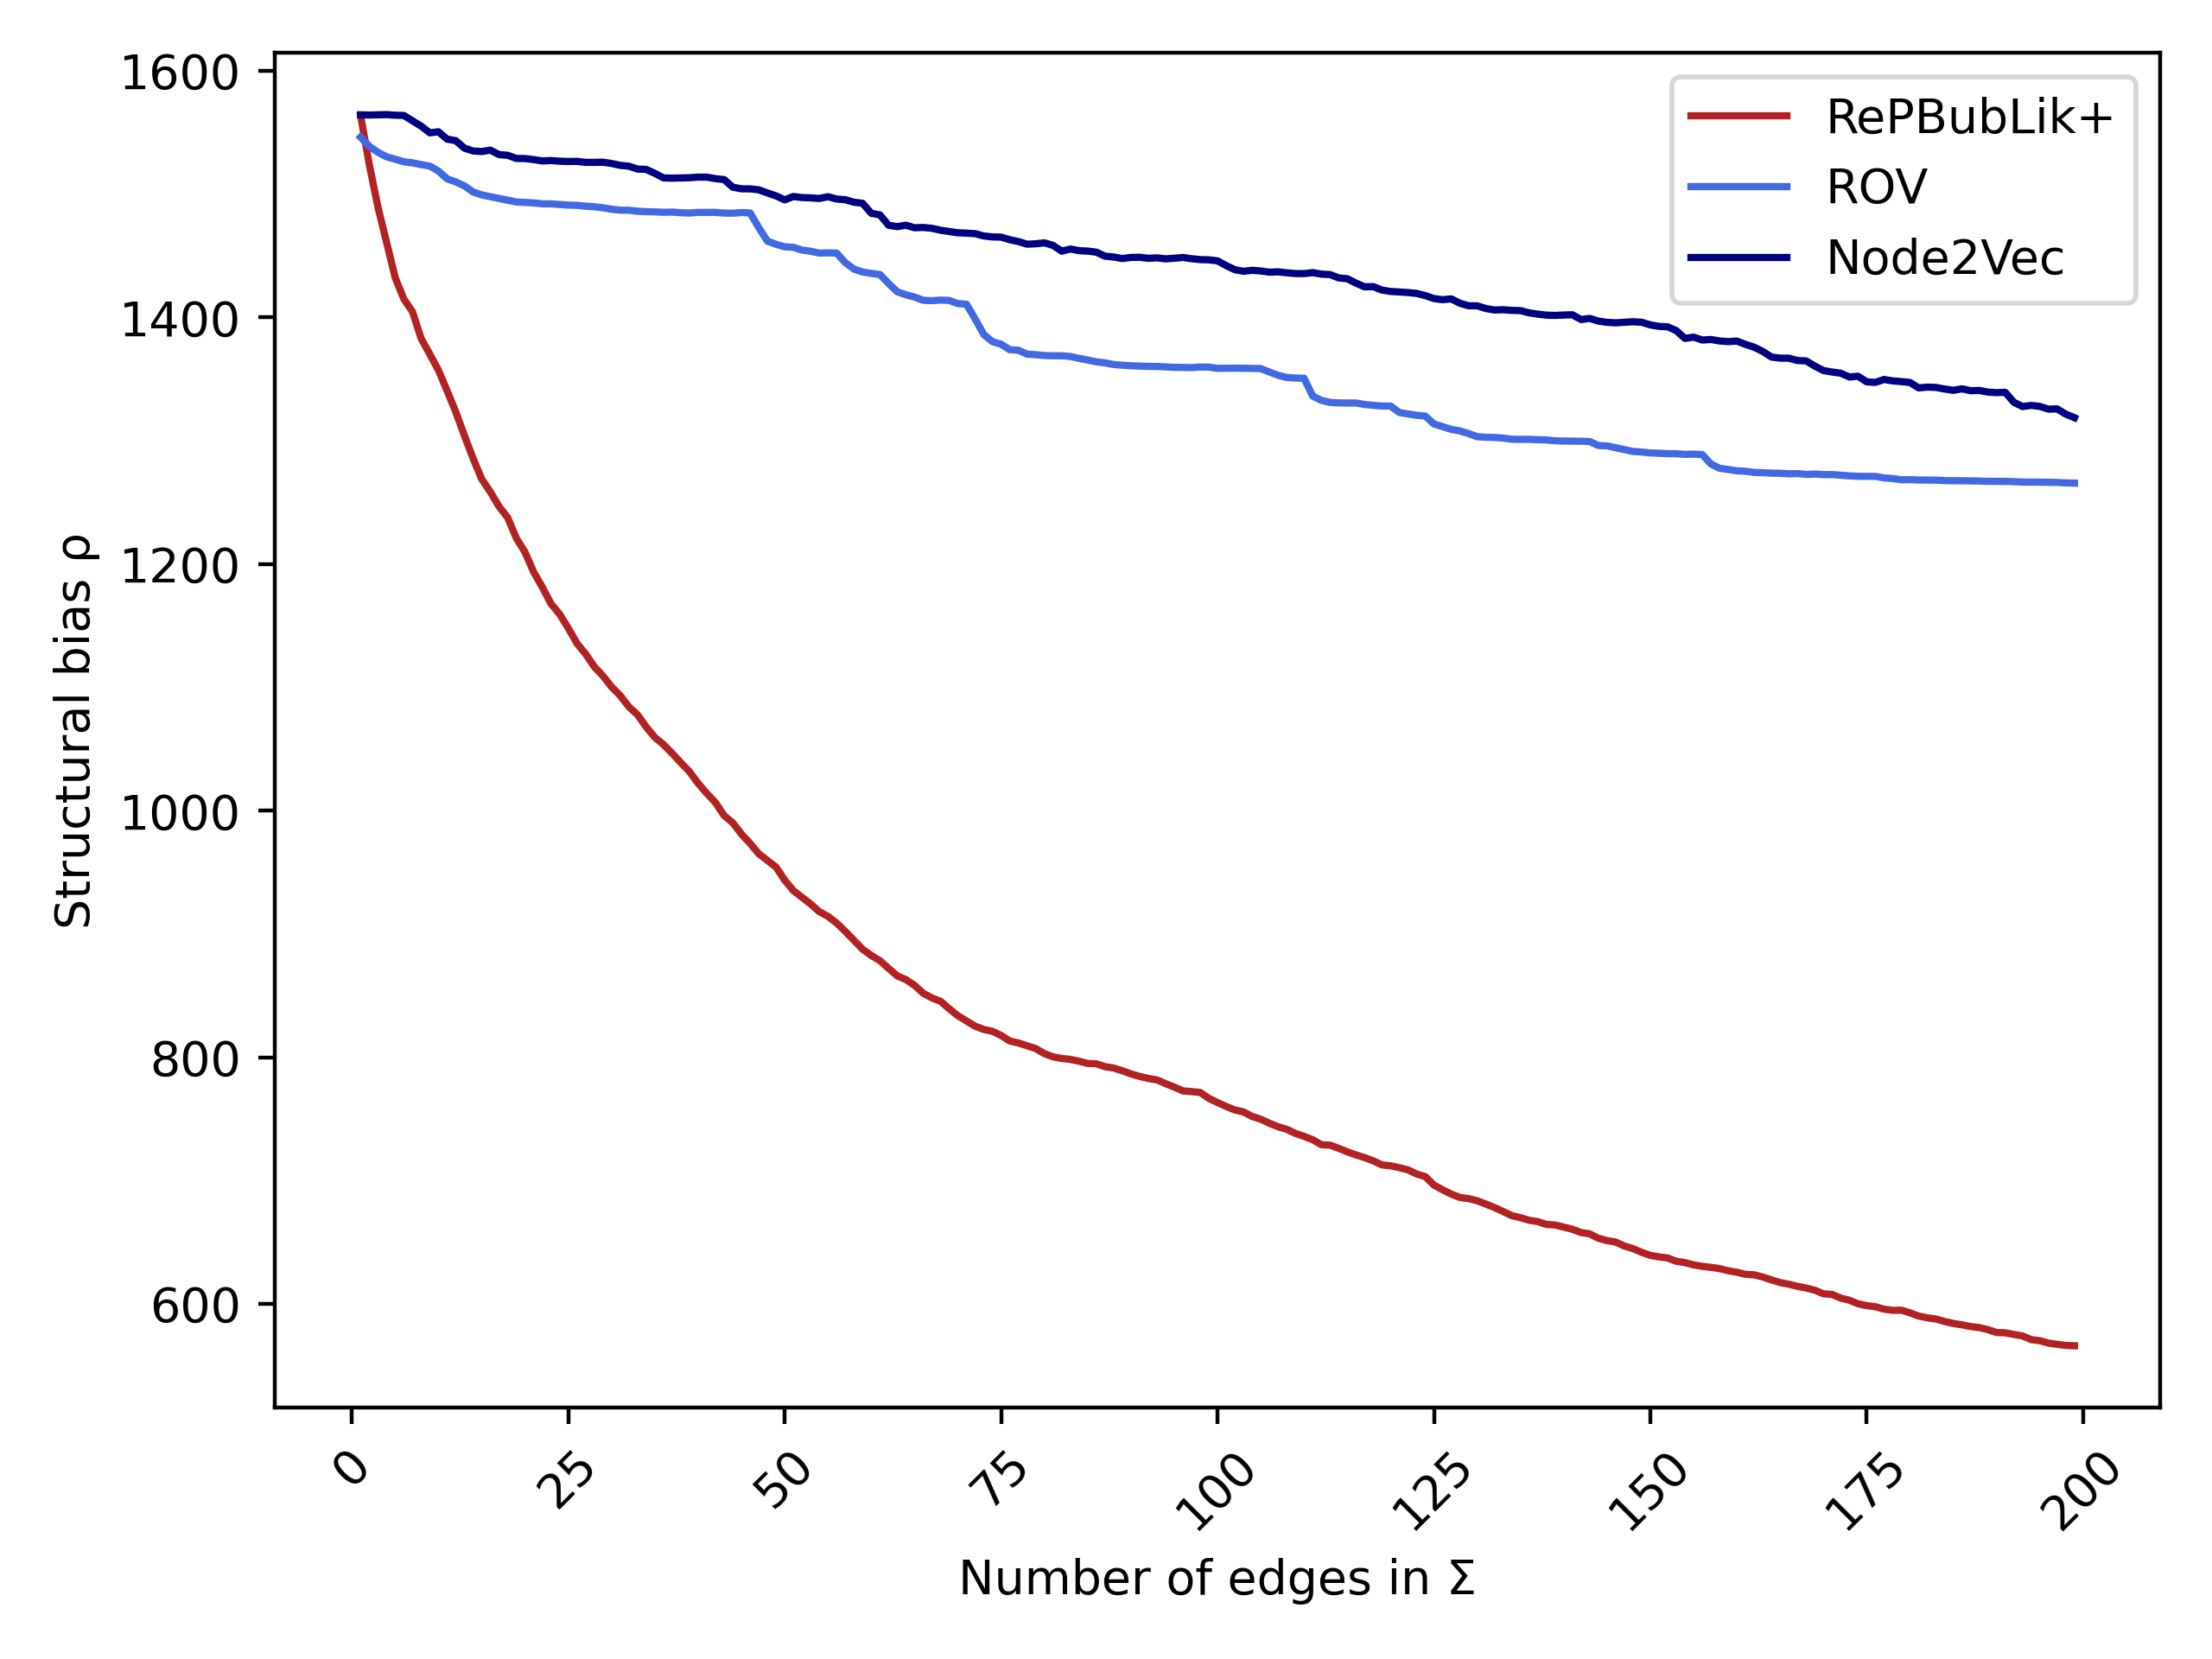
\includegraphics[width=\columnwidth]{5/math_ast_bias_5.png}
    \caption{\emph{MaA}s plot}\label{fig:maas_b_5}
\end{subfigure}
\hspace{0.1\columnwidth}
\begin{subfigure}[b]{0.4\textwidth}
    \centering
    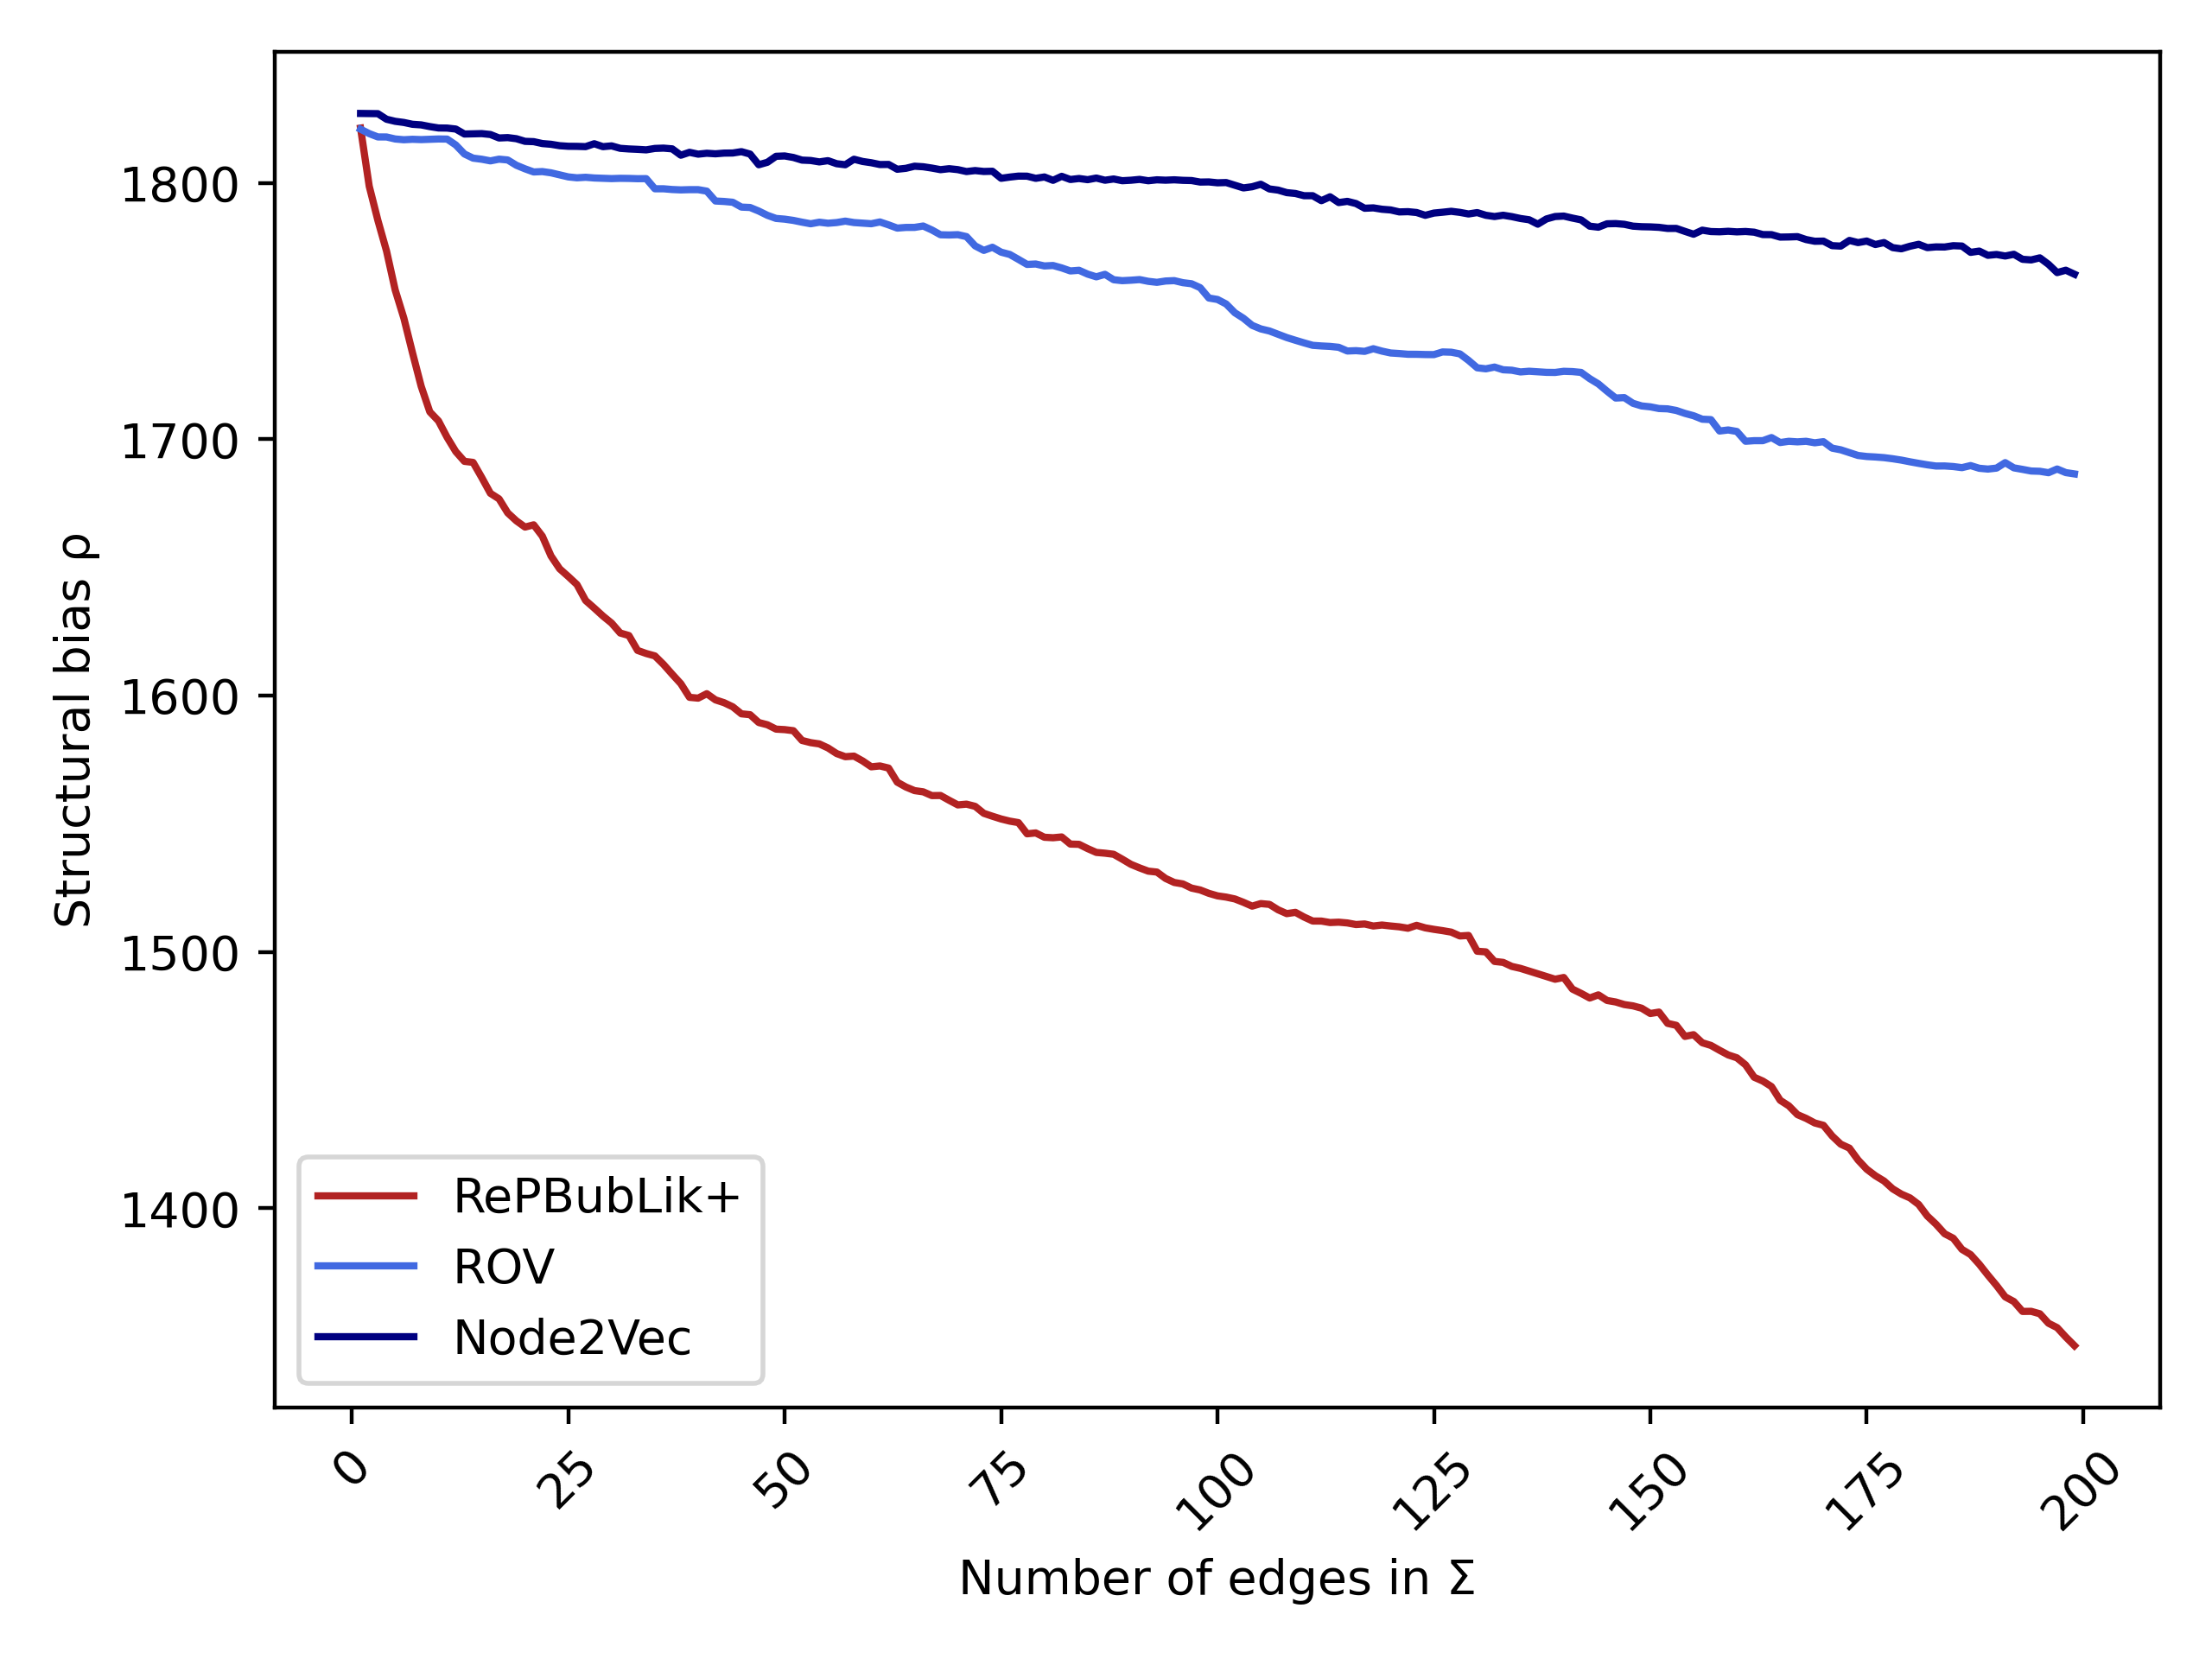
\includegraphics[width=\columnwidth]{5/polblogs_bias_5.png}
    \caption{\emph{PolBlogs} plot}\label{fig:polblogs_b_5}
\end{subfigure}
\caption{Grafici $\rho(G)$ per $t=5$}
\end{figure}
\begin{figure}[!h]
    \centering
\begin{subfigure}[b]{0.4\textwidth}
    \centering
    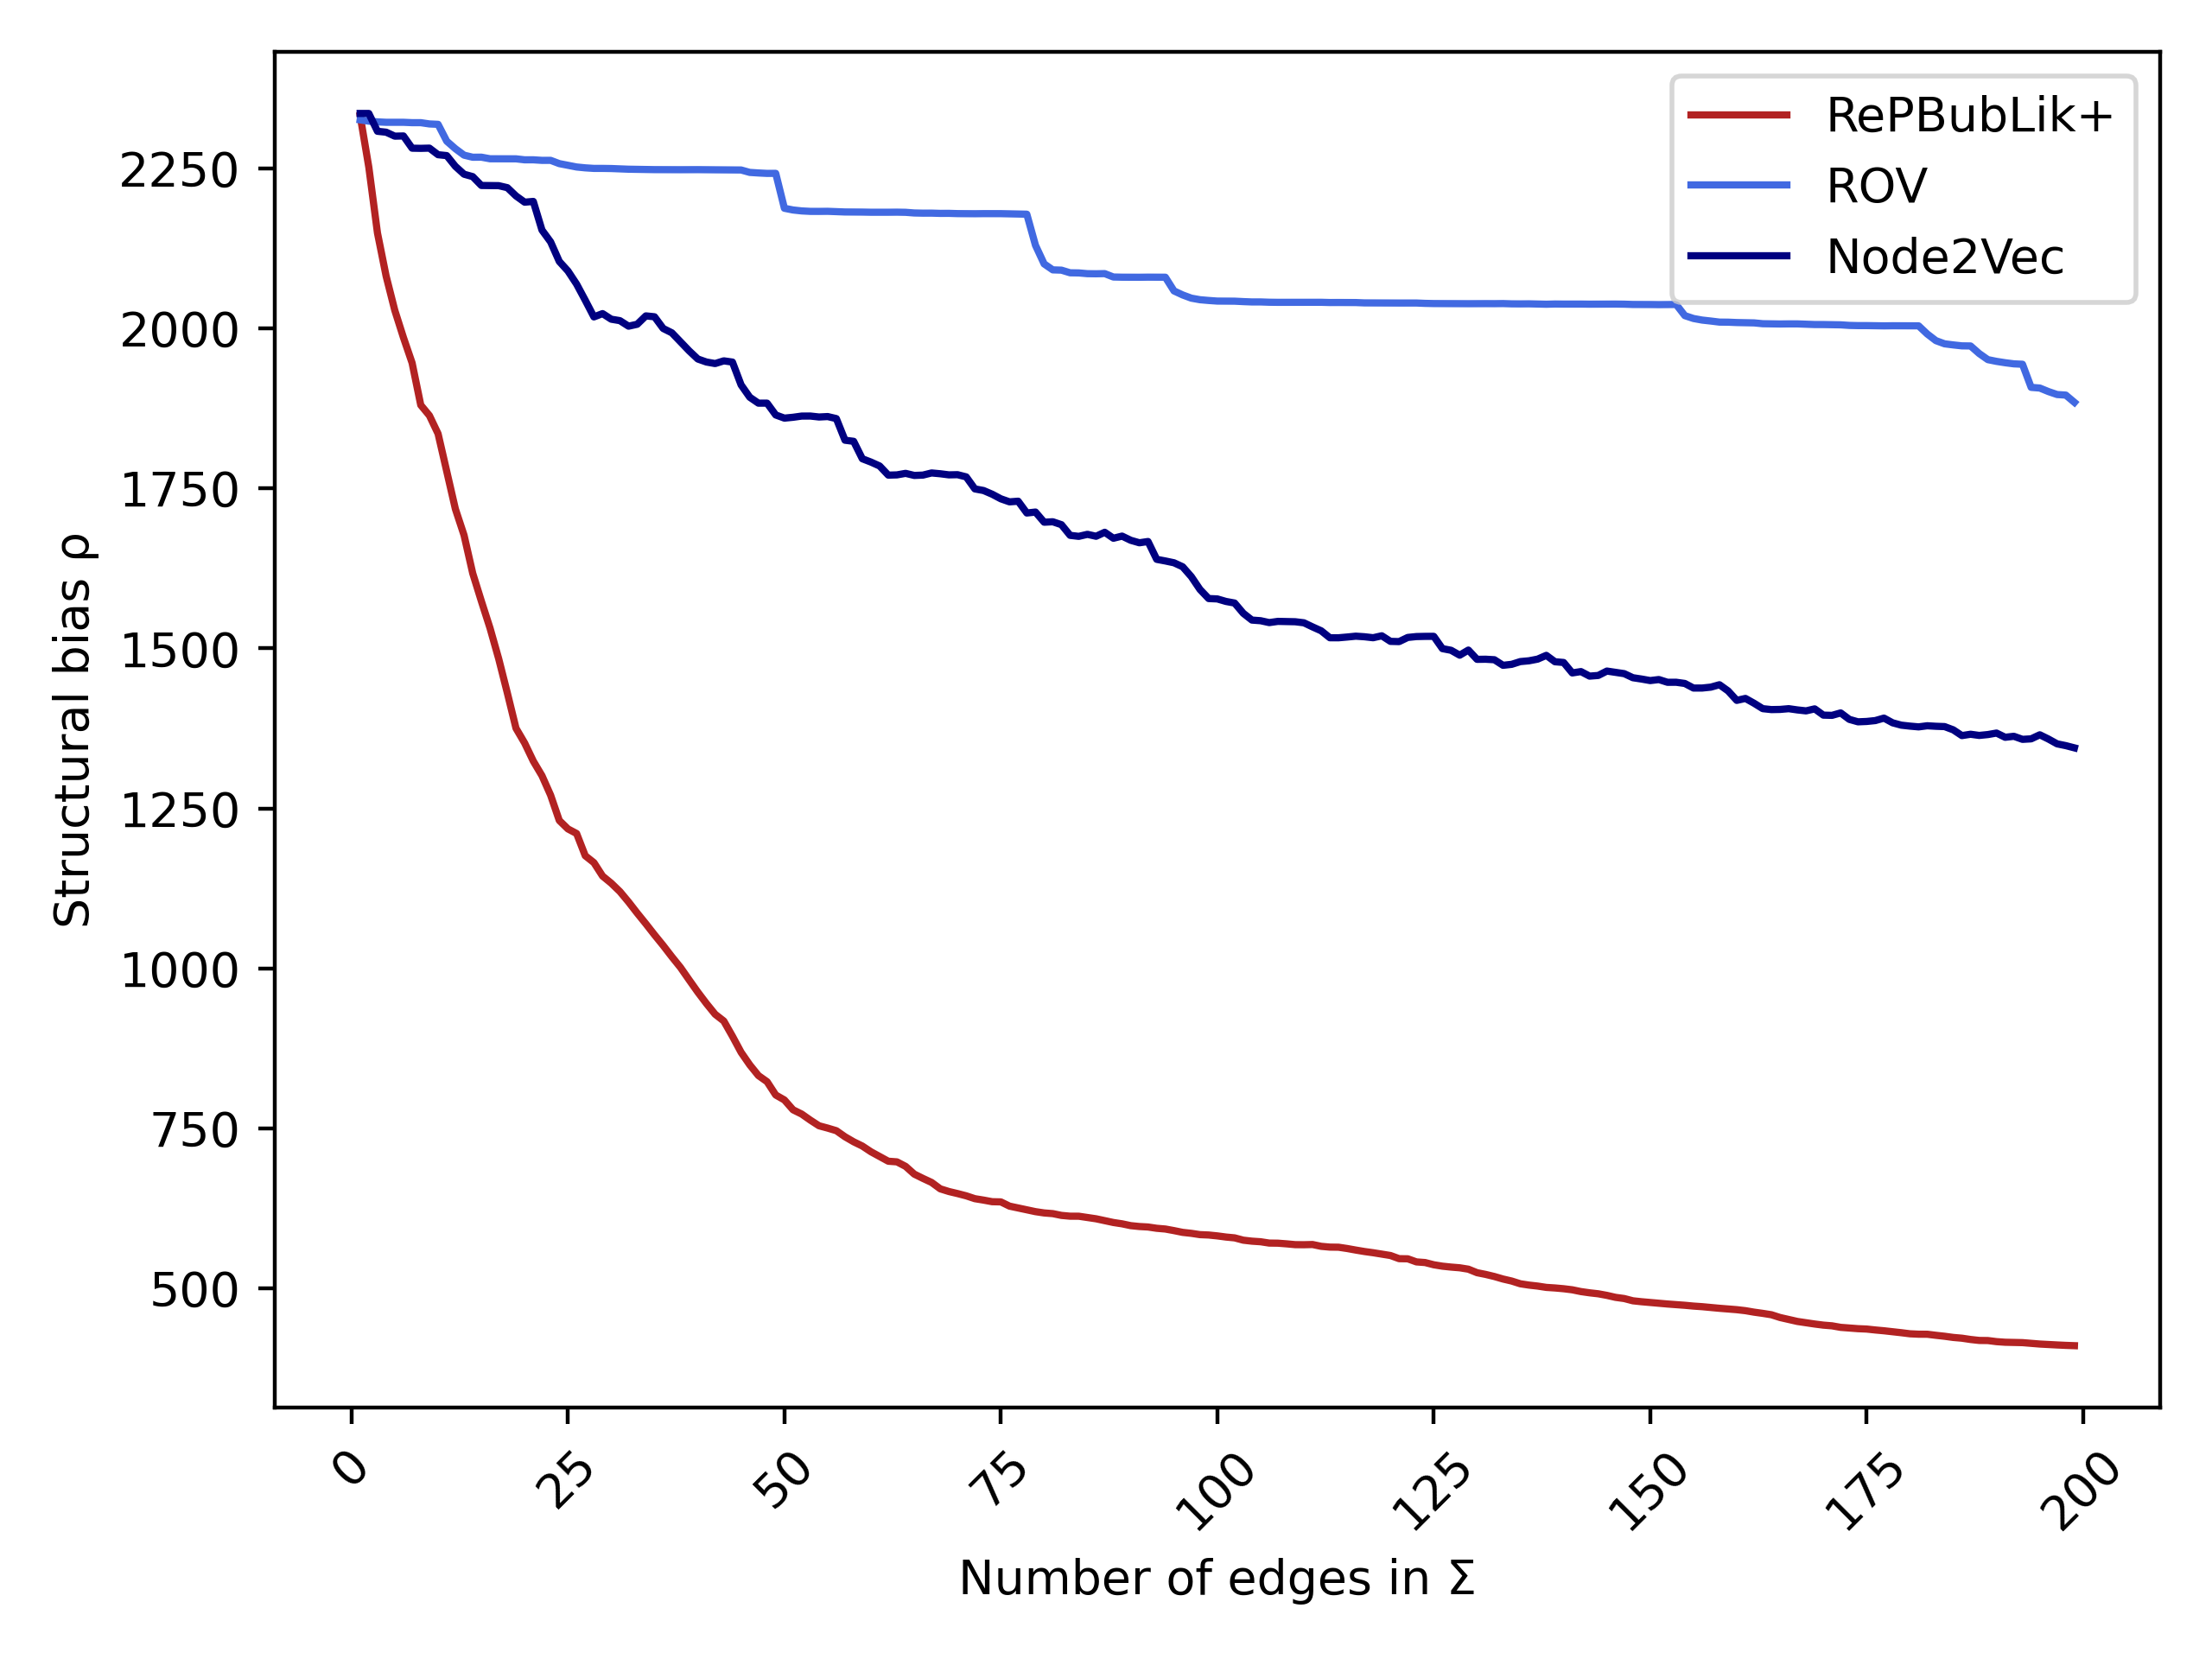
\includegraphics[width=\columnwidth]{10/math_tech_bias_10.png}
    \caption{\emph{MaTe} plot}\label{fig:mate_b_10}
\end{subfigure}
\hspace{0.1\columnwidth}
\begin{subfigure}[b]{0.4\textwidth}
    \centering
    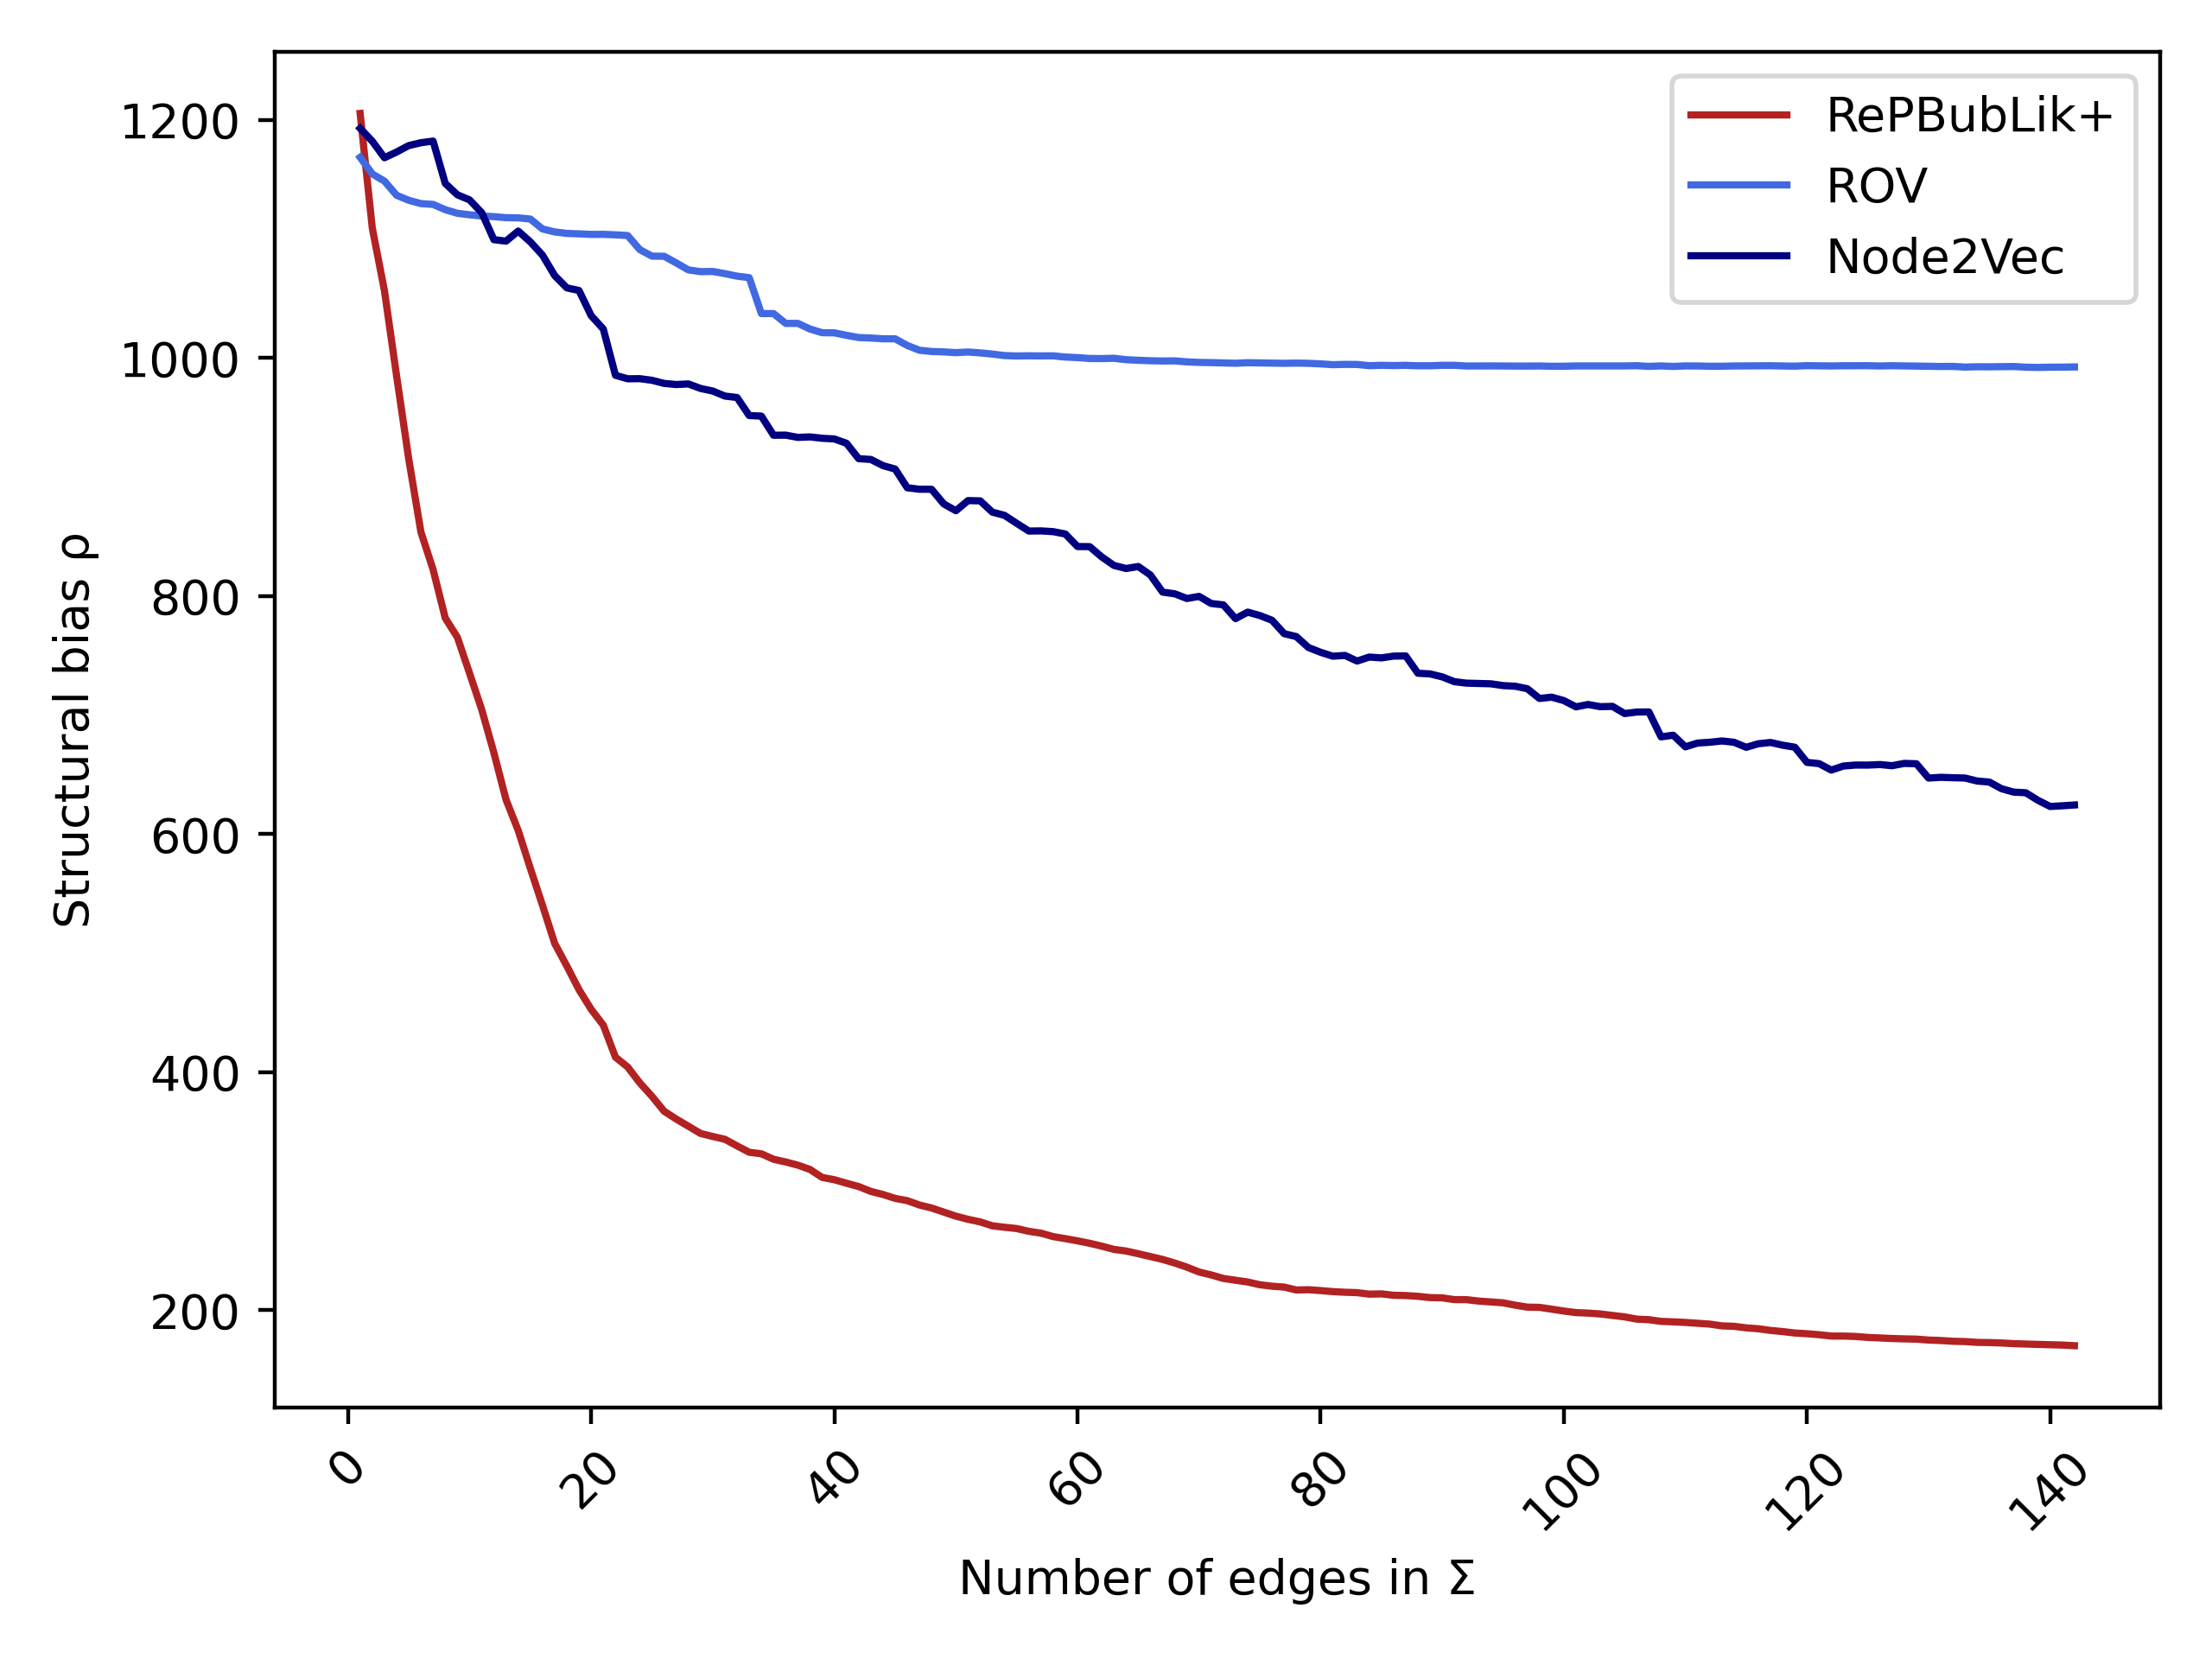
\includegraphics[width=\columnwidth]{10/tech_mil_bias_10.png}
    \caption{\emph{MiHi} plot}\label{fig:mihi_b_10}
\end{subfigure}
\end{figure}
\begin{figure}
    \ContinuedFloat
    \centering
\begin{subfigure}[b]{0.4\textwidth}
    \centering
    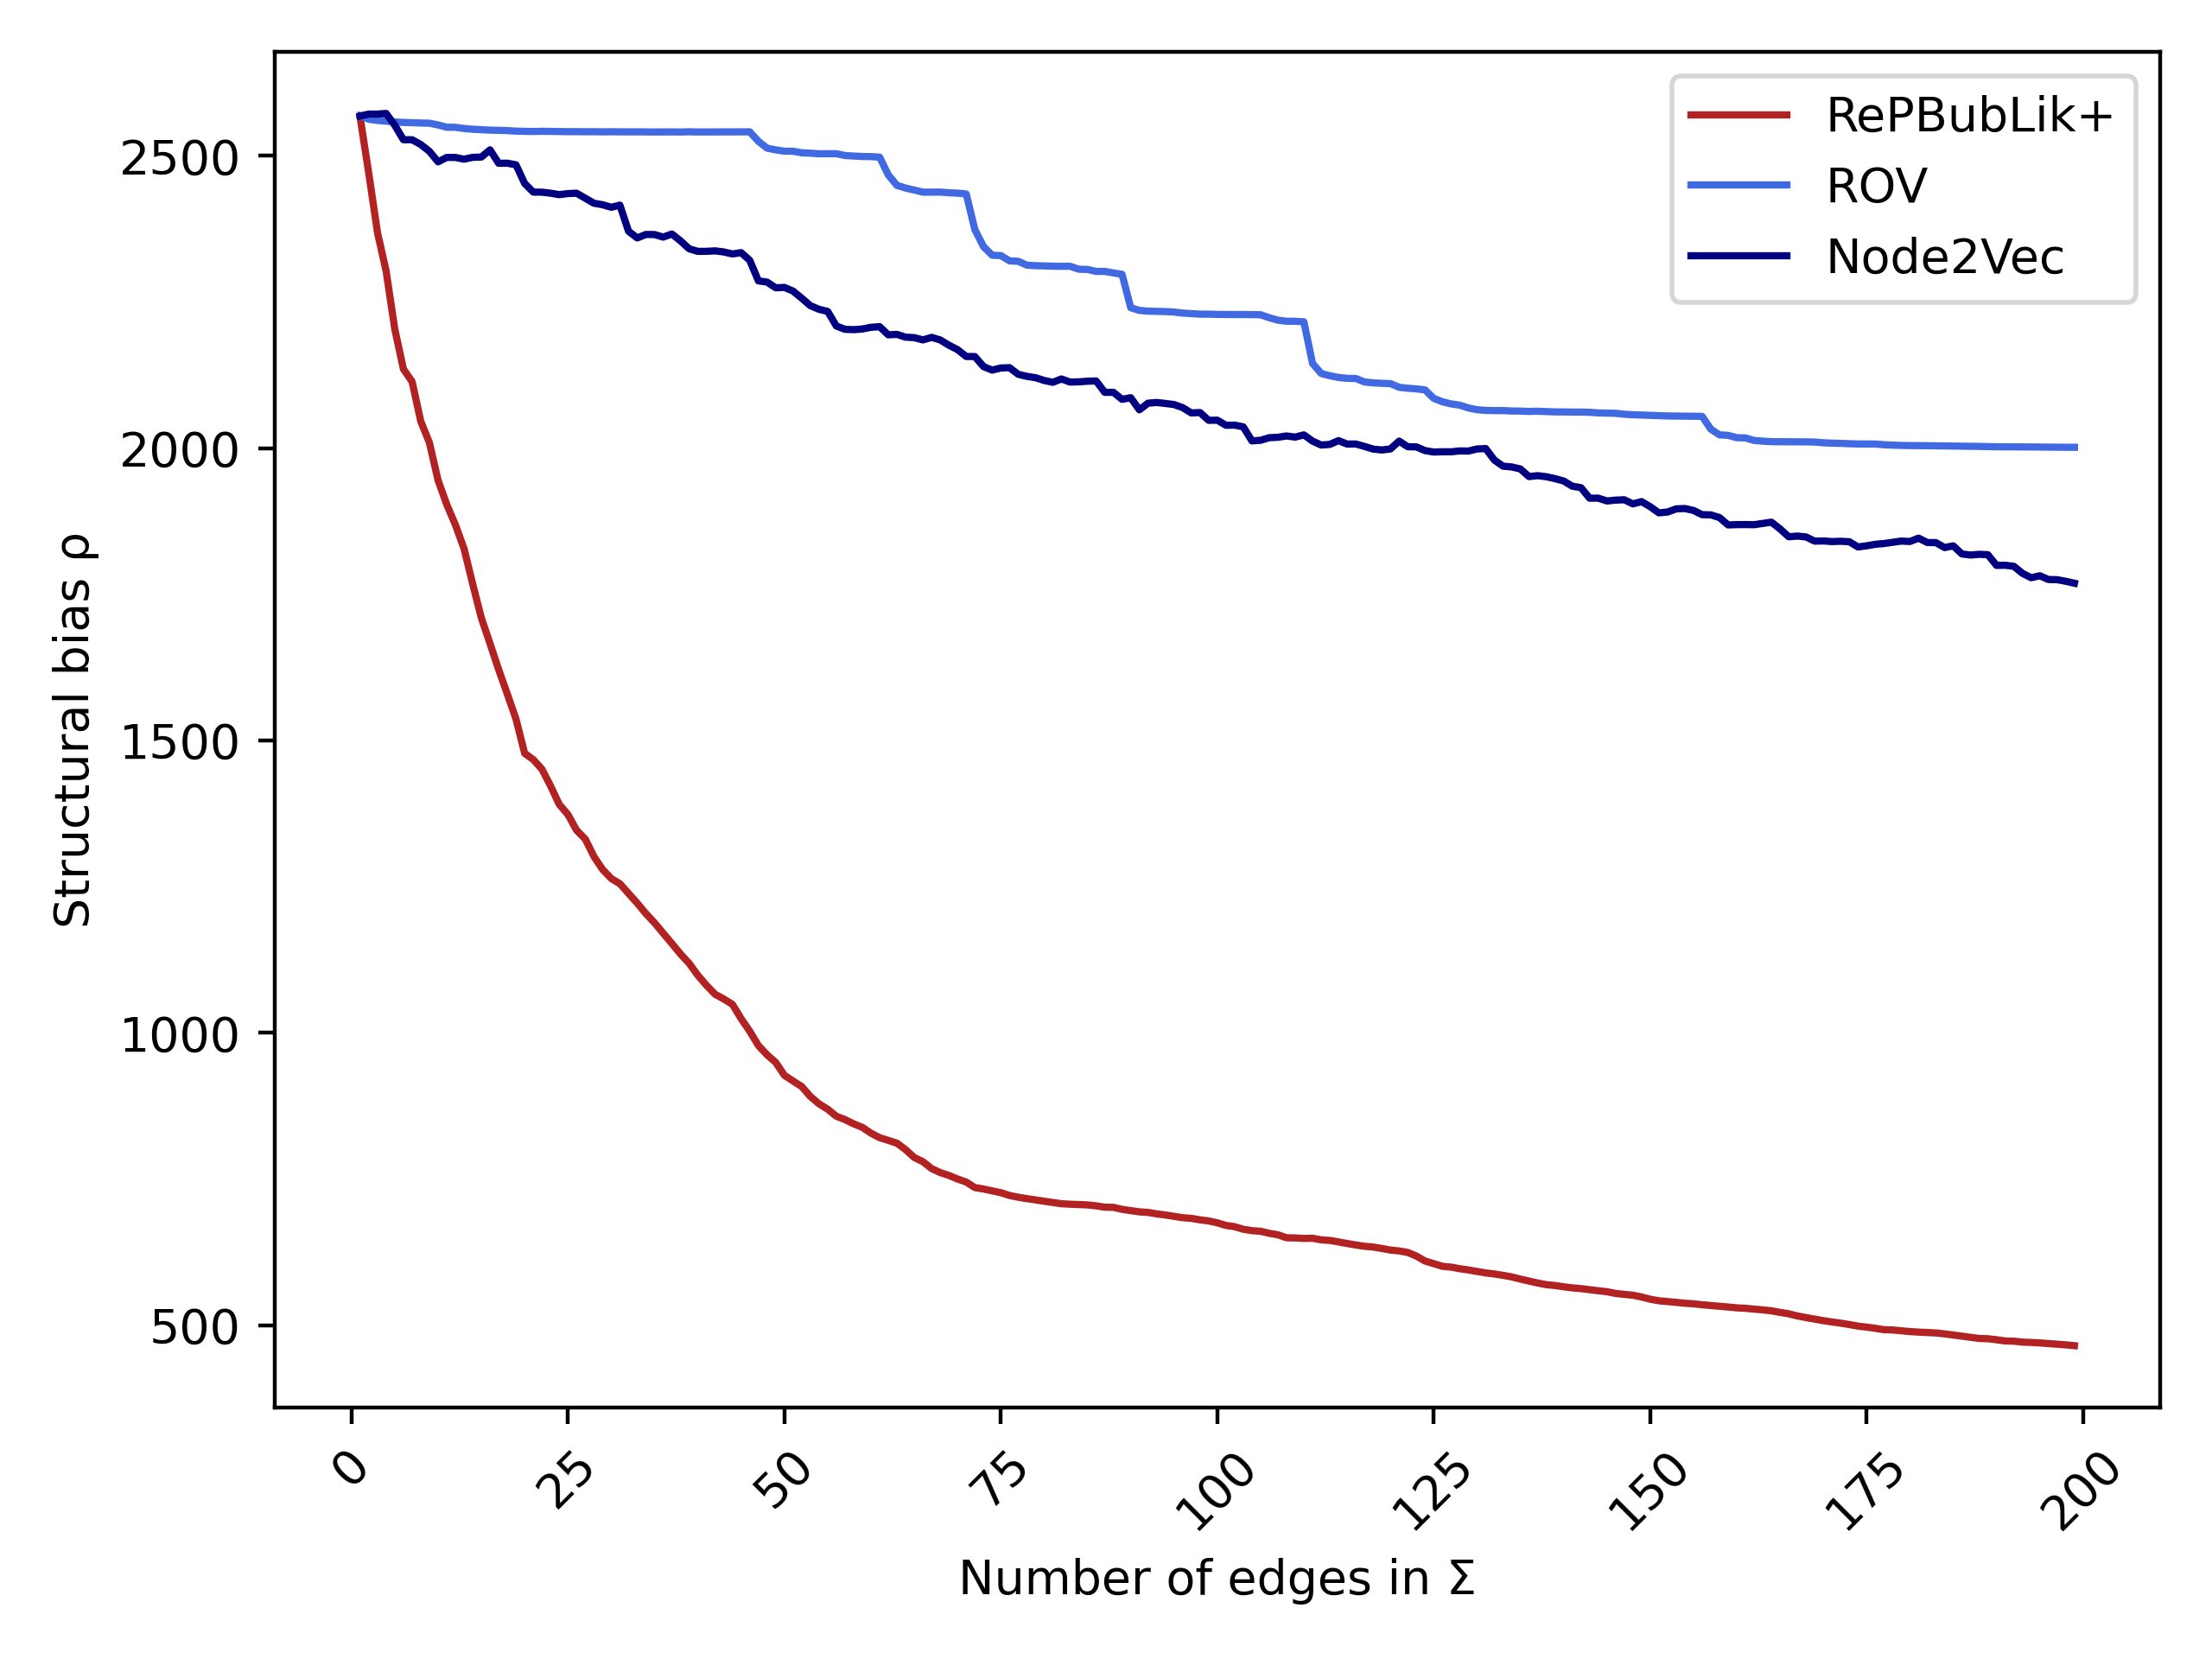
\includegraphics[width=\columnwidth]{10/math_ast_bias_10.png}
    \caption{\emph{MaA}s plot}\label{fig:maas_b_10}
\end{subfigure}
\hspace{0.1\columnwidth}
\begin{subfigure}[b]{0.4\textwidth}
    \centering
    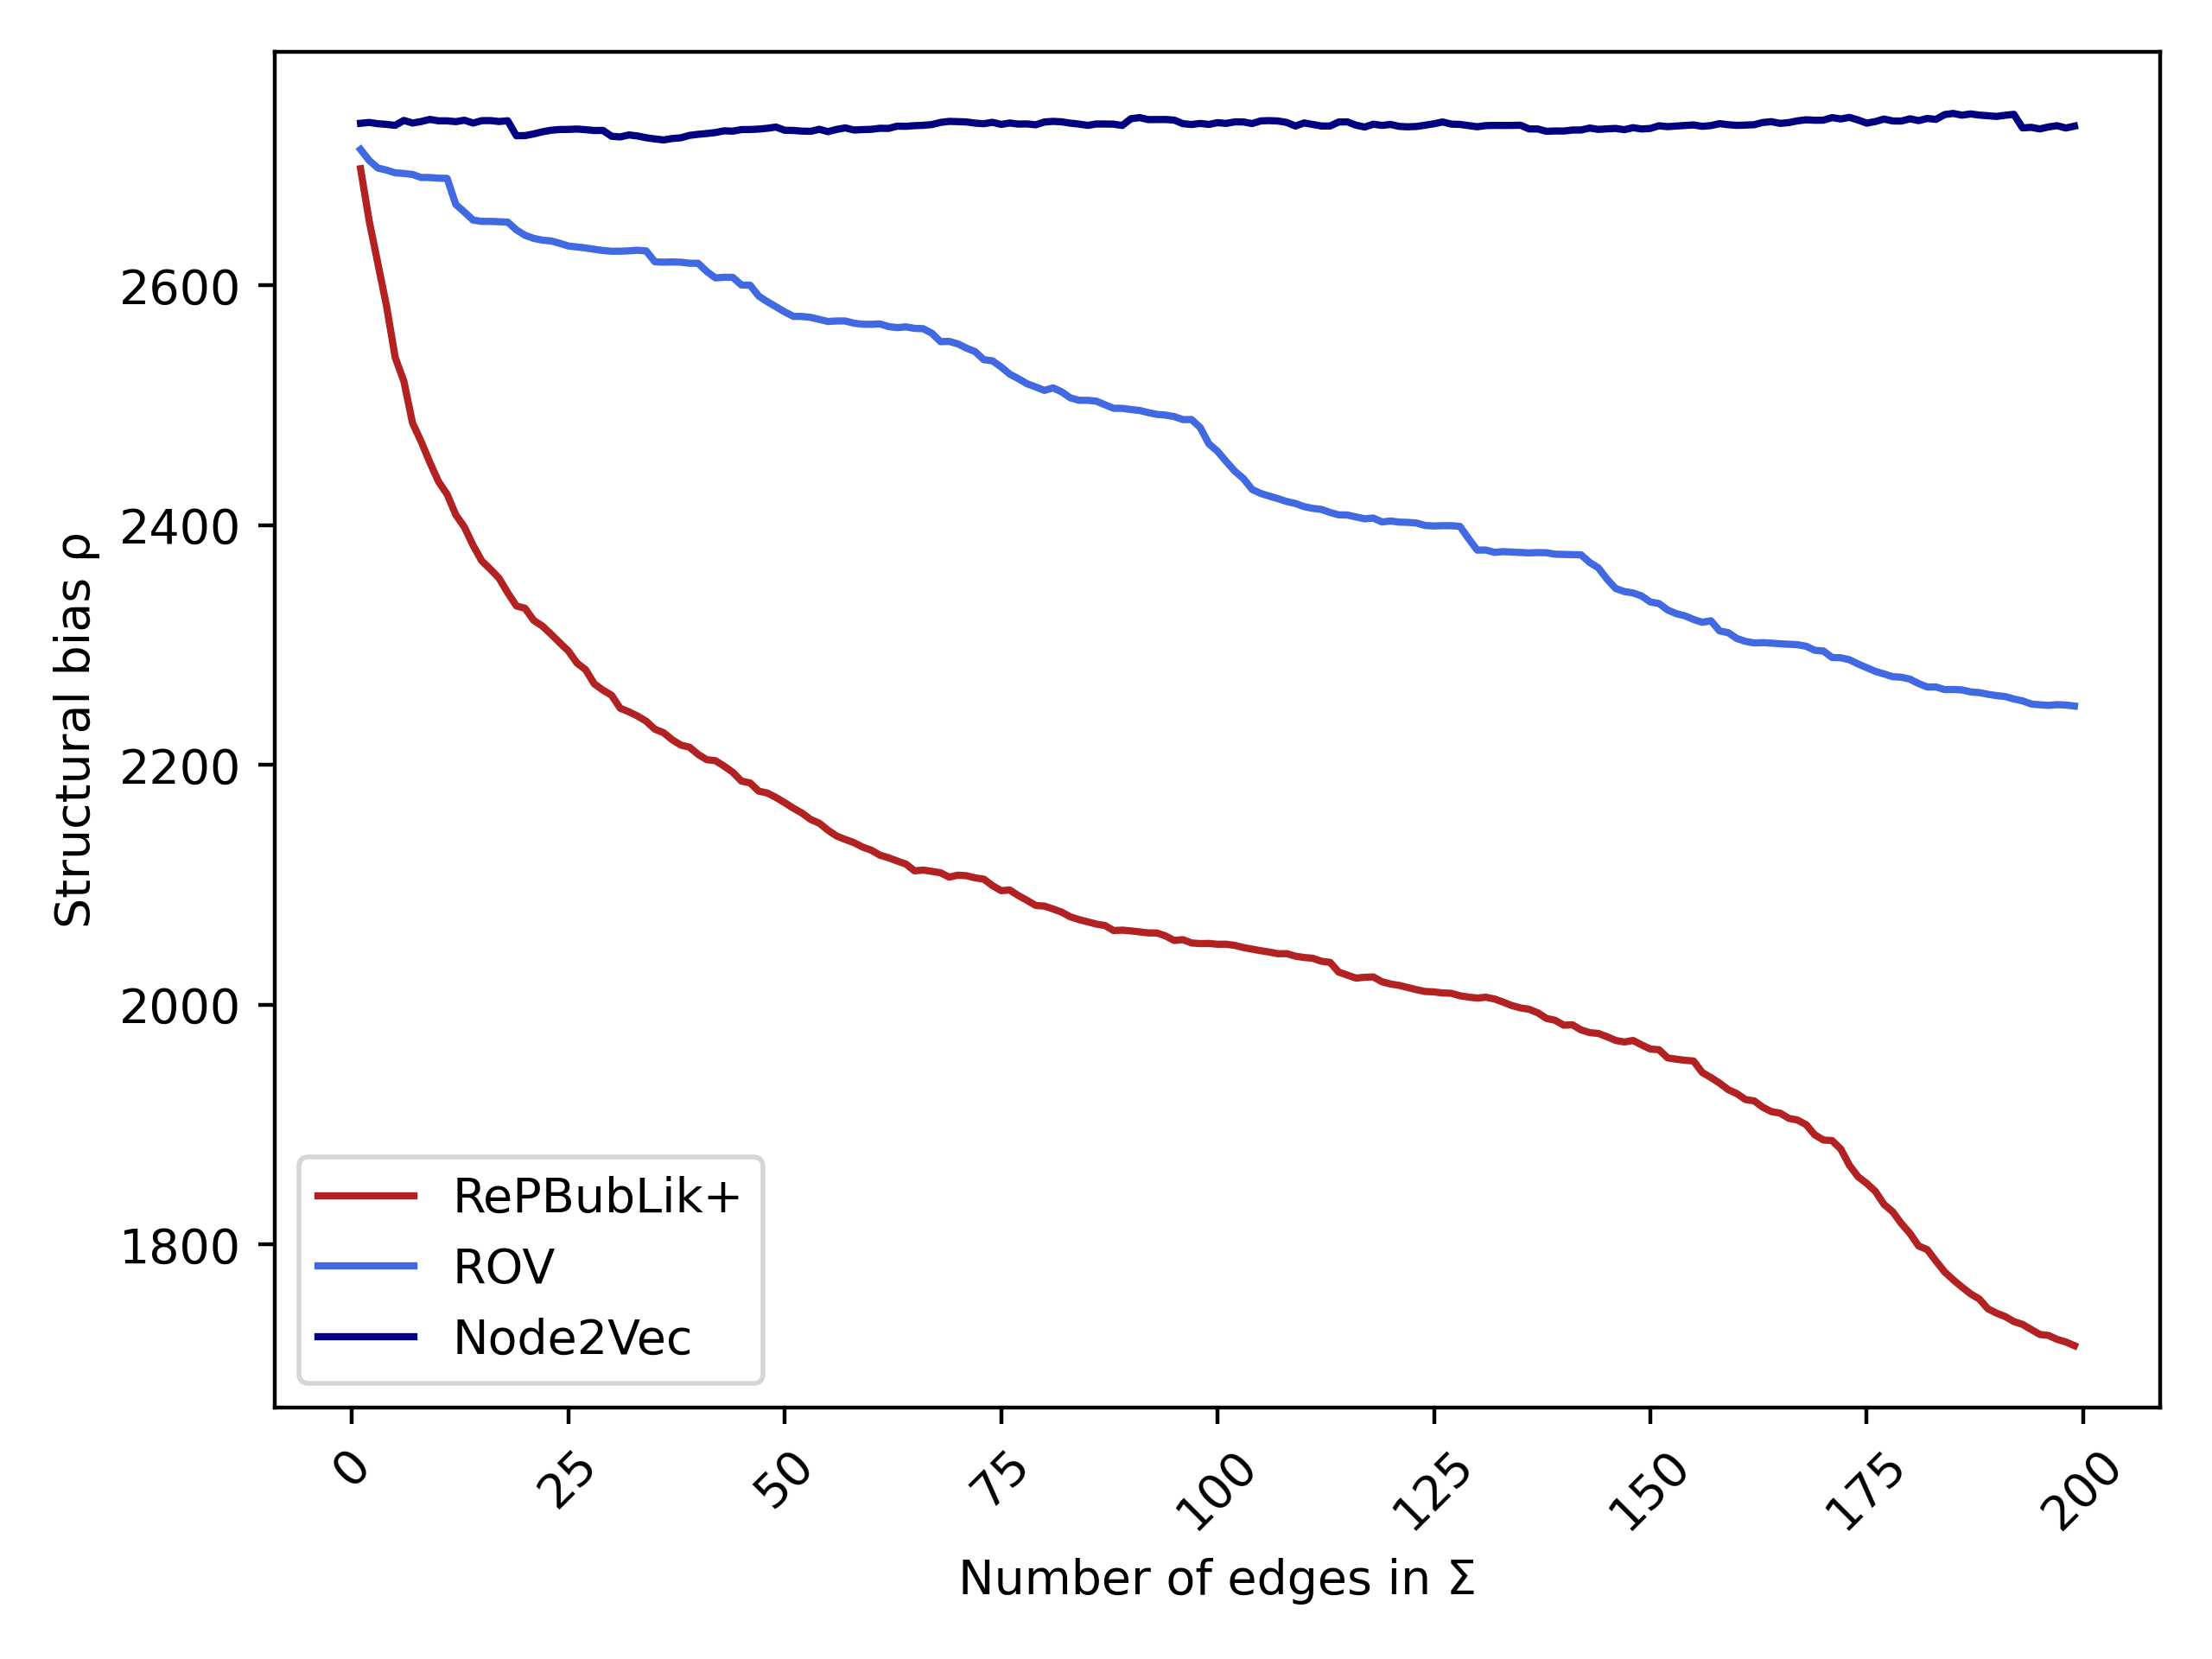
\includegraphics[width=\columnwidth]{10/polblogs_bias_10.png}
    \caption{\emph{PolBlogs} plot}\label{fig:polblogs_b_10}
\end{subfigure}
\caption{Grafici $\rho(G)$ per $t=10$}
\end{figure}
\newpage
\begin{figure}[!h]
    \centering
\begin{subfigure}[b]{0.4\textwidth}
    \centering
    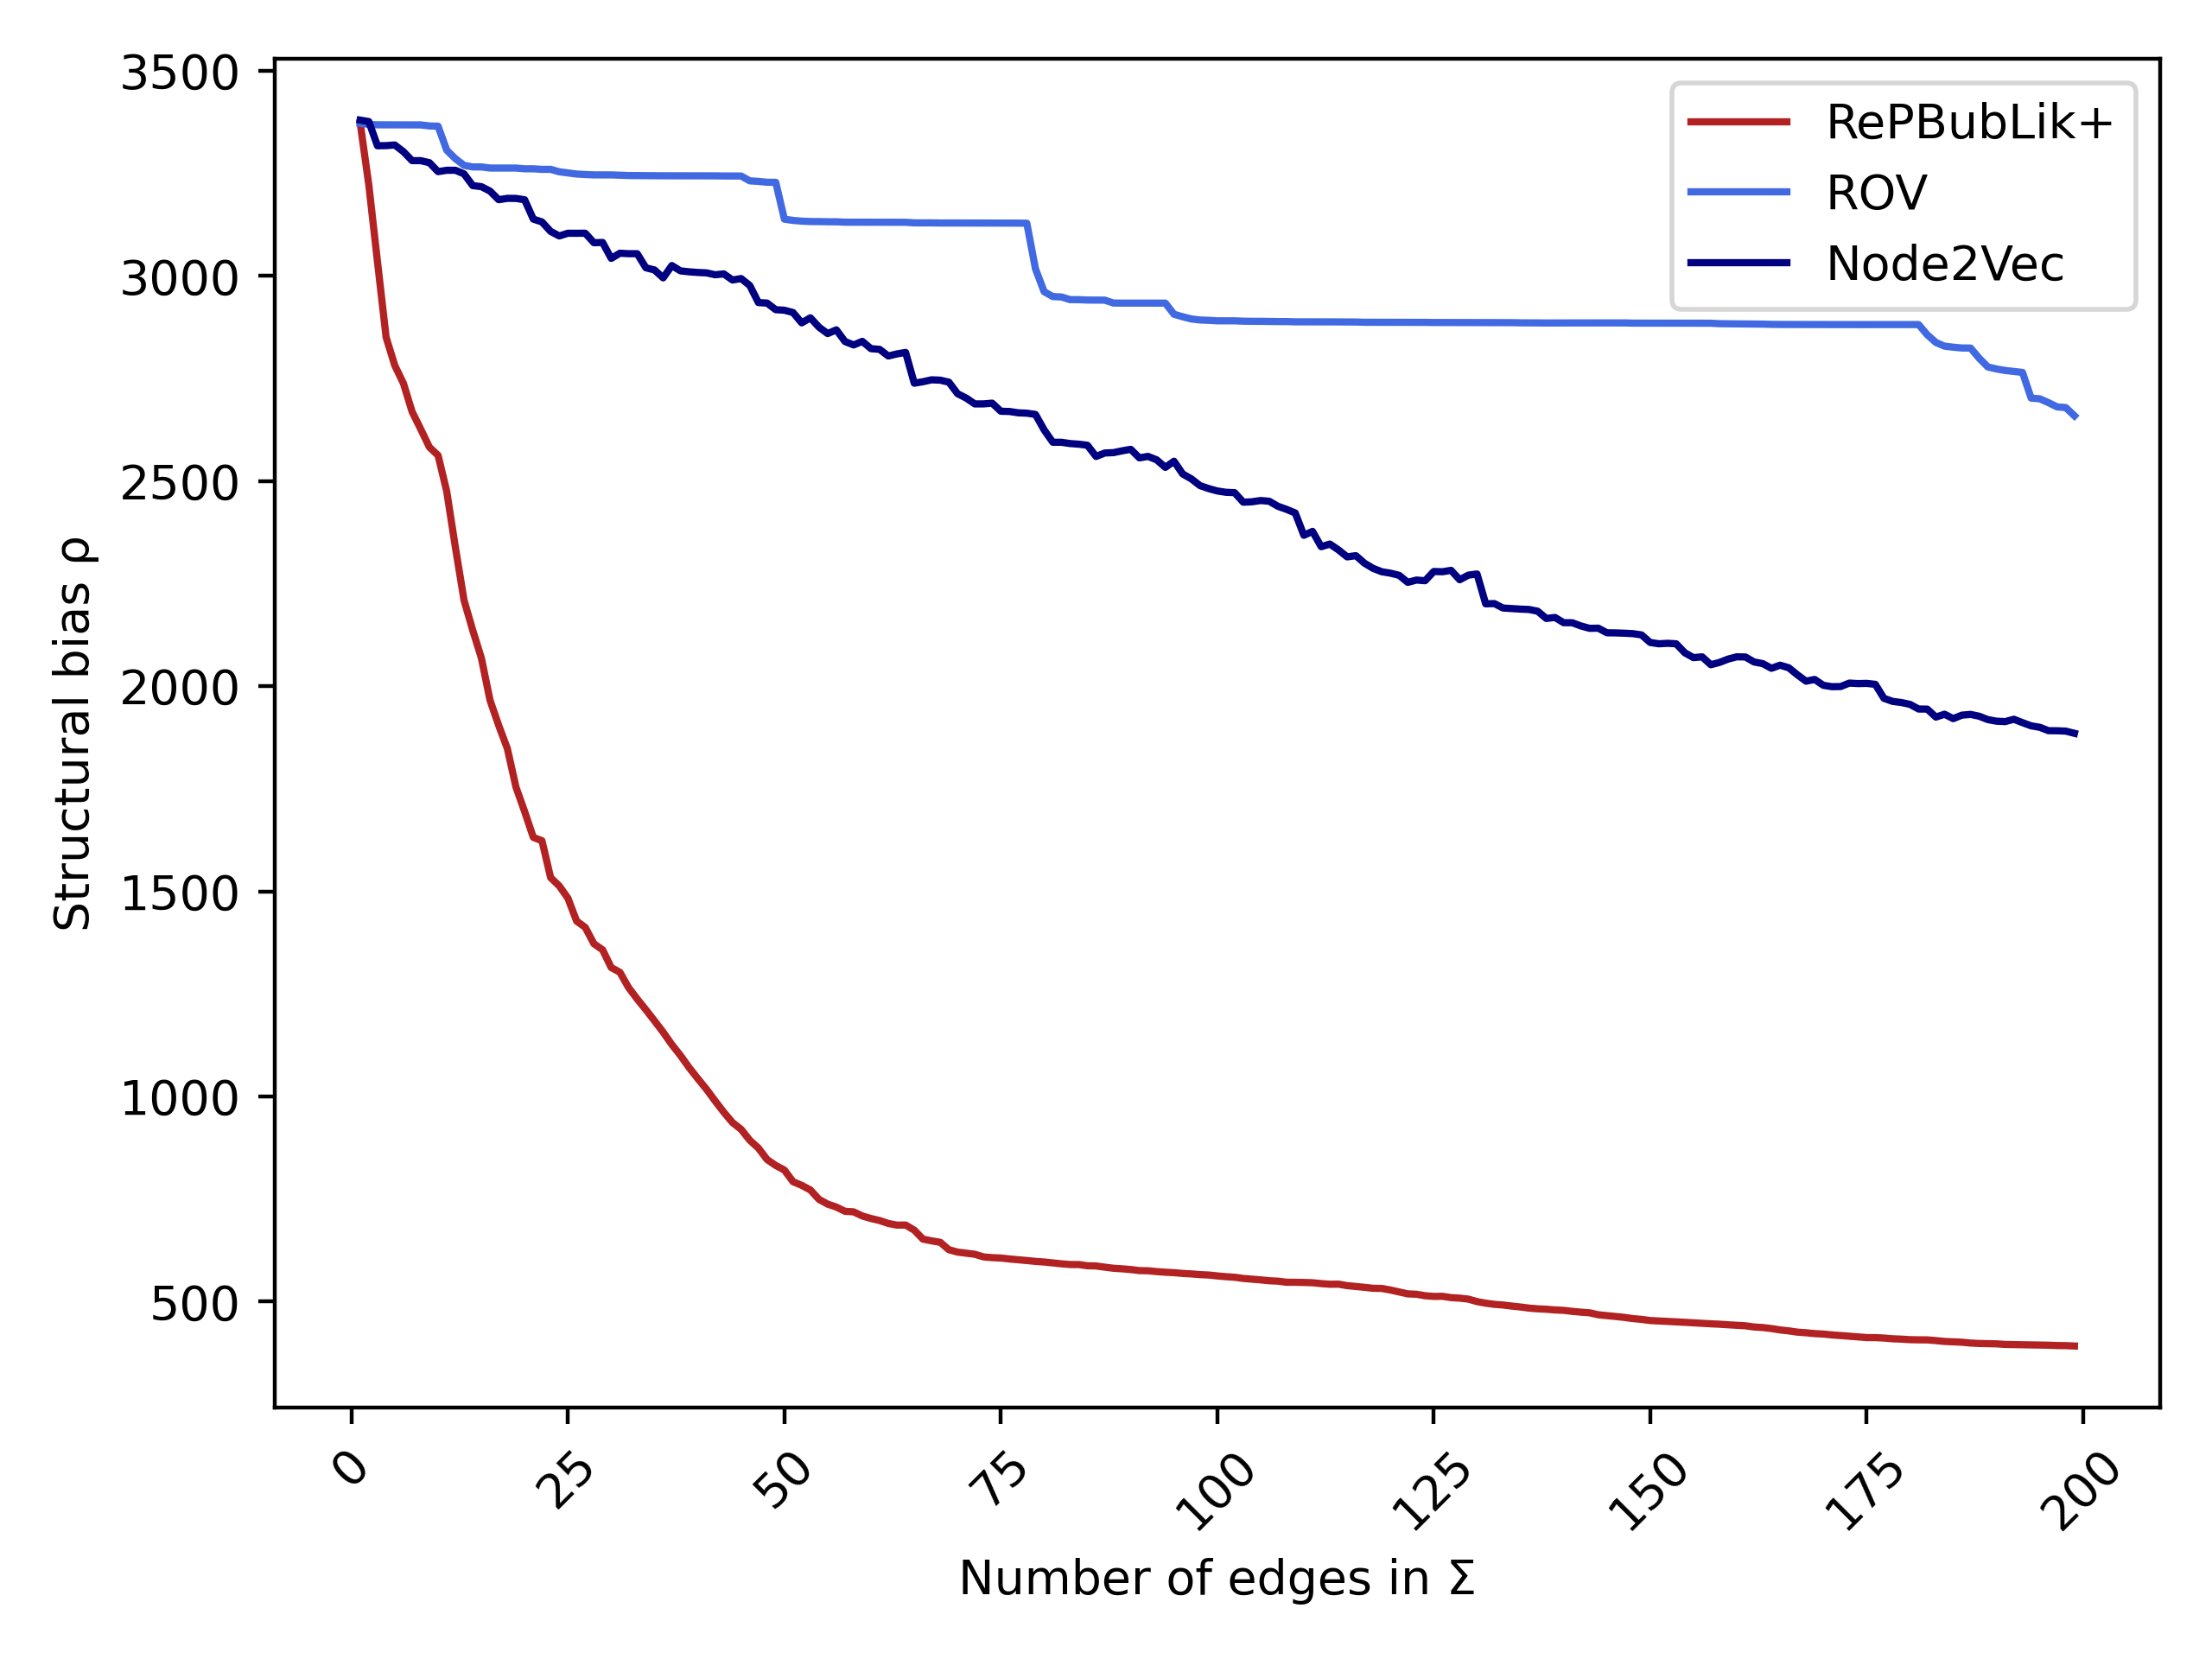
\includegraphics[width=\columnwidth]{15/math_tech_bias_15.png}
    \caption{\emph{MaTe} plot}\label{fig:mate_b_15}
\end{subfigure}
\hspace{0.1\columnwidth}
\begin{subfigure}[b]{0.4\textwidth}
    \centering
    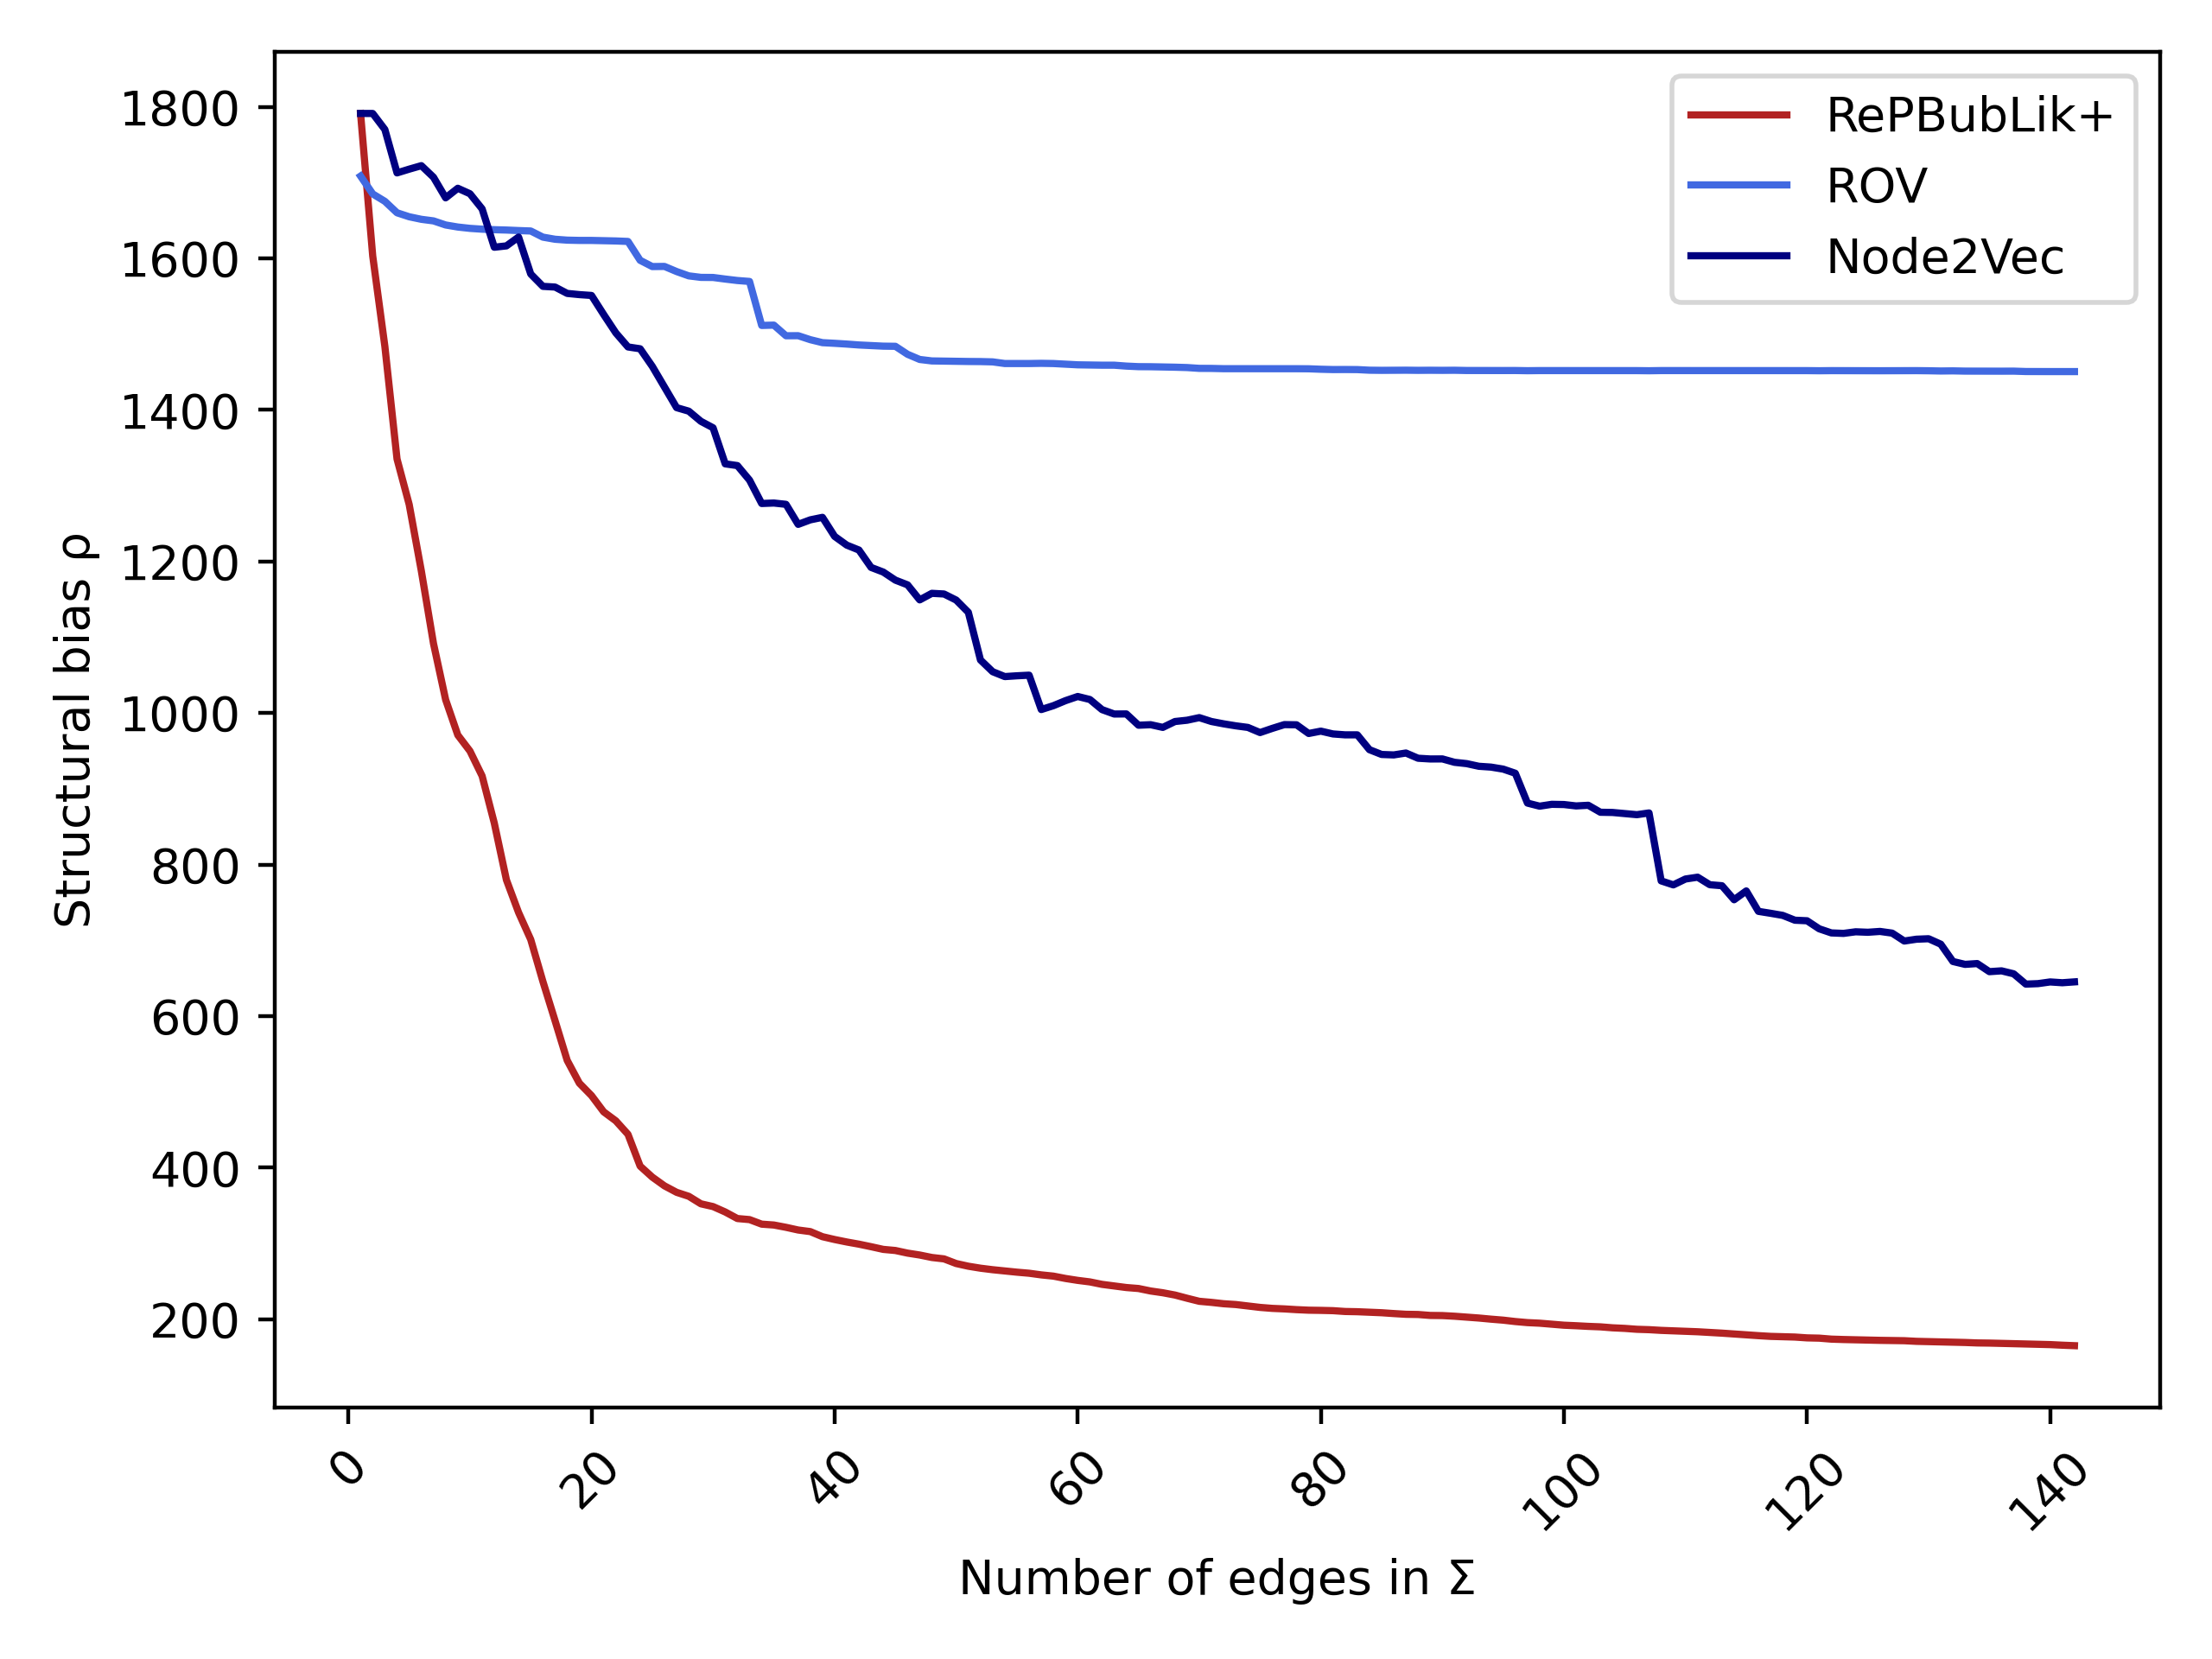
\includegraphics[width=\columnwidth]{15/tech_mil_bias_15.png}
    \caption{\emph{MiHi} plot}\label{fig:mihi_b_15}
\end{subfigure}

\begin{subfigure}[b]{0.4\textwidth}
    \centering
    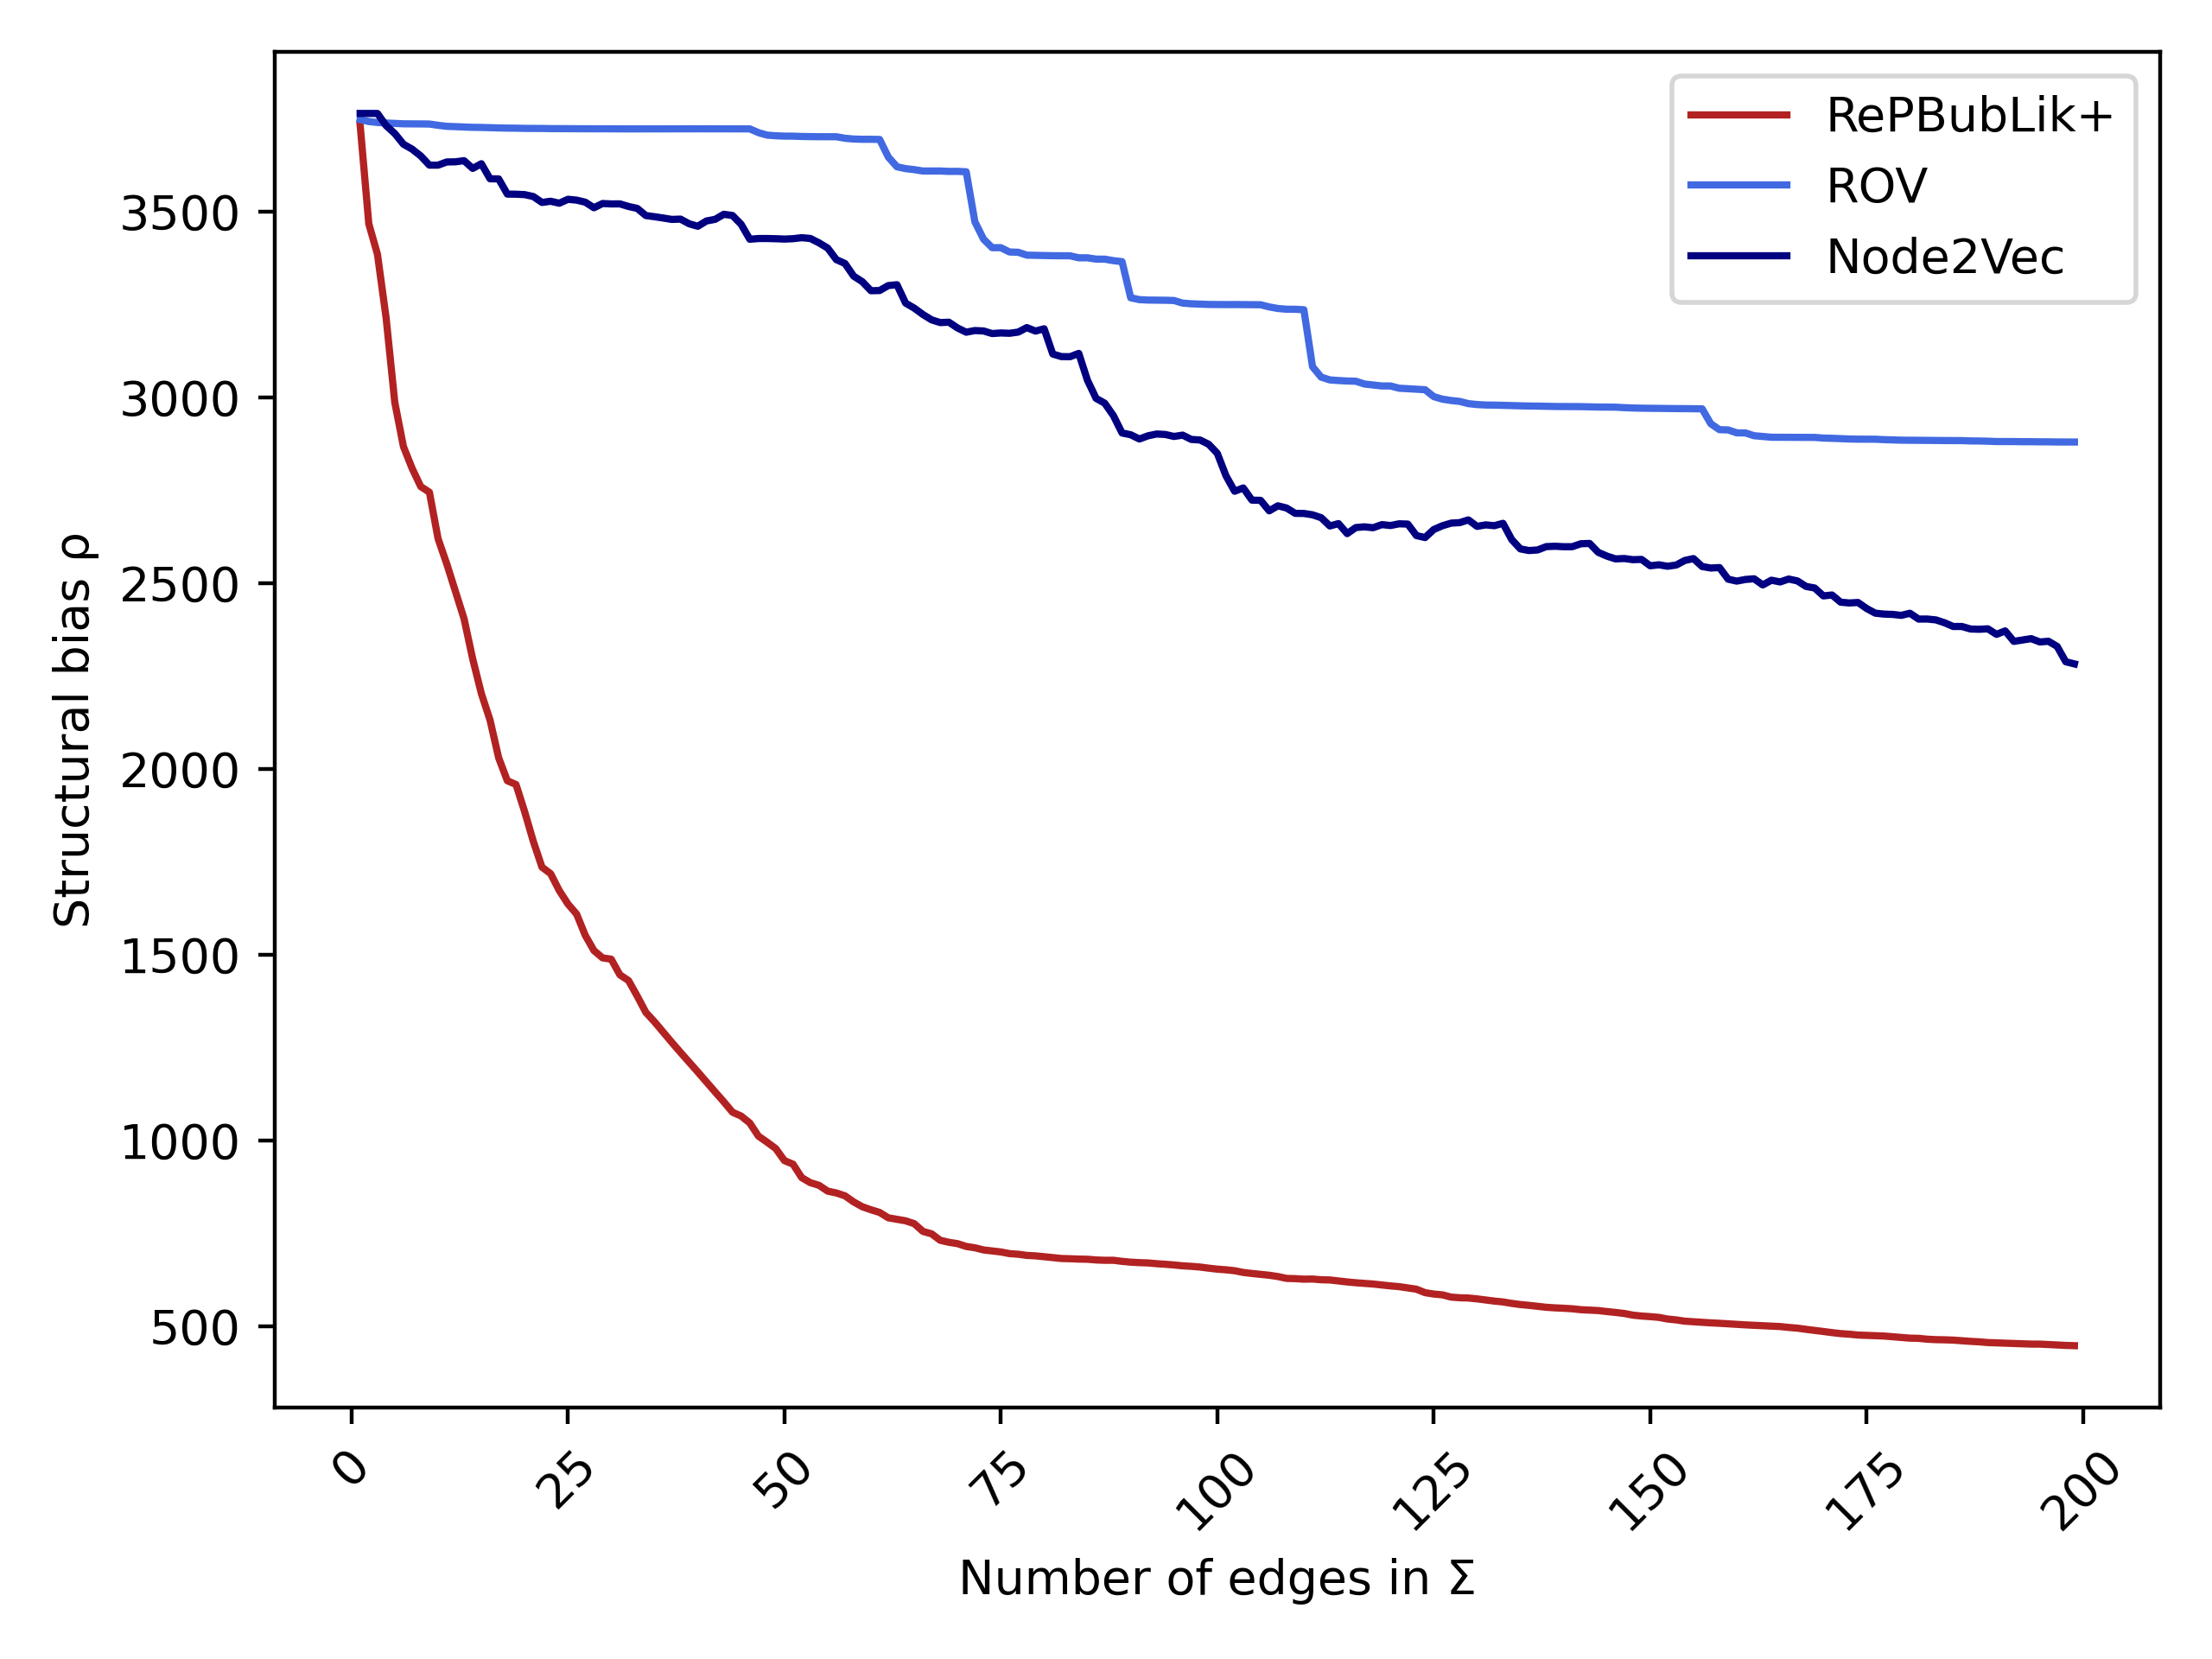
\includegraphics[width=\columnwidth]{15/math_ast_bias_15.png}
    \caption{\emph{MaA}s plot}\label{fig:maas_b_15}
\end{subfigure}
\hspace{0.1\columnwidth}
\begin{subfigure}[b]{0.4\textwidth}
    \centering
    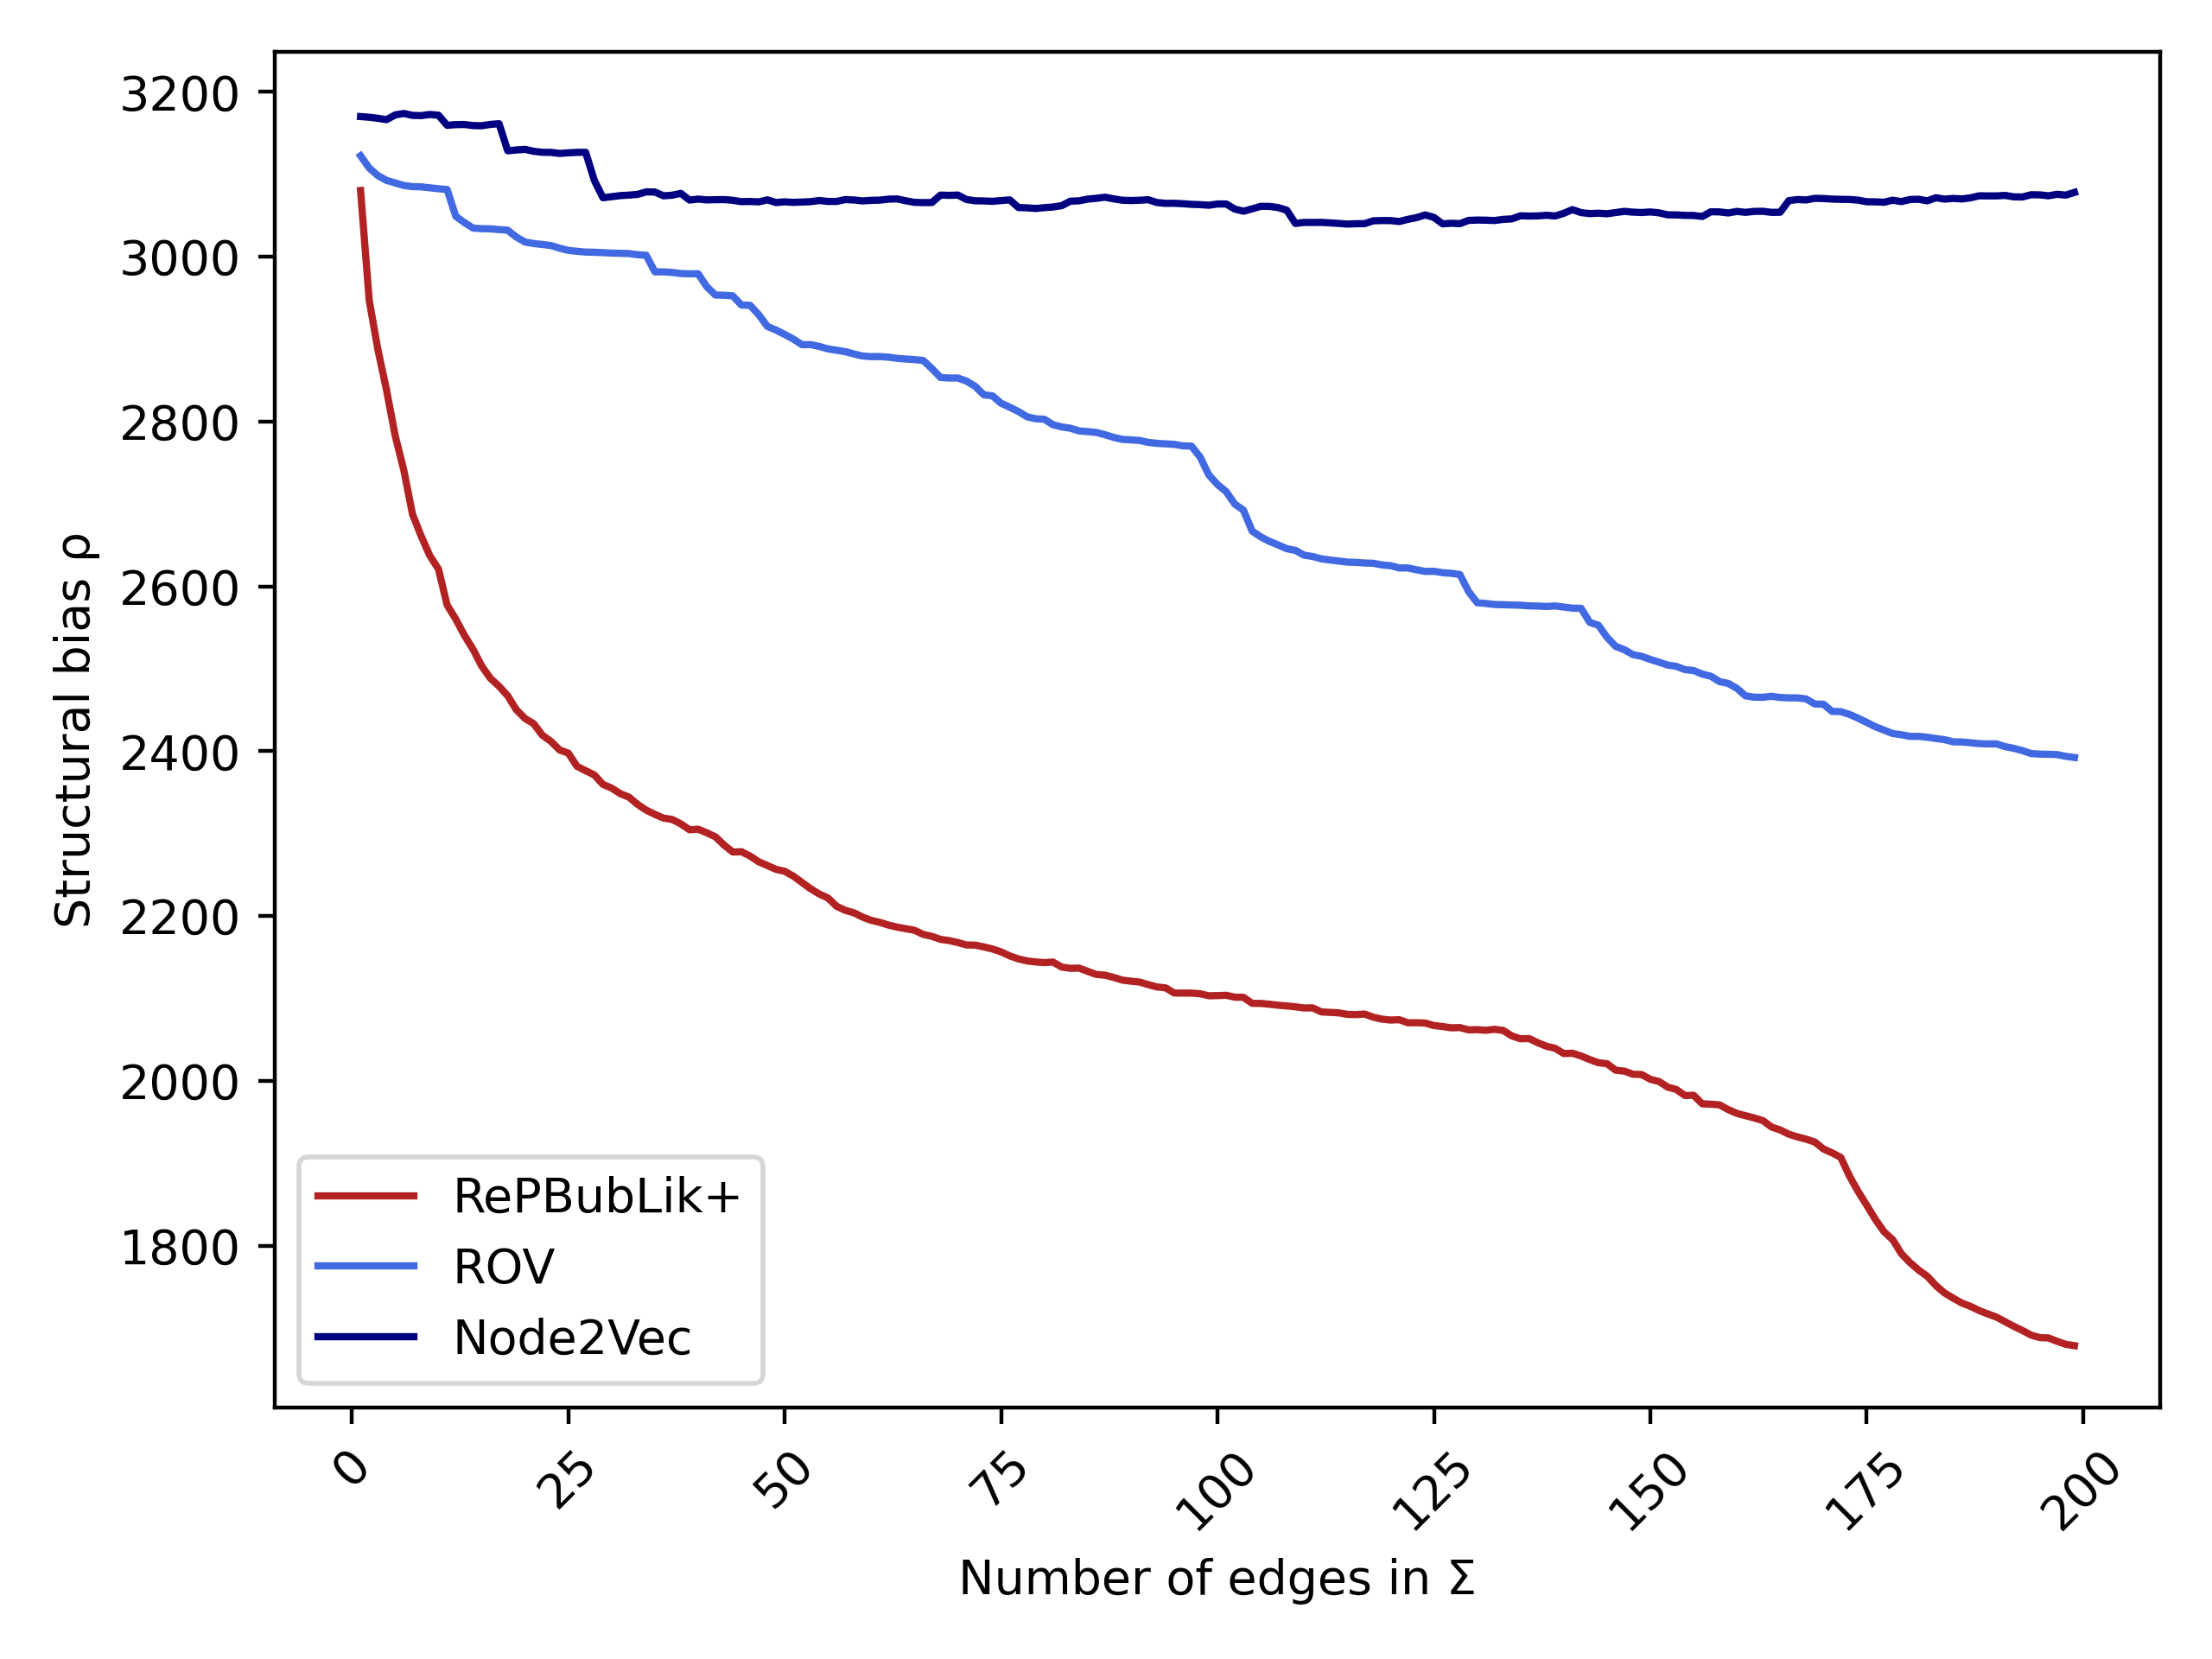
\includegraphics[width=\columnwidth]{15/polblogs_bias_15.png}
    \caption{\emph{PolBlogs} plot}\label{fig:polblogs_b_15}
\end{subfigure}
\caption{Grafici $\rho(G)$ per $t=15$}
\end{figure}
Dai grafici dei bias strutturali, si può dedurre che:
\begin{enumerate}
    \item RePBubLik+ è il migliore tra gli algoritmi proposti, in termini di riduzione di bias $\rho(G)$ rispetto al numero di archi in $\Sigma$.
    \item L'applicazione di RePBubLik+ a grafi di piccole dimensioni (\emph{MaTe}, \emph{MaAs}, \emph{MiHi}) porta ad una diminuzione del bias maggiore rispetto a quella ottenuta mediante gli algoritmi ROV e Node2Vec (es. (\emph{MaAs}) $\delta_{\rho_{R+}}=2700-480=2220$, $\delta_{\rho_{ROV}}=2700-2000=700$, ${\delta_{\rho_{Node2Vec}}}=2700-1800=900$ per $t=10$).
    \item L'applicazione di RePBubLik+ a grafi di medie dimensioni (\emph{PolBlogs}) porta ad una diminuzione del bias maggiore rispetto a quella ottenuta mediante gli algoritmi ROV e Node2Vec (es. (\emph{PolBlogs}) $\delta_{\rho_{R+}}=2750-1500=1250$, $\delta_{\rho_{ROV}}=2750-2250=500$, ${\delta_{\rho_{Node2Vec}}}=2750-2700=50$ per $t=10$).
    \item RePBubLik+ risulta essere il miglior algoritmo in quanto per un numero ridotto di archi riporta una notevole diminuzione del bias: nei grafici sovrastanti, la curva dell'algoritmo RePBubLik+ diminuisce molto rapidamente per valori piccoli di $k$, raggiungendo una plateau per un certo valore di $\rho(G)$.
            Questo, dal punto di vista pratico, è molto interessante perchè permette con pochi archi aggiuntivi di aumentare notevolmente la navigabilità in grafi simili a quelli presi in esame (es. (\emph{MaTe}) $\delta_{\rho_{R+}}=2300-760=1540$, $\delta_{\rho_{ROV}}=2300-2200=100$, ${\delta_{\rho_{Node2Vec}}}=2300-1900=400$ per $k=50,t=10$).
    \item Le considerazioni fatte nei punti precedenti sono generalmente valide, per qualsiasi valore di $t$ e qualsiasi grafo. Valutando il bias strutturale dei grafi anche in termini di RW massimo, si può notare che per valori di $t$ maggiori, RePBubLik+ raggiunge il plateau con un numero inferiore d'archi (es. (\emph{MaTe}) $\delta_{\rho_{R+}}=1350-675=675$ per $k=50, t=5$,  $\delta_{\rho_{R+}}=2300-760=1540$ per $k=50,t=10$, $\delta_{\rho_{R+}}=3400-800=2600$ per $k=50,t=15$).
\end{enumerate}

\subsection{Conclusioni}
Considerando tutti i dati ottenuti dagli esperimenti svolti, RePBubLik+ risulta essere il miglior algoritmo in termini di rapporto tra guadagno e tempo impiegato.
Le performance di quest'ultimo, infatti, variano notevolmente a seconda dei parametri forniti: per valori di $t$ maggiori, 
il guadagno, e la conseguente diminuzione del bias strutturale, aumentano significativamente, a discapito dei tempi di esecuzione. 
Sarebbe utile, quindi, determinare quale lunghezza massima di RW meglio si addice ad un determinato grafo e quanto sia importante la diminuzione della polarizzazione in quella rete.
Per valutare al meglio le performance di RePBubLik+, un'analisi su dataset di dimensioni notevolmente maggiori permetterebbe di esaminare quanto il volume della rete
influenzi le performance dell'algoritmo. 





% %\afterpage{\blankpage}

% % Chapter 5
% \clearpage{\pagestyle{plain}\cleardoublepage}
% \chapter{Conclusioni}
% Questa tesi presenta diversi approcci per la riduzione della polarizzazione nella navigazione nei grafi, ovvero gli algoritmi RePBubLik e ShuffLik.
RePBubLik permette di calcolare un'approssimazione accurata per il problema della riduzione del \emph{structural bias}.
In seguito alle considerazioni teoriche, son stati svolti dei confronti tra RePBubLik+, la versione più veloce e pratica dell'
algoritmo RePBubLik, e le attuali tecniche per la riduzione della polarizzaione dei grafi: ROV e 
Node2Vec. Dalle analisi, è emerso che RePBubLik+ permette di ridurre drasticamente il \emph{structural bias} 
del grafo con un numero di archi significativamente inferiore, rispetto agli altri approcci utilizzati. 
\\
In aggiunta, è stata brevemente descritta un tecnica alternativa a RePBubLik, che permette di aumentare
la navigabilità di una rete effettuando \emph{edge swapping}. 
Questo algoritmo prende il nome di ShuffLik ed esiste una sua versione più pratica, ShuffLik+.
Importante notare che ShuffLik risulta efficace in contesti dove non è possibile eseguire \emph{edge inserction} per motivi di costo o di vincoli funzionali, 
operando quindi interventi meno invasivi.
\\
Possiamo osservare diverse opportunità di sviluppo futuro:
\begin{enumerate}
    \item Nella pratica, potrebbe essere difficile stimare le probabilità di transizione all'interno del grafo. I pesi da assegnare agli archi potrebbero 
    essere appresi mediante un algoritmo di machine learning sui dataset.
    \item La determinazione di valori realistici del parametro $t$ non è semplice. È un problema rilevante individuare il valore ideale di random walk da fornire all'algoritmo, in funzione del trade-off tra guadagno e tempo di esecuzione.
    \item Nell'estensione a più ``colori'' dell'algoritmo, diventa importante determinare quale coppia di ``colori'' permette, con un numero ridotto ti archi, di ridurre notevolmente il bias strutturale.
\end{enumerate} 

% %\afterpage{\blankpage}

% % Bibliography
% \clearpage{\pagestyle{plain}\cleardoublepage}

% 
\begin{thebibliography}{9}
    \bibitem{RePBubLik+&ShuffLik}
    Shahrzad Haddadan, Cristina Menghini, Matteo Riondato, Eli Upfal (2022) \emph{Reducing polarization and increasing diverse navigability in graphs by inserting edges and swapping edge weights. In Proceedings of ACM WSDM'21.}
    \href{https://link.springer.com/article/10.1007/s10618-022-00875-8}{\url{https://link.springer.com/article/10.1007/s10618-022-00875-8}}
    
    \bibitem{Github}
    Cristina Menghini (2021) \emph{Reducing Polarization and Improving Diverse Navigability}
     \href{https://github.com/CriMenghini/RePBubLik}{\url{https://github.com/CriMenghini/RePBubLik}}
    
    \bibitem{Amazon}
    Amazon (2006) \emph{Amazon product co-purchasing network metadata.}
    \href{https://snap.stanford.edu/data/amazon-meta.html}{\url{https://snap.stanford.edu/data/amazon-meta.html}}
    
    \bibitem{PolBlogs}
    PolBlogs (2005) \emph{A directed network of hyperlinks between weblogs on US politics.}
    \href{http://www-personal.umich.edu/~mejn/netdata/}{\url{http://www-personal.umich.edu/~mejn/netdata/}} 
    
    \bibitem{ROV}
    Kiran Garimella, Gianmarco De Francisci Morales, Aristides Gionis, and Michael Mathioudakis (2017) \emph{Reducing Controversy by Connecting Opposing Views. In Proceedings of the Tenth ACM International Conference on Web Search and Data Mining (WSDM'17).}
    \href{https://arxiv.org/abs/1611.00172}{\url{https://arxiv.org/abs/1611.00172}}

    \bibitem{Node2Vec}
    Aditya Grover, Jure Leskovec (2016) \emph{node2vec: Scalable feature learning for networks. In Proceedings of the 22nd ACM SIGKDD international conference on Knowledge discovery and data mining.}
    \href{https://cs.stanford.edu/~jure/pubs/node2vec-kdd16.pdf}{\url{https://cs.stanford.edu/~jure/pubs/node2vec-kdd16.pdf}}
    
    \bibitem{Grafo}
    Wikipedia (2023) \emph{Graph theory}
    \href{https://en.wikipedia.org/wiki/Graph_theory}{\url{https://en.wikipedia.org/wiki/Graph_theory}}

    \bibitem{RWCC}
    Wikipedia (2022) \emph{Random walk closeness centrality}
    \href{https://en.wikipedia.org/wiki/Random_walk_closeness_centrality}{\url{https://en.wikipedia.org/wiki/Random_walk_closeness_centrality}}
\end{thebibliography}



% \clearpage{\pagestyle{plain}\cleardoublepage}
% \chapter*{Ringraziamenti}
% Al termine di questa tesi, voglio ringraziare di cuore tutti coloro che in questi tre anni 
hanno contribuito, nel bene o nel male, alla mia crescita personale e universitaria. 
\\
In primo luogo, voglio ringraziare il mio relatore, Leonardo Pellegrina, per la pazienza e il 
tempo dedicatomi durante la stesura della tesi. Inoltre, desidero ringraziare Cristina Menghini, 
senza la quale non avrei potuto completare una buona parte della tesi.
\\ 
Oltre ai ringraziamenti accademici, desidero ringraziare tutti coloro che in questi anni mi hanno aiutato a
crescere come persona, oltre che a sostenermi nei momenti di difficoltà: Modolo, Zanzi, Zinca, Sheldon, Colla e Kabir. 
Senza di voi questi tre anni accademici non sarebbero passati così velocemente. 
\\
Non meno importanti, voglio ringraziare tutti i miei compagni di karate: Giacomo, Elia, Nicola, Beatrice, 
Giada, Mauro e la mia allenatrice Alice. 
Anche se, sfortunatamente, non ci vediamo più con la stessa periodicità di un tempo, sarete sempre 
la mia seconda famiglia: mi avete insegnato la disciplina e la perseveranza, qualità senza le quali non
sarei dove sono ora.
\\ 
Per ultimi, ma non per importanza, voglio ringraziare la mia famiglia, in particolare mia madre Roberta
e mio padre Davide. Anche se spesso non lo dimostro, siete fondamentali nella mia vita. Oltre a sfamarmi 
e viziarmi, mi avete sempre dimostrando molta fiducia, sostenendomi in ogni mia scelta. 
Per questo e per mille altri motivi, voglio ringraziarvi dal profondo del mio cuore.
\\ 
In conclusione, ringrazio nuovamente ogni persona citata per avermi sostenuto e aver creduto in me. 
Quest'oggi voglio condividere con voi questo mio traguardo.
Un traguardo che non è un punto di arrivo, bensì la partenza di un nuovo inizio, dove desidero avervi al mio fianco!\\
\emph{Memento audere semper}

\printbibliography[nottype=online]
\end{document}